\documentclass[acmsmall,nonacm]{acmart}

%% ACM journal metadata
\acmJournal{CSUR}
\acmYear{2026}
\acmVolume{1}
\acmNumber{1}
\acmArticle{1}
\acmMonth{6}
\settopmatter{printacmref=false}

%% Extra packages (acmart loads hyperref and amsmath automatically)
%% Do NOT load amsmath/amssymb here: acmart already loads them,
%% and a second load causes \Bbbk conflict with MiKTeX's amssymb.
\usepackage{booktabs}
\usepackage{makecell}
\usepackage{longtable}
\usepackage{forest}
\usepackage{tikz}
\usepackage{graphicx}
\usepackage{pgfplots}
\pgfplotsset{compat=1.18}
\usetikzlibrary{matrix,positioning,shapes.geometric,arrows.meta,calc,fit}

%% --- shared style for native-LaTeX data figures (single-hue, colorblind-safe blue) ---
\definecolor{bcfblue}{RGB}{8,69,148} % deep colorblind-safe blue (ColorBrewer Blues 9)
%% \bcfcell{x}{y}{count}{maxcount}{w}{h}: draw one heatmap cell at grid (x,y),
%% filled bcfblue with opacity scaled by count/maxcount, number printed inside.
\newcommand{\bcfcell}[6]{%
  \pgfmathsetmacro{\bcffrac}{#3/#4}%
  \pgfmathsetmacro{\bcfop}{0.12 + 0.83*\bcffrac}%
  \fill[bcfblue,fill opacity=\bcfop] (#1*#5,#2*#6) rectangle (#1*#5+#5,#2*#6+#6);%
  \draw[white,line width=0.6pt] (#1*#5,#2*#6) rectangle (#1*#5+#5,#2*#6+#6);%
  \pgfmathparse{\bcffrac>0.55 ? 1 : 0}%
  \ifnum\pgfmathresult=1
    \node[font=\small\bfseries,text=white] at (#1*#5+0.5*#5,#2*#6+0.5*#6) {#3};%
  \else
    \ifnum#3=0
      \node[font=\small,text=black!40] at (#1*#5+0.5*#5,#2*#6+0.5*#6) {0};%
    \else
      \node[font=\small,text=black!85] at (#1*#5+0.5*#5,#2*#6+0.5*#6) {#3};%
    \fi
  \fi}

%% suppress ACM copyright / price blocks for preprint builds
\setcopyright{none}
\acmDOI{}
\acmISBN{}
%% \acmConference{}{}{}{} %% removed: CSUR is a journal, not a proceedings paper



\title{Fairness and Equity in LLM-Based Agents: A Taxonomic Survey}

\author{Rohith Reddy Bellibaltu}
\authornote{Corresponding author.}
\orcid{0009-0003-6083-0364}
\affiliation{%
  \institution{Florida International University}
  \city{Miami}
  \state{Florida}
  \country{USA}
}
\email{rohithreddybc@gmail.com}

\author{Manpreet Singh}
\orcid{0000-0003-2368-2377}
\affiliation{%
  \institution{Boston University}
  \city{Boston}
  \state{Massachusetts}
  \country{USA}
}
\email{manni@bu.edu}

\author{Wenbin Zhang}
\orcid{0000-0003-3024-5415}
\affiliation{%
  \institution{Florida International University}
  \city{Miami}
  \state{Florida}
  \country{USA}
}
\email{wenbin.zhang@fiu.edu}


\begin{document}

\begin{abstract}
Large language model (LLM) systems have crossed a threshold: they no longer merely \emph{answer}, they \emph{act}. Contemporary agents select tools and APIs, accumulate memory across turns, retrieve external evidence, delegate subtasks across roles, and plan over long horizons \cite{wang2024survey,xi2023rise,yao2023react}. These capabilities are now embedded in hiring, lending, healthcare, and public-benefits pipelines, where a biased \emph{decision} (not merely a biased sentence) carries material consequences for real individuals. Yet fairness research remains anchored overwhelmingly to single-turn question answering, scoring the words a model emits rather than the actions an agent takes.

We present a survey of fairness and equity in LLM-based agents that is, to our knowledge, the first to simultaneously (a) dedicate its entire organizing axis to fairness, (b) structure that axis by agent component rather than by metric family, domain, or trust dimension, (c) introduce a named formal framework, the \textbf{Bias Conduction Framework (BCF)}, with testable propositions, and (d) define action-level disparity metrics for an acting agent. The BCF formalizes two axes: \emph{entry locus} (six agent components: tool/API selection, memory and retrieval, multi-agent delegation, planning and decomposition, user modeling, and long-horizon trajectory execution) and \emph{conduction operator} (how disparity transforms across each pipeline edge: ATTENUATE, PRESERVE, AMPLIFY, or GENERATE). Together these yield a conduction equation that predicts trajectory-level disparity from component-level measurements. This framework converts a component taxonomy into a formal organizing framework yielding five falsifiable propositions, stated under the linearized BCF model, four grounded in existing corpus evidence and one (P3's cross-component form) stated as a falsifiable conjecture: locality (P1), masking (P2, the measurement gap), super-additivity (P3, the agentic multiplier), mitigation matching (P4), and measurement adequacy (P5). Grounded in a verified corpus of 202 papers spanning 2012 to 2026, the survey maps the literature onto the BCF locus x operator grid, delivers trajectory-level and action-level disparity metrics (tool-invocation, escalation, and plan-allocation disparity) formalized as instances of the BCF's component counterfactual disparity $\Delta_c$, constructs a mitigation map relating each intervention family to the pipeline component and operator it addresses, and reports a controlled cross-framework bias audit (144 decisions, decoupled race-by-gender counterfactual, bootstrap confidence intervals) whose results support P2 (a score-level disparity, roughly 8 to 11 points, that the binary advance/reject decision understates at the same output node) but do not find a monotone amplification-with-scaffolding effect (mean absolute score difference is non-monotone across configurations, and the larger run does not reproduce the apparent trend of an earlier small pilot), with a scaled benchmark left to future work. We further characterize a structural \emph{measurement gap}: today's benchmarks grade answers, not actions; as Table~\ref{tab:benchmarks} shows, no general-purpose benchmark provides demographically instrumented, full-trajectory agent evaluation.
\end{abstract}


\begin{CCSXML}
<ccs2012>
  <concept>
    <concept_id>10010147.10010178.10010187</concept_id>
    <concept_desc>Computing methodologies~Natural language processing</concept_desc>
    <concept_significance>500</concept_significance>
  </concept>
  <concept>
    <concept_id>10003456.10003457.10003527</concept_id>
    <concept_desc>Social and professional topics~Socio-technical systems</concept_desc>
    <concept_significance>500</concept_significance>
  </concept>
  <concept>
    <concept_id>10010147.10010178.10010179</concept_id>
    <concept_desc>Computing methodologies~Artificial intelligence</concept_desc>
    <concept_significance>300</concept_significance>
  </concept>
</ccs2012>
\end{CCSXML}

\ccsdesc[500]{Computing methodologies~Natural language processing}
\ccsdesc[500]{Social and professional topics~Socio-technical systems}
\ccsdesc[300]{Computing methodologies~Artificial intelligence}

\keywords{fairness, equity, large language models, LLM agents, bias,
          counterfactual fairness, trustworthy AI}



\maketitle


\section{Introduction}

\subsection{From Answering to Acting}

LLM deployment has shifted from generation to agency. An agent wraps a language model in a loop that perceives state, invokes tools, reads and writes memory, and commits to actions in an external environment \cite{wang2024survey,xi2023rise}. ReAct interleaves chain-of-thought with tool calls \cite{yao2023react}; cognitive-architecture accounts generalize this to perception, memory, planning, and action modules \cite{sumers2024cognitive}; multi-agent frameworks compose several loops into delegated, role-structured pipelines \cite{wu2023autogen,park2023generative}. The practical result is that an LLM no longer returns a paragraph for a human to act on. It \emph{selects the applicant to interview, retrieves the precedent that frames the triage, escalates or denies the claim.}

That shift raises fairness stakes along three axes absent from single-turn question answering. \textbf{Autonomy}: an agent's output is a decision with downstream effect, not a suggestion a human filters. \textbf{Compounding}: bias introduced at one component propagates and can amplify over a trajectory rather than washing out \cite{ma2026implicit,nguyen2025social}. \textbf{Opacity}: harm is distributed across tool calls, memory writes, and inter-agent messages, so a disparity visible in the final action may have no single attributable cause. These properties are most consequential in the domains now adopting agents: hiring \cite{an2025measuring,veldanda2023emily,nghiem2024you}, lending and credit \cite{bowen2024measuring,feng2023empowering,azime2025accept}, clinical decision support \cite{omar2025sociodemographic,zack2024coding,poulain2024bias}, and public-benefits adjudication. Audits document substantial disparities: resume evaluation carries intersectional gender-and-race penalties \cite{an2025measuring}; mortgage-underwriting recommendations show racial disparities \cite{bowen2024measuring}; sociodemographic cues shift medical management plans even when clinically irrelevant \cite{omar2025sociodemographic}; name-based demographic-signal sensitivities persist across hiring, judicial, and benefits pipelines \cite{veldanda2023emily,basu2026names,hu2025llms}.

\subsection{Thesis: Fairness Is a Per-Component, Operator-Mediated Property}

\textbf{Fairness in an LLM agent cannot be captured by a single model-level metric; it must be analyzed per agent component.} Bias enters at distinct, separately-measurable, and separately-mitigable pipeline points and is transformed (attenuated, preserved, amplified, or generated from zero) at each edge. A model near parity on a QA bias benchmark can still exhibit systematic tool-selection preferences independent of task fitness \cite{blankenstein2025biasbusters}, inherit unfairness from a retrieval step the base model alone never exhibited \cite{wu2024rag,hu2024free}, acquire bias from an assigned persona or role \cite{gupta2023bias,cao2026from}, or drift toward sycophantic, identity-conforming behavior over a long dialogue \cite{liu2025truth,ma2026implicit}. Agent decisions reveal implicit biases that direct questioning does not surface \cite{li2025actions}: probing the answer misses the disparity in the act. This component-by-component view rests on the broader recognition that bias in sociotechnical systems is a systemic property shaped by design choices across the entire pipeline \cite{selbst2019fairness,blodgett2020language}, and classical impossibility results \cite{kleinberg2017inherent,chouldechova2017fair} establish that these tensions are \emph{compounded} across agent components in ways a model-level audit cannot detect. The Bias Conduction Framework (BCF), introduced in \S{}3.0, provides the formal language for this per-component, per-edge analysis.

\subsection{Contributions}

\textbf{Contribution 1: The Bias Conduction Framework (BCF).} The BCF organizes bias in LLM-based agents along two axes: \emph{entry locus} (the six agent components) and \emph{conduction operator} (ATTENUATE $\varphi < 1$ / PRESERVE $\varphi \approx 1$ / AMPLIFY $\varphi > 1$ / GENERATE $\varphi$ on zero input). The formal core (\S{}3.0) defines: D1 the agent loop as the tuple $\langle$$\pi$,T,M,R$\rangle$ (policy, tool registry, memory module, reward/evaluation signal); D2 component counterfactual disparity $\Delta_c$ measured via trace-replay; D3 the set of conduction operators. The conduction equation $\Delta_\tau$ $\approx$ $\Sigma_c$ $\Delta_c$ $\cdot$ $\Pi$ $\varphi_e$ with feedback recurrence $\Delta^{(t+1)}$ = $\varphi_{\mathrm{fb}}$ $\cdot$ $\Delta^{(t)}$ + $\Delta_{\mathrm{entry}}$ predicts trajectory-level disparity from component measurements. Five falsifiable propositions follow, four grounded in existing corpus evidence and one (P3's cross-component form) stated as a falsifiable conjecture: P1 Locality (a disparity at component c is attributable to that locus if it vanishes under a component-level counterfactual), P2 Masking (token-level parity can coexist with action-level disparity, the measurement gap as a theorem), P3 Super-additivity (the agentic multiplier: $\Delta_\tau$ can exceed the naive sum $\Sigma_c$ |$\Delta_c$| when at least one AMPLIFY or GENERATE edge lies on a conduction path), P4 Mitigation matching (an intervention reduces $\Delta_\tau$ only if it targets the locus and operator of the dominant $\Delta_c$), and P5 Measurement adequacy (a fairness metric is adequate for an agent only if it surfaces $\Delta_c$ for every component with non-negligible $\varphi$, with adequacy graded in the tiers of \S{}3.0.5). Section 3.8 provides a worked hiring-agent example tracing bias from C0 (base model) through C3 (delegation) and a four-step auditor recipe (instrument trace-replay, estimate $\varphi_e$ per edge, identify dominant locus, match mitigation to operator).

\textbf{Contribution 2: Trajectory-level and action-level disparity metrics.} We formalize trajectory-level Counterfactual Flip Rate (CFR\_$\tau$) and Mean Absolute Score Difference (MASD\_$\tau$), generalizing the single-domain metrics of \cite{mayilvaghanan2026counterfactual} to any agent component as instances of D2's $\Delta_c$, and introduce three action-level disparity metrics (tool-invocation disparity $\Delta_{\mathrm{tool}}$, escalation-rate disparity $\Delta_{\mathrm{esc}}$, and plan-allocation disparity $\Delta_{\mathrm{plan}}$) that current benchmarks do not capture (\S{}4.3).

\textbf{Contribution 3: A mitigation map keyed to the BCF locus $\times$ operator $\times$ pipeline-stage grid.} Table~\ref{tab:mitigation-map} maps each mitigation family (prompting, fine-tuning/alignment, guardrails, multi-agent debiasing, process-level architectural interventions) to the pipeline component it targets and the operator type (ATTENUATE vs. AMPLIFY/GENERATE) it addresses. The map shows that the (AMPLIFY, GENERATE) cells are currently the emptiest (\S{}5).

\textbf{Contribution 4: A controlled audit protocol.} We specify and run a controlled audit (144 decisions, decoupled race-by-gender counterfactual, bootstrap confidence intervals) across multiple agent configurations on a consequential-decision task with counterfactual demographic swaps (\S{}6). \emph{The audit supports the masking prediction (a score-level disparity the binary decision understates); the amplification-with-scaffolding prediction is not borne out at this scale. A scaled benchmark is future work.} The protocol, scripts, and raw decisions are released with the audit.

\textbf{Contribution 5: An open-problems agenda with operationalized first steps.} \S{}8 synthesizes the field's open edges into a research agenda toward fairness benchmarks that score \emph{acting} agents, covering long-horizon and compounding fairness, multi-agent dynamics, intersectional deployment harms, and agent-level mitigation, with a concrete first step (metric formula, dataset structure, or system design) attached to each open problem (\S{}8, per G10).

\subsection{Positioning and Differentiation}

\textbf{Relation to the QA-fairness lineage.} Chu et al. \cite{chu2024fairness} taxonomize bias in LLMs that \emph{answer} (axes: intrinsic/extrinsic bias, fairness definitions, debiasing of generation) without treating the agentic surface where distinct fairness phenomena arise. We inherit their definitional grounding \cite{dwork2012fairness,hardt2016equality,kusner2017counterfactual,gallegos2024bias} and extend it to systems that act. The classical ML fairness survey \cite{mehrabi2021survey} and reviews \cite{pessach2022review,caton2024fairness} supply baseline vocabulary; we extend upstream into the agent components that condition what data reaches the model and how outputs become consequential actions. Impossibility results \cite{kleinberg2017inherent,chouldechova2017fair} constrain any single-metric resolution, and the BCF shows these tensions are \emph{structurally amplified} in multi-component pipelines.

\textbf{Differentiation from dedicated near-neighbors.} Table~\ref{tab:survey-comparison} maps eight near-neighbor surveys on nine dimensions. Key distinctions: \emph{Gallegos et al. 2024} \cite{gallegos2024bias} is authoritative at the LLM level but has no agent-component axis, no action-level metrics, and no component-counterfactual evaluation; \emph{Chu et al. 2024} \cite{chu2024fairness} is fairness-dedicated but organized by LLM task, not agent component; \emph{Mohammadi et al. 2025} \cite{mohammadi2025evaluation} treats fairness as one sub-dimension of a broad agent-evaluation survey; \emph{Vatsal et al. 2026} \cite{vatsal2026agentic} is conceptual, single-domain (healthcare), with no component-level counterfactual and no corpus; \emph{Mayilvaghanan et al. 2026} \cite{mayilvaghanan2026counterfactual} applies CFR/MASD in a single domain (contact-center QA) and our survey generalizes those metrics across all six BCF components; \emph{Ranjan et al. 2025} \cite{ranjan2025fairness} is a 12-page position paper with no component taxonomy and no empirical corpus; \emph{Ebrahimi and Asudeh 2025} \cite{ebrahimi2025survey} treats fairness as one of four RTAF pillars with no component-level taxonomy; \emph{Binkyte 2025} \cite{binkyte2025interactional} covers only interactional fairness in negotiation (AIES 2025 workshop); \emph{Yu et al. 2025} \cite{yu2025survey} is a trustworthy-AI threats survey in which fairness is one dimension.

This survey is the first to simultaneously: (a) dedicate the entire organizing axis to fairness, (b) structure that axis by agent component, (c) introduce a named formal framework (BCF) with testable propositions, and (d) deliver action-level disparity metrics and an audit protocol.

\textbf{Corpus note.} The survey covers 202 verified papers, approximately 140 of which are not covered by either \cite{gallegos2024bias} or \cite{chu2024fairness}. The 65\% of the corpus published in 2024 or later confirms the subfield is emergent rather than mature, a trend analyzed in \S{}2.6.


\begin{table*}[htbp]
\centering\footnotesize
\caption{Survey comparison: eight near-neighbor surveys against this survey on nine dimensions.}
\label{tab:survey-comparison}
{\setlength{\tabcolsep}{3pt}%
\resizebox{\textwidth}{!}{%
\begin{tabular}{|p{0.105\textwidth}|p{0.045\textwidth}|p{0.105\textwidth}|p{0.110\textwidth}|p{0.085\textwidth}|p{0.080\textwidth}|p{0.095\textwidth}|p{0.072\textwidth}|p{0.085\textwidth}|p{0.100\textwidth}|}
\toprule
\textbf{Survey} & \textbf{Year} & \textbf{Venue} & \textbf{\makecell[l]{Organizing\\axis}} & \textbf{\makecell[l]{Agent\\coverage}} & \textbf{\makecell[l]{Fairness-\\dedicated}} & \textbf{\makecell[l]{Compo-\\nent\\level}} & \textbf{\makecell[l]{Corpus\\size}} & \textbf{\makecell[l]{Original\\results}} & \textbf{\makecell[l]{Audit /\\exec.\\metric?}} \\
\midrule
Mehrabi et al. \cite{mehrabi2021survey} & 2021 & ACM CSUR & Bias source $\times$\allowbreak{} ML stage & None & Yes & No & ~150 & No & No \\
Gallegos et al. \cite{gallegos2024bias} & 2024 & \emph{Computational Lin\-guis\-tics} & Bias type $\times$\allowbreak{} LLM task & Peripheral & Yes & No & ~250 & Partial & No \\
Chu et al. \cite{chu2024fairness} & 2024 & ACM SIGKDD Expl. & Fairness definition $\times$\allowbreak{} LLM task & None & Yes & No & ~100 & No & No \\
Mohammadi et al. \cite{mohammadi2025evaluation} & 2025 & arXiv & Evaluation dimension & Full & No & No & ~200 & No & No \\
Ranjan et al. \cite{ranjan2025fairness} & 2025 & arXiv (position) & MAS ethical pillars & Classical MAS only & Yes & No & ~30 & No & No \\
Ebrahimi \& Asudeh \cite{ebrahimi2025survey} & 2025 & Preprint (RTAF) & Trust pillars (RTAF) & LLM-MAS & Partial (1 of 4) & No & ~100 & No & No \\
Binkyte \cite{binkyte2025interactional} & 2025 & AIES 2025 & Inter\-actional fairness (negotiation) & Narrow & Yes & No & ~40 & Partial & No \\
Vatsal et al. \cite{vatsal2026agentic} & 2026 & IEEE Access & 7-dimensional taxonomy & Healthcare & Partial (Safety \& Ethics subdim.) & No & N/A & No & No \\
Yu et al. \cite{yu2025survey} & 2025 & ACM SIGKDD & Trust\-worthy AI threats & Full & Partial (1 dim.) & No & ~200 & No & No \\
Mayil\-vaghanan et al. \cite{mayilvaghanan2026counterfactual} & 2026 & arXiv & CFR/MASD metric & Single domain & Yes & No & N/A & Yes & Single-domain \\
\textbf{This survey} & \textbf{2026} & \textbf{ACM CSUR (target)} & \textbf{BCF locus $\times$ operator} & \textbf{Full (all 6 comp.)} & \textbf{Yes} & \textbf{Yes} & \textbf{202} & \textbf{Protocol specified} & \textbf{Action-level (tool, esc., plan)} \\
\bottomrule
\end{tabular}}%
}
\end{table*}%
%% (table*, makecell-wrapped headers, tabcolsep 4pt; no resizebox so column widths bind)

\emph{Takeaway: this survey is the only work combining whole-survey fairness dedication, agent-component organization, a named formal framework (BCF), action-level executable metrics, and a $\geq$200-paper corpus, the (AMPLIFY, GENERATE) quadrant of the BCF has no coverage in any prior survey.}

\emph{Note: approximately 140 of the 202 papers in this corpus are not covered by \cite{gallegos2024bias} or \cite{chu2024fairness}.}


\subsection{How to Use This Survey}

\textbf{Practitioner (deploying an agent system in a consequential domain).} Read \S{}2.3 (component anatomy) to identify which components your system instantiates, \S{}3.0 (BCF) for a one-page diagnostic of where bias can enter and amplify, the relevant subsection of \S{}3 for your deployment's dominant component, and \S{}5 for mitigations keyed to that component. The four-step auditor recipe at the end of \S{}3.8 gives a concrete starting procedure. Skip \S{}4.2 to 4.3 on first pass if you need operational guidance now.

\textbf{Auditor or regulator (assessing compliance or investigating disparate impact).} Read \S{}2.1 (fairness definitions, with their legal analogues) and \S{}2.3, then \S{}3.0 (BCF propositions P1 to P5), then \S{}4 (evaluation metrics, especially \S{}4.3 for action-level disparity metrics and the CFR\_$\tau$/MASD\_$\tau$ formulas). Section 6 describes the audit protocol in full; the four-step auditor recipe in \S{}3.8 operationalizes it. Governance and legal anchoring (EU AI Act, NIST AI RMF, NYC Local Law 144, EEOC guidance) is collected in \S{}8.5.

\textbf{Researcher (contributing to the fairness-of-agents literature).} Read the entire survey. The coverage matrix (Figure~\ref{fig:coverage}, \S{}7) shows which BCF cells are most underinstrumented; those are the highest-priority open problems. The BCF propositions in \S{}3.0 are natural targets for theoretical work; the trajectory-level metric definitions in \S{}4.3 are natural targets for empirical instantiation; \S{}8 itemizes concrete open problems with first-step specifications.

\textbf{Benchmark builder (designing the first agent-level fairness benchmark).} Read \S{}4 (evaluation metrics) and \S{}4.4 (Table~\ref{tab:benchmarks} benchmark inventory) to understand the gap, \S{}3.8 (worked example and auditor recipe) for what an agent-level probe must capture, \S{}6 for the audit protocol your benchmark should instantiate, and \S{}8.1 for the desiderata. The BCF's D2 definition of $\Delta_c$ via trace-replay gives the formal target your benchmark must operationalize.



\section{Background \& Scope}

\subsection{Fairness Definitions}

Formal fairness research has converged on three partially complementary families of criteria, each encoding a distinct moral intuition about equitable treatment.

\paragraph{Group Fairness}

\cite{hardt2016equality} distinguish \emph{equality of opportunity} (equal true-positive rates across groups, conditioned on a positive true label) from \emph{equalized odds} (equal true-positive and false-positive rates). \cite{feldman2015certifying} formalize disparate impact in the legal sense and propose a certification procedure for removing it from classifier predictions, bridging legal doctrine and machine learning practice. The classical survey \cite{mehrabi2021survey} catalogs over twenty distinct bias sources across preprocessing, in-processing, and post-processing stages; \cite{barocas2023fairness} provide a textbook synthesis; \cite{caton2024fairness} a more recent CSUR survey. That taxonomy is this survey's baseline vocabulary, extended here into the agent components that condition what data reaches the model, how reasoning is structured, and how outputs become consequential actions.

\paragraph{Individual Fairness}

\cite{dwork2012fairness} articulate \emph{fairness through awareness}: similar individuals, judged by a task-relevant similarity metric, should receive similar outcomes regardless of group membership. Group fairness aggregates over distributions; individual fairness operates on pairs and requires specifying a task-appropriate similarity metric, a design choice that has limited its empirical adoption. In agentic contexts, the criterion generalizes to trajectory pairs: two agents processing otherwise-identical profiles that differ only in a protected attribute should reach the same decision via the same decision path. Counterfactual auditing methods such as the flip-rate designs of \cite{basu2026names} and \cite{mayilvaghanan2026counterfactual} are beginning to operationalize this.

\paragraph{Counterfactual Fairness}

\cite{kusner2017counterfactual} shift the framing from outcomes to causal mechanisms: a decision is fair if it would remain the same in a counterfactual world where the individual's protected attributes took different values, with all \emph{descendants of those attributes in the causal graph} correspondingly intervened upon. Formally, for an individual with attributes $(A=a, X=x)$, a predictor $\hat{Y}$ is counterfactually fair if $P(\hat{Y}_{A \leftarrow a}(U) = y \mid X=x, A=a) = P(\hat{Y}_{A \leftarrow a'}(U) = y \mid X=x, A=a)$ for all $y$ and all values $a'$. Non-descendants are held fixed; attributes causally downstream of $A$ are also counterfactually altered, preventing the criterion from laundering discrimination through proxy variables. Multi-step agent decision chains create long causal paths along which demographic signals propagate and amplify; the BCF developed in \S{}3.0 formalizes precisely this propagation structure.

\paragraph{Allocative versus Representational Harm}

Following \cite{barocas2023fairness} and \cite{blodgett2020language}, an \emph{allocative} harm withholds or unequally distributes a resource or opportunity, whereas a \emph{representational} harm degrades how a group is depicted independently of any immediate allocation. The two harm types require different measurements: allocative harm is read off action and decision distributions; representational harm off the content the agent produces or the attributes it imputes. Among the six components (\S{}2.3), C1 (tool/API selection), C2 (memory/retrieval), C4 (planning/decomposition), and the long-horizon trajectory are predominantly \emph{allocative}. C3 (persona and role assignment) and C5 (user modeling and personalization) straddle both: C3 can inject representational harm that becomes allocative once the assigned agent acts, and C5 imputes attributes (a representational act) that steer allocative decisions. This dual character is why C3 and C5 recur as the loci where the GENERATE operator first injects disparity.

\paragraph{Intersectional Fairness}

Harms accruing at the \emph{intersection} of attributes can exceed what either attribute predicts alone. \cite{crenshaw1989demarginalizing} showed that antidiscrimination doctrine analyzing race and sex as separable axes systematically erases the distinct harms borne at their intersection. The corresponding formal criterion, \emph{differential (intersectional) fairness} \cite{foulds2020intersectional}, requires bounded disparity not just across marginal groups but across their joint subgroups, with a probabilistic guarantee that holds under subgroup composition. This pairing anchors the intersectional extension $\Delta_c^{A \times B}$ that \S{}8.4 develops as a multi-attribute generalization of the BCF's per-component disparity $\Delta_c$.

\paragraph{Impossibility Results and Metric Tensions}

These three families are mutually \emph{incompatible} under general conditions. \cite{kleinberg2017inherent} prove that calibration within groups, balance for the positive class, and balance for the negative class cannot simultaneously hold except in degenerate cases. \cite{chouldechova2017fair} establishes a parallel result: demographic parity, predictive parity, and equal false-positive and false-negative rates cannot all hold when base rates differ across groups. An agentic deployment therefore \emph{must} make fairness criterion choices that implicitly favor some groups over others \cite{pessach2022review,tang2023what}. For agent evaluation this carries a further implication: a mitigation that improves counterfactual consistency may worsen demographic parity. BCF Proposition P4 (Mitigation-matching) addresses this directly by requiring that mitigations be keyed to the specific criterion and conduction signature of the target component.


\subsection{LLM Bias: A Brief Inventory and the Agentic Gap}

\paragraph{Pre-Agentic Bias in LLMs}

Several benchmark families probe distinct bias surfaces in LLMs as generators. \cite{gallegos2024bias} survey bias across the LLM lifecycle (stereotyping, toxicity, representational harm, distributional disparities); \cite{chu2024fairness} offer a taxonomic treatment by fairness dimension and task type, the direct parent lineage for the present work; \cite{blodgett2020language} emphasize that framing choices in bias detection encode normative assumptions; \cite{navigli2023biases} catalog bias origins and taxonomize known bias types. The canonical empirical grounding comes from \cite{buolamwini2018gender}, whose commercial gender classifiers show substantially larger error rates for darker-skinned women than for lighter-skinned men, and from \cite{caliskan2017semantics}, who trace human-like social biases to statistical regularities in training text.

Specific benchmark families:

\begin{itemize}
\item \textbf{Coreference and gender stereotyping.} \cite{zhao2018gender} introduce WinoBias, pairs of coreference sentences differing only in whether a gendered pronoun resolves to an occupationally stereotyped referent; \cite{rudinger2018gender} provide the WinoGender companion. Both show that coreference models systematically favor stereotypical assignments.
\end{itemize}

\begin{itemize}
\item \textbf{Ambiguous QA.} \cite{parrish2022bbq} (BBQ) uses adversarially constructed ambiguous scenarios to surface stereotypical associations across nine social dimensions including age, race, religion, and disability.
\end{itemize}

\begin{itemize}
\item \textbf{Open-ended generation.} \cite{dhamala2021bold} (BOLD) measures sentiment and regard disparities conditioned on demographic group membership; \cite{nadeem2021stereoset} (StereoSet) evaluates the trade-off between language modeling ability and stereotypical bias; \cite{nangia2020crows} (CrowS-Pairs) surface biases favoring historically advantaged groups; \cite{smith2022sorry} (HolisticBias) extend coverage to over 600 demographic descriptors across thirteen axes.
\end{itemize}

\begin{itemize}
\item \textbf{Toxicity.} \cite{gehman2020realtoxicityprompts} (RealToxicityPrompts) show that even neutral prompts can elicit harmful content with demographic targeting; \cite{hartvigsen2022toxigen} (ToxiGen) extend this to adversarially generated implicit hate speech.
\end{itemize}

\begin{itemize}
\item \textbf{Trustworthiness benchmarks.} \cite{wang2023decodingtrust} (DecodingTrust) assess GPT models across fairness, stereotyping, privacy, and adversarial robustness; \cite{liang2023holistic} (HELM) evaluate accuracy, calibration, robustness, and bias across dozens of scenarios; \cite{huang2024trustllm} (TrustLLM) extend trustworthiness assessment to a wide range of LLMs with fairness as a primary axis.
\end{itemize}

\begin{itemize}
\item \textbf{Bias origins and pitfalls.} \cite{blodgett2021stereotyping} audit fairness benchmark datasets and catalog methodological pitfalls, showing that measurement artefacts can mislead benchmark-based conclusions (taken up again in \S{}2.8).
\end{itemize}

\paragraph{Why QA-Level Evaluation Is Insufficient for Agents}

All benchmarks above evaluate \textbf{single-turn language generation}: a prompt is supplied, a response is generated, and a fairness metric is computed over the token distribution. Four structural reasons make this categorically insufficient for agentic systems. \textbf{Sequential causation}: a demographic signal can influence an early tool selection, constrain subsequent retrieval, and shape a planning step that produces the final consequential decision, with bias accumulating across the trajectory rather than appearing in any single response. \textbf{Persistent state}: memory modules, retrieved context, and conversation history carry biased inferences forward across sessions, a mechanism absent from single-turn evaluation. \textbf{External tools and APIs}: agents interact with external systems that may themselves encode biases, creating harm attributable not to the LLM's parameters but to its tool-selection policy. \textbf{The action-answer gap}: \cite{li2025actions}[$\dagger$] demonstrate that agent \emph{decisions} (persona-based simulated decisions rather than tool-using pipeline actions, hence the transfer marker) reveal implicit biases invisible at the verbal-output level. BBQ can detect that a model answers a stereotyped question incorrectly; it cannot detect that a hiring agent systematically routes applicants with certain name patterns to lower-quality resume-screening tools. This measurement gap motivates the component-organized taxonomy developed in \S{}3 and is formalized as Proposition P2 (Masking) of the BCF.


\subsection{What Is an LLM-Based Agent? Component Anatomy}

An LLM-based agent is a system in which a large language model is the core reasoning engine within an architecture supporting autonomous, multi-step interaction with external environments \cite{wang2024survey,xi2023rise}. \cite{sumers2024cognitive} provide a systematic decomposition into functional constituents; \cite{guo2024large} survey multi-LLM agent progress; \cite{durante2024agent} survey multimodal agent interaction. We adopt the formal characterization of \S{}3.0: an agent is a tuple $\langle \pi, T, M, R \rangle$ where $\pi$ is the policy, $T$ the tool set, $M$ the memory module, and $R$ the reward or stopping signal.

Representative instantiations span the design space: ReAct \cite{yao2023react} interleaves chain-of-thought with tool calls; Toolformer \cite{schick2023toolformer} demonstrates self-supervised tool use; RAG \cite{lewis2020retrieval} grounds generation in retrieved documents; AutoGen \cite{wu2023autogen} and MetaGPT \cite{hong2024metagpt} enable multi-agent delegation and orchestration; generative agent simulations \cite{park2023generative} show emergent social behavior; Reflexion \cite{shinn2023reflexion} accumulates verbal self-reflections as episodic memory.

Six components have design choices consequential for fairness:

\textbf{Component 1: Tool and API selection.} The agent chooses, at each step, which external tool, API, retriever, or knowledge source to invoke. Systematic selection preferences independent of task fitness are already documented \cite{blankenstein2025biasbusters}, and demographic signals in the query or retrieved context are a further, as-yet-unmeasured conditioning channel.

\textbf{Component 2: Memory and retrieval.} Agents maintain in-context history and external memory stores indexed for retrieval \cite{lewis2020retrieval}. Retrieval ranking can encode demographic disparities, and the model generates conditioned on a potentially biased information set; accumulation over turns adds a temporal dimension \cite{fan2024fairmt}.

\textbf{Component 3: Multi-agent orchestration and delegation.} Role assignment is a direct channel for bias: when persona or role assignment correlates with protected attributes, downstream behaviors of the assigned agent differ systematically \cite{gupta2023bias,nguyen2025social,wu2023autogen,park2023generative}.

\textbf{Component 4: Planning and task decomposition.} The ordering and framing of subtasks can encode implicit assumptions about whose needs are primary, assumptions that may vary systematically by demographic context \cite{li2025actions,wu2025reasoning}.

\textbf{Component 5: User modeling and personalization.} Agents adapt by inferring preferences, expertise, and identity from interaction history or profile data \cite{kantharuban2024stereotype}. Inferences that improve average-case utility for a group may simultaneously instantiate harmful stereotypes for individual users who deviate from that group's statistical profile.

\textbf{Component 6: Long-horizon trajectory execution.} Small per-step biases can compound into large cumulative disparities over extended interactions \cite{ma2026implicit,wyllie2024fairness}. This longitudinal dimension is not captured by any existing single-turn benchmark. We present it here as a sixth conceptual dimension, but \S{}3.6 argues it is more precisely a temporal axis on the feedback edge rather than an independent architectural component, a distinction the BCF makes precise once the framework is in place.

These six components form the organizing axis of the taxonomy in \S{}3. Computer-use / GUI agents cut across all six: they perceive a screen and act through clicks, keystrokes, and form fills in real operating-system and web environments, the setting OSWorld \cite{xie2024osworld} establishes as a reproducible execution substrate. A demographic signal can steer which control an agent clicks or which path it takes through an interface, a disparity invisible at the token level. Several agent evaluation benchmarks assess capabilities without a fairness lens: WebArena \cite{zhou2024webarena}, AgentBench \cite{liu2024agentbench}, SWE-bench \cite{jimenez2024swe}, Mind2Web \cite{deng2023mind2web}, OSWorld \cite{xie2024osworld}, and $\tau$-bench \cite{yao2024taubench} evaluate task completion or policy compliance in realistic environments and could in principle be demographically instrumented; their current designs do not include demographic counterfactual conditions, which is the gap \S{}4.3 formalizes as action-level disparity metrics.


\subsection{Scope and Coverage Decisions}

\textbf{Survey scope.} This survey covers empirical and theoretical research on unfairness arising within the architecture of LLM-based agent systems performing multi-step, tool-augmented, or multi-agent reasoning toward a goal in a consequential domain. The broader literature on bias in static LLM generation is ably synthesized by \cite{gallegos2024bias} and \cite{chu2024fairness}; we draw on it only where findings illuminate mechanisms operative in agentic settings. Non-LLM agents are excluded, though we draw on classical fair sequential decision-making results \cite{hu2022achieving,xu2024adapting} and recommender-system fairness \cite{zehlike2022fairness,wang2023survey} where the dynamics parallel agentic deployment.

\textbf{Inclusion criteria.} A paper was included if: (i) the system studied uses an LLM as a primary reasoning component; (ii) the paper addresses bias, fairness, equity, or disparate treatment; (iii) findings bear on at least one of the six agent components, or on evaluation or mitigation thereof. Static generation studies were included only when the mechanism demonstrably transfers to agentic settings (marked \emph{[adjacent evidence, transferred]} in Table~\ref{tab:component-harm}, \S{}3 header). Non-LLM recommender-system or classical ML fairness papers were included only when directly cited by the agent fairness literature or when they provide the only available formal grounding for a mechanism.

\textbf{Multi-tagging convention.} A paper may be tagged to multiple components when its findings are mechanistically relevant to each. The coverage matrix in \S{}7 counts such papers in each tagged cell; the total of unique papers is 202. Papers that cross-cut four or more sections (e.g., \cite{gallegos2024bias} $\times$4, \cite{fan2024fairmt} $\times$3) are counted once in the unique total.


\subsection{Systematic Search and Corpus Construction}

\paragraph{Search Protocol}

The corpus was assembled through a systematic multi-branch search following PRISMA-style conventions \cite{moher2009preferred}. Queries ran across arXiv (cs.AI, cs.CL, cs.LG, cs.IR), ACL Anthology, ACM Digital Library, NeurIPS\allowbreak/\allowbreak ICML\allowbreak/\allowbreak ICLR proceedings archives, FAccT proceedings, AAAI proceedings, and IEEE Xplore, supplemented by forward and backward citation chasing. Searches were conducted between January 2026 and June 2026; the literature cutoff date is \textbf{June 10, 2026}.

Ten of eleven branches received a dedicated search string at the intersection of (a) an agent/agentic qualifier and (b) a fairness/bias qualifier, with branch-specific terms (the six component branches, plus evaluation, mitigation, high-stakes domains, and a prior-art neighbor-survey search). The foundations branch was populated by backward citation chasing seeded from anchor papers: the classical fairness definitions and impossibility results \cite{dwork2012fairness,hardt2016equality,kusner2017counterfactual}, the ML-fairness survey baseline \cite{mehrabi2021survey,barocas2023fairness}, and the two parent LLM-fairness surveys \cite{gallegos2024bias,chu2024fairness}, with one backward hop from each anchor's reference list screened under the same inclusion criteria.

\begingroup
\scriptsize
\setlength{\tabcolsep}{3pt}
\begin{longtable}{|p{0.125\textwidth}|p{0.145\textwidth}|p{0.155\textwidth}|p{0.105\textwidth}|p{0.080\textwidth}|p{0.070\textwidth}|p{0.075\textwidth}|p{0.085\textwidth}|}
\caption{Search protocol by branch. \emph{Takeaway: the branch structure maps directly onto the six BCF entry loci plus evaluation and mitigation; no branch has fewer than 10 identified records before deduplication.}}
\label{tab:search-protocol}\\
\toprule
\textbf{Branch} & \textbf{Primary Search String} & \textbf{Supplementary Terms} & \textbf{Databases} & \textbf{\shortstack[l]{Records\\Identified}} & \textbf{\shortstack[l]{After\\Dedup}} & \textbf{\shortstack[l]{After\\Screen}} & \textbf{Included} \\
\midrule
\endfirsthead
\multicolumn{8}{l}{\emph{Table~\ref{tab:search-protocol} (continued)}}\\
\toprule
\textbf{Branch} & \textbf{Primary Search String} & \textbf{Supplementary Terms} & \textbf{Databases} & \textbf{\shortstack[l]{Records\\Identified}} & \textbf{\shortstack[l]{After\\Dedup}} & \textbf{\shortstack[l]{After\\Screen}} & \textbf{Included} \\
\midrule
\endhead
\bottomrule
\endfoot
Tool\allowbreak/\allowbreak API selection & "tool selection bias" OR "tool use fairness" LLM agent & tool-calling, function-calling, API bias, routing bias & arXiv, ACL, ACM DL & 47 & 34 & 18 & 12 \\
Memory \& retrieval & RAG fairness OR "retrieval bias" LLM & retrieval-augmented, knowledge store, context accumulation, multi-turn bias & arXiv, ACL, ACM DL, SIGIR & 52 & 38 & 16 & 10 \\
Multi-agent delegation & "multi-agent bias" OR "role assignment bias" LLM & persona bias, delegation fairness, emergent bias, agent interaction & arXiv, ACL, ACM DL, AAAI & 41 & 31 & 14 & 9 \\
Planning\allowbreak/\allowbreak decomposition & "reasoning bias" LLM agent OR "planning fairness" & chain-of-thought bias, task allocation, decomposition disparity & arXiv, ACL, ICML & 28 & 21 & 9 & 6 \\
User modeling\allowbreak/\allowbreak personalization & "personalization bias" LLM OR "user modeling fairness" & name-based bias, dialect fairness, stereotype personalization & arXiv, ACL, ACM DL & 44 & 33 & 15 & 11 \\
Long-horizon drift & "long-term fairness" LLM OR "feedback loop bias" agent & sycophancy drift, memory accumulation, sequential fairness & arXiv, AAAI, ICML, FAccT & 38 & 29 & 12 & 9 \\
Evaluation \& benchmarks & "agent fairness benchmark" OR "fairness evaluation LLM agent" & counterfactual evaluation, action-level disparity, audit & arXiv, ACL, ACM DL, NeurIPS & 61 & 44 & 22 & 16 \\
Mitigation & "LLM debiasing agent" OR "fairness mitigation agentic" & RLHF fairness, RAG debiasing, prompt debiasing, constitutional AI & arXiv, ACL, NeurIPS, AAAI & 55 & 40 & 17 & 13 \\
Foundations (backward chase) & Backward chase from anchors: dwork2012, hardt2016, kusner2017, mehrabi2021, barocas2023, gallegos2024, chu2024 & Parent surveys, impossibility results, classical ML fairness & All databases + Google Scholar & 93 & 74 & 61 & 45 \\
High-stakes domains & "LLM hiring bias" OR "LLM clinical fairness" OR "LLM lending bias" & resume screening, medical decision, credit, education, judicial & arXiv, Nature, EMNLP, PNAS & 48 & 36 & 19 & 13 \\
Prior-art additions & Neighbor survey search: ranjan2025, binkyte2025, ebrahimi2025 + forward chain & adjacent CSUR trustworthy-AI surveys & ACM DL, arXiv, ResearchGate & 41 & 35 & 31 & 29 \\
\midrule
\textbf{Total} &  &  &  & \textbf{548} & \textbf{415} & \textbf{234} & \textbf{173} (by primary branch; 202 unique after multi-tag, see note) \\
\end{longtable}
\endgroup

\emph{Note: the visible Included column lists each branch's records by primary-branch attribution and sums to 173; it does not sum to 202 because the table omits cross-cutting papers that are counted only in their secondary branches. The full corpus of 202 unique papers is recovered by a separate primary-branch partition (each paper assigned to its single primary locus), which does sum to 202; cross-cutting papers are also counted in secondary branches in the coverage matrix (\S{}7). That primary-branch partition is: foundational/must-cite 46, related-surveys/prior-art 29, foundations 16, evaluation-metrics-benchmarks 16, mitigation 13, high-stakes-domains 13, llm-agents-general 12, tool/API-selection 12, user-modeling/personalization 11, memory/retrieval 10, multi-agent-delegation 9, long-horizon-drift 9, planning/decomposition 6.}

\paragraph{PRISMA Flow (Figure~\ref{fig:prisma})}

Four stages governed corpus assembly. \textbf{Stage 1: Identification (n = 548).} Database searches across all branches yielded 548 candidate records, including cross-branch duplicates. \textbf{Stage 2: Deduplication (n = 415).} Removing cross-branch duplicates left 415 unique records. \textbf{Stage 3: Screening (n = 234).} Title and abstract screening applied the inclusion criteria from \S{}2.4; exclusion reasons were non-LLM system (81 records), no fairness content (73 records), and duplicate venue version (27 records). \textbf{Stage 4: Inclusion (n = 202).} Full-text review confirmed inclusion criteria and assigned branch tags; records excluded here failed criterion (iii) or were superseded by a more recent version of the same work. The final corpus comprises 202 unique papers spanning 2012 to 2026.

\emph{Figure~\ref{fig:prisma} (PRISMA Flow Diagram)} renders this four-stage funnel with counts at each node and branching reason labels. \emph{Takeaway: the corpus construction is transparent and reproducible; the 202 included papers represent systematic coverage rather than convenience selection.}

\begin{figure}[htbp]
\centering
\resizebox{\columnwidth}{!}{%
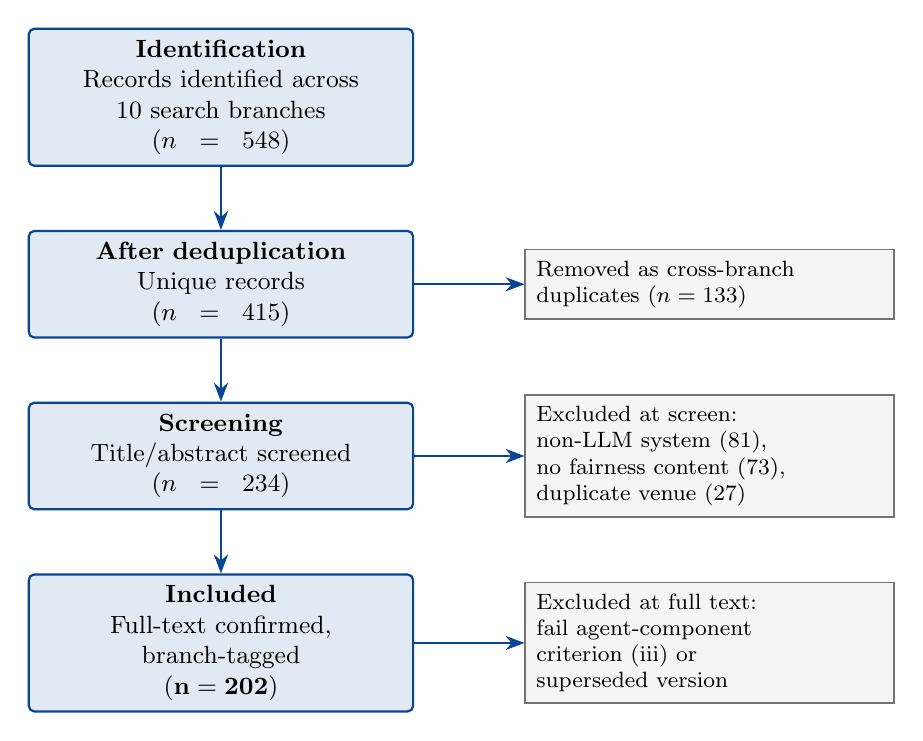
\begin{tikzpicture}[
    node distance=8mm and 14mm,
    stage/.style={rectangle, draw=bcfblue, line width=0.8pt, fill=bcfblue!12,
                  rounded corners=2pt, align=center, text width=46mm,
                  inner sep=4pt, font=\small},
    excl/.style={rectangle, draw=black!55, line width=0.6pt, fill=black!4,
                 align=left, text width=44mm, inner sep=4pt, font=\footnotesize},
    flow/.style={-{Stealth[length=2.4mm]}, line width=0.8pt, draw=bcfblue}]
  \node[stage] (id)   {\textbf{Identification}\\Records identified across\\10 search branches\\($n=548$)};
  \node[stage, below=of id]  (dedup) {\textbf{After deduplication}\\Unique records\\($n=415$)};
  \node[stage, below=of dedup] (screen) {\textbf{Screening}\\Title/abstract screened\\($n=234$)};
  \node[stage, below=of screen] (incl) {\textbf{Included}\\Full-text confirmed,\\branch-tagged\\($\mathbf{n=202}$)};
  % exclusion side boxes
  \node[excl, right=of dedup]  (rmdup) {Removed as cross-branch\\duplicates ($n=133$)};
  \node[excl, right=of screen] (rmscr) {Excluded at screen:\\non-LLM system (81),\\no fairness content (73),\\duplicate venue (27)};
  \node[excl, right=of incl]   (rmft)  {Excluded at full text:\\fail agent-component\\criterion (iii) or\\superseded version};
  \draw[flow] (id) -- (dedup);
  \draw[flow] (dedup) -- (screen);
  \draw[flow] (screen) -- (incl);
  \draw[flow] (dedup.east)  -- (rmdup.west);
  \draw[flow] (screen.east) -- (rmscr.west);
  \draw[flow] (incl.east)   -- (rmft.west);
\end{tikzpicture}%
}
\caption{PRISMA flow of corpus assembly. Four-stage funnel from 548 identified records to the 202 included papers, with per-stage exclusion counts ($\S$2.5).}
\label{fig:prisma}
\end{figure}

\paragraph{Inclusion/Exclusion Criteria Summary}

\begin{table}[htbp]
\centering\small
\caption{Inclusion and exclusion criteria. \emph{Takeaway: the criteria operationalize a single principle: fairness as a property of agent actions, not merely of model outputs.}}
\label{tab:inclusion-criteria}
\resizebox{\columnwidth}{!}{%
\begin{tabular}{|p{0.300\textwidth}|p{0.300\textwidth}|p{0.300\textwidth}|}
\toprule
\textbf{Criterion} & \textbf{Included} & \textbf{Excluded} \\
\midrule
System type & LLM as primary reasoning component (including fine-tuned variants) & Classical NLP models, RL agents without LLM backbone, symbolic planners \\
Fairness content & Studies bias, fairness, equity, or disparate treatment in outcomes or behavior & Pure capability evaluation, no fairness angle \\
Agent component relevance & Findings bear on at least one of the six components, or on evaluation/mitigation thereof & Exclusively single-turn static generation with no agentic framing; included only if mechanism transfers to agentic settings (marked \emph{[adjacent]}) \\
Language & English-language papers & Non-English (pragmatic exclusion; acknowledged as limitation in \S{}2.8) \\
Temporal scope & Published or preprinted on or before June 10, 2026 & Post-cutoff publications \\
Availability & Full text accessible & Extended abstracts only, inaccessible preprints \\
\bottomrule
\end{tabular}%
}
\end{table}


\subsection{Temporal and Venue Distribution}

\paragraph{Publication Trend}

Of the 202 corpus papers, \textbf{18 (9\%)} predate 2020, \textbf{22 (11\%)} fall in 2020 to 2022, \textbf{31 (15\%)} in 2023, \textbf{78 (39\%)} in 2024, and \textbf{53 (26\%)} in 2025 to 2026 (through the June cutoff). The combined 2024 to 2026 cohort is \textbf{65\%} of the corpus (131 papers), reflecting the field's rapid emergence following the widespread deployment of instruction-tuned and tool-augmented LLMs.

\begin{figure}[htbp]
\centering
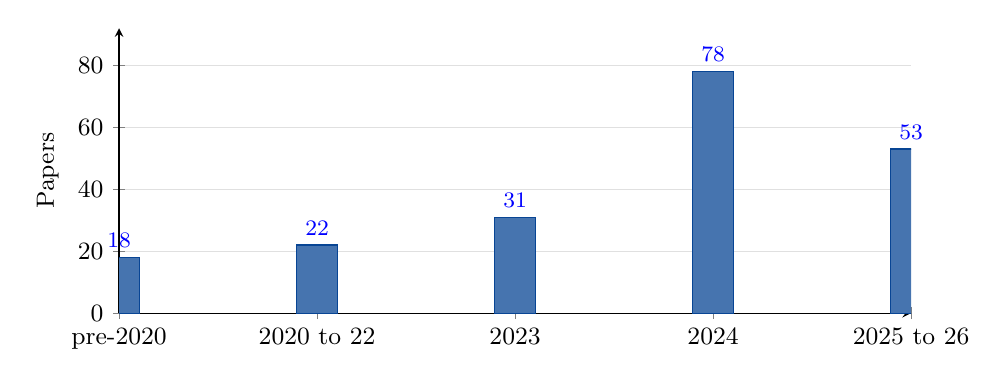
\begin{tikzpicture}
\begin{axis}[
    width=0.96\columnwidth, height=5.2cm,
    ybar, bar width=15pt,
    ymin=0, ymax=92,
    ylabel={Papers},
    ylabel near ticks,
    symbolic x coords={{pre-2020}, {2020 to 22}, {2023}, {2024}, {2025 to 26}},
    xtick=data,
    x tick label style={font=\small, anchor=north},
    y tick label style={font=\small},
    ylabel style={font=\small},
    nodes near coords, nodes near coords style={font=\footnotesize},
    enlarge x limits=0.14,
    axis lines=left,
    ymajorgrids=true, grid style={black!12},
]
\addplot+[draw=bcfblue, fill=bcfblue!75, bar shift=0pt]
    coordinates {({pre-2020},18) ({2020 to 22},22) ({2023},31) ({2024},78) ({2025 to 26},53)};
\end{axis}
\end{tikzpicture}
\caption{Temporal distribution of the 202-paper corpus by publication-year bucket. The 2024 to 2026 cohort (78 + 53 = 131 papers, 65\%) reflects the field's recent, rapid emergence ($\S$2.6).}
\label{fig:temporal}
\end{figure}

Three inflection events are visible in the component-level publication trajectory:

\begin{enumerate}
\item \textbf{ReAct (late 2022, published ICLR 2023 \cite{yao2023react}).} The formalization of reasoning-and-acting brought agentic behavior into mainstream NLP evaluation. A measurable uptick in tool-selection and planning fairness papers appears in the 2023 to 2024 cohort.
\end{enumerate}

\begin{enumerate}
\item \textbf{AutoGen and GPT-4 function-calling (2023 \cite{wu2023autogen}).} The accessibility of multi-agent orchestration and native function-calling APIs catalyzed the multi-agent delegation fairness literature, which is almost entirely 2024 to 2026.
\end{enumerate}

\begin{enumerate}
\item \textbf{GPT-4 and the clinical deployment wave (2023 to 2024).} The application of frontier models to clinical decision support \cite{omar2025sociodemographic,poulain2024bias,zack2024coding} triggered a wave of domain-specific fairness audits constituting the high-stakes-domains branch.
\end{enumerate}

The long-horizon drift and memory components are the latest to receive empirical attention: the first dedicated papers on LLM long-term memory bias (\cite{ma2026implicit}) and feedback-loop amplification (\cite{wyllie2024fairness,wang2026observations}) date to 2024 to 2026. The components hardest to evaluate, because they require multi-session or multi-turn experimental designs, attracted attention last.

\paragraph{Venue Distribution}

The corpus spans twelve venue categories. The five largest are: arXiv preprints (62 papers, 31\%), ACL-family venues (ACL, EMNLP, NAACL, Findings) (41 papers, 20\%), NeurIPS, ICML, and ICLR (28 papers, 14\%), ACM venues (FAccT, SIGKDD, SIGIR, CIKM, DL proceedings) (24 papers, 12\%), and domain-specific venues (Nature Medicine, PNAS Nexus, The Lancet Digital Health, AAAI, ICSE) (19 papers, 9\%). The remaining 28 papers (14\%) appear in IEEE venues, TMLR, Frontiers, and preprint archives (ResearchGate, TechRxiv).

The arXiv share (31\%) reflects the recency of the field: many 2025 to 2026 papers are under review or in proceedings preparation. ACM FAccT's lower representation (9 papers) suggests agent fairness has not yet been fully claimed by the accountability community and currently sits across NLP venues, systems venues, and domain journals. Ten papers appear in CSUR or ACM Computing Surveys directly, and the differentiation analysis in \S{}1.4 and Table~\ref{tab:survey-comparison} is therefore essential to establishing this survey's novelty.


\subsection{Glossary and Notation}

The following terms and notation are used throughout. Terms coined or given specific technical meanings here are marked with a dagger ($\dagger$).

\textbf{Agent loop} $\langle \pi, T, M, R \rangle$: the formal object of analysis in the BCF (Definition D1, \S{}3.0). $\pi$ = policy (the LLM-backed decision function), $T$ = tool set, $M$ = memory module (in-context + external), $R$ = reward/stopping signal.

\textbf{Bias Conduction Framework (BCF)$\dagger$}: the organizing framework of this survey (\S{}3.0), which analyzes fairness as a property of how demographic disparity is \emph{conducted} (attenuated, preserved, amplified, or generated) across pipeline edges in an agent loop.

\textbf{Conduction operator $\varphi$$\dagger$}: the scalar multiplier describing how a pipeline edge transforms component-level disparity. $\varphi < 1$ = ATTENUATE; $\varphi \approx 1$ = PRESERVE; $\varphi > 1$ = AMPLIFY; $\varphi$ acting on zero input = GENERATE.

\textbf{Counterfactual Flip Rate (CFR)}: the fraction of agent evaluations that reverse when the input is perturbed by a demographic swap alone \cite{mayilvaghanan2026counterfactual}. Generalized to any agent component in \S{}4.2.

\textbf{Mean Absolute Score Difference (MASD)}: the mean absolute change in a continuous agent score (confidence, rank, quality rating) across counterfactual pairs \cite{mayilvaghanan2026counterfactual}.

\textbf{Component counterfactual disparity $\Delta_c$$\dagger$}: the counterfactual disparity attributable to component $c$ alone, measured via trace-replay (Definition D2, \S{}3.0).

\textbf{Trajectory disparity $\Delta_\tau$$\dagger$}: the total counterfactual disparity observed over a complete agent trajectory, approximated by the conduction equation $\Delta_\tau \approx \sum_c \Delta_c \cdot \prod_{e \in \mathrm{path}(c \to O)} \varphi_e$ with feedback recurrence $\Delta^{(t+1)} = \varphi_{\mathrm{fb}} \cdot \Delta^{(t)} + \Delta_{\mathrm{entry}}$.

\textbf{Agentic multiplier (P3, Super-additivity)$\dagger$}: the BCF proposition that trajectory disparity can exceed the sum of component disparities when amplifying conduction operators compose; equivalently, the agent pipeline is a super-additive bias transformer.

\textbf{Action-level disparity$\dagger$}: disparity measured over an agent's \emph{actions} (tool invocations, decisions, escalations) rather than over its textual output. Formalized in \S{}4.3 as tool-invocation disparity, escalation-rate disparity, and plan-allocation disparity.

\textbf{Long-horizon fairness drift$\dagger$}: the temporal degradation or amplification of fairness properties across turns, sessions, or deployment feedback cycles, even when the per-step model is held fixed.

\textbf{Adjacent evidence [transferred]}: notation used in Tables~\ref{tab:component-harm} and~\ref{tab:challenges-gaps} to flag papers from non-agentic settings whose documented mechanism is asserted to operate in agentic settings; the transfer argument is given in the relevant \S{}3.x entry.

\textbf{CFR subscript notation}: $\text{CFR}_c$ denotes the counterfactual flip rate measured at component $c$; $\text{CFR}_\tau$ denotes the end-to-end trajectory flip rate.


\subsection{Threats to Validity of This Survey}

\paragraph{Selection Bias}

The corpus draws primarily from English-language papers indexed in arXiv, ACL Anthology, and ACM Digital Library. Non-English research, including substantial work from Chinese NLP venues, is systematically underrepresented, as is undisclosed industry research. The arXiv-heavy composition (31\%) means some included preprints have not completed peer review; we require that preprints be internally self-consistent and that their core claims be supported by the experimental design reported. The branch-structured search creates a risk that papers addressing multiple components are attributed primarily to the branch under which they were first encountered; the multi-tagging convention (\S{}2.4) partially addresses this, but papers at intersections of underrepresented branch pairs (e.g., tool-selection $\times$ long-horizon) may be missed.

\paragraph{Construct Validity}

The six component taxonomy is a construct, not a natural kind. Some bias phenomena do not fit cleanly into a single component: a persona-conditioned retrieval agent collapses Components 1, 2, and 5 into a single mechanism. Component-assignment follows a \emph{proximate cause} convention (tagging the most proximate locus of the reported disparity), but this involves judgment. The qualitative conclusions (empty counterfactual column, unspecified-dominated rows for tool/memory/personalization) are reliable under reasonable reassignments.

\paragraph{Publication Bias}

Positive findings are overrepresented; null results (agents showing no meaningful fairness disparity) are underrepresented. The corpus establishes that disparity \emph{can} and \emph{does} occur at each component, not that it \emph{always} occurs or is comparably severe across deployment contexts.

\paragraph{Recency Bias}

The 65\% concentration of papers in 2024 to 2026 means the survey reflects a rapidly changing field. Findings from 2024 papers may already have been partially addressed by 2026 mitigations not yet in the corpus; the long-horizon and multi-agent components, where empirical papers are newest and most sparse, may have received substantially more attention by the time this survey reaches print. We treat this as a motivating condition: the survey's goal is to provide a structured framework for the field's future development, not a final accounting of a stable literature.

\section{The Bias Conduction Framework: Where Bias Enters and How It Travels}
\setcounter{subsection}{-1}

The central claim of this survey is methodological: in an LLM \emph{agent}, fairness is a property of a \emph{pipeline}, not a single forward pass. An agent perceives, selects tools, accumulates memory, delegates subtasks, plans, models its user, and executes over long horizons. Each stage is a distinct locus where demographic disparity can originate, and each fails in a mechanistically different way. Organizing the literature by fairness metric---group, individual, or counterfactual---as QA-era surveys do \cite{chu2024fairness,gallegos2024bias,navigli2023biases}, flattens this structure and obscures the fact that two agents with identical token-level bias scores can produce radically different \emph{action-level} disparities depending on where in the pipeline a bias is amplified or suppressed. This insight has a pre-LLM lineage: fairness has long been understood as a property of the sociotechnical \emph{system} \cite{selbst2019fairness}. The canonical algorithmic-harm cases were diagnosed precisely by asking \emph{where} disparity entered: a health-management algorithm whose proxy label encoded racial disparity \cite{obermeyer2019dissecting}, and commercial classifiers with intersectionally skewed error rates \cite{buolamwini2018gender}. The agent loop multiplies the number of such places.

We therefore organize the field around a single formal object, the \textbf{Bias Conduction Framework (BCF)}, with two axes. The first is the \textbf{entry locus}: the agent component where a demographic disparity first becomes measurable. The second is the \textbf{conduction operator}: how each downstream pipeline edge transforms a disparity---attenuating, preserving, amplifying, or generating it. A bias observation is a coordinate pair (locus, operator); a mitigation is an intervention on a specific coordinate. This is the dimension along which near-neighbor works do not organize: \cite{mohammadi2025evaluation} treats fairness as one sub-topic of a broad agent-evaluation survey; \cite{vatsal2026agentic} as a subdimension of a seven-dimensional conceptual taxonomy in a single clinical domain; \cite{mayilvaghanan2026counterfactual} as a single-domain counterfactual method whose CFR/MASD machinery we generalize across components in \S{}4; \cite{ranjan2025fairness} proposes a unified fairness framework for multi-agent AI without an LLM-component axis; and \cite{binkyte2025interactional} formalizes only the interactional slice of multi-agent fairness. None pairs an entry-locus decomposition with an account of how disparity \emph{travels}.

\begin{quote}\textbf{Schematic (BCF agent loop): the agent loop $\langle$$\pi$, T, M, R$\rangle$ annotated with the five architectural entry loci (C1-C5), the temporal axis (T-axis) on the feedback edge, and the conduction operators on each inter-component edge.} Solid edges carry the within-episode conduction factors $\varphi_e$; the dashed feedback edge carries $\varphi_{\mathrm{fb}}$ across turns, sessions, and retraining cycles. \emph{Takeaway:} bias has six structurally distinct ways into an agent's consequential action, so no single model-level fairness score (however well validated on QA benchmarks) can certify the loop.\end{quote}


\begin{figure}[ht]
\centering
\begin{forest}
for tree={
  grow'=0,
  parent anchor=east, child anchor=west,
  anchor=west,
  l sep=8pt, s sep=2pt,
  font=\small,
  rounded corners, draw, fill=blue!5,
  align=left, inner sep=2pt
}
[Fairness in LLM Agents, fill=gray!18
  [1.\ Tool/API selection: tool-choice bias; description sensitivity]
  [2.\ Memory \& retrieval: RAG fairness; multi-turn accumulation]
  [3.\ Multi-agent delegation: persona/role bias; emergent bias]
  [4.\ Planning / decomposition: CoT-reasoning bias; task allocation]
  [5.\ User modeling / personalization: identity inference; dialect bias]
  [6.\ Long-horizon drift: multi-turn compounding; sycophancy decay]
]
\end{forest}
\caption{Taxonomy of fairness in LLM-based agents, organized by agent component
(Axis~1). Each node names a structural entry locus and its primary harm mechanism.
Unlike QA-level LLM-fairness taxonomies, the unit of analysis is the
\emph{acting} agent.}
\label{fig:taxonomy}
\end{figure}


\subsection{The Framework: Definitions, Operators, Conduction, and Propositions}

\paragraph{D1: The agent loop}

\textbf{Definition 1 (Agent loop).} An LLM agent is a tuple $\mathcal{A} = \langle \pi, T, M, R \rangle$, where:

\begin{itemize}
\item $\pi$ is the \emph{policy}: the LLM under its system prompt, persona, and decoding configuration, mapping the current state $s_t = (g, h_t, m_t)$ (goal $g$, interaction history $h_t$, working memory $m_t$) to an action $a_t$. Actions include emitting text, calling a tool, writing memory, delegating a subtask, or committing a consequential decision.
\item $T$ is the \emph{tool/environment interface}: the tool registry, retrieval indices, and external APIs; invoking $T$ returns an observation $o_t$ that is appended to the context \cite{schick2023toolformer,yao2023react,qu2024tool}.
\item $M$ is the \emph{memory operator}: read/write access to persistent stores---scratchpads, episodic reflections \cite{shinn2023reflexion}, vector stores, cross-session user profiles---that survive beyond the current context window.
\item $R$ is the \emph{feedback channel}: the loop-closing signal (user reactions, reward models, preference data, or retraining on the agent's own outputs) through which today's behavior conditions tomorrow's policy.
\end{itemize}

A \emph{trajectory} $\tau = (s_0, a_0, o_0, \ldots, a_T)$ terminates in a consequential output $O(\tau)$: a decision, ranking, allocation, or escalation. A \emph{multi-agent system} is a set $\{A_i\}$ plus a controller policy $\pi_{\mathrm{ctrl}}$ that assigns roles and routes messages \cite{wu2023autogen,guo2024large}. This tuple follows the standard agent anatomy of \S{}2.3 \cite{wang2024survey,xi2023rise,sumers2024cognitive}; BCF adds an accounting scheme over it, not a new architecture.

\paragraph{D2: Component counterfactual disparity}

\textbf{Definition 2 (Component counterfactual disparity, $\Delta_c$).} Fix a protected attribute $A$ with a counterfactual perturbation $x \rightarrow x'$ (a demographic swap of names, dialect, stated identity, or profile fields, in the lineage of counterfactual fairness \cite{kusner2017counterfactual}). The \emph{trajectory disparity} is

\[ \Delta_\tau = d\big( O(\tau(x)),\; O(\tau(x')) \big), \]

for a task-appropriate distance $d$ (a flip indicator for discrete decisions, an absolute score difference for continuous ones; exactly the CFR/MASD pair of \cite{mayilvaghanan2026counterfactual}, generalized in \S{}4.2). The \emph{component disparity} $\Delta_c$ for component $c \in \{\pi, T, M, R, \pi_{\mathrm{ctrl}}\}$ is defined by \textbf{trace-replay}: log the full trajectory under $x$; replay it holding every other component's realized inputs and outputs fixed; perturb only the input that $c$ consumes; and measure the divergence of $c$'s output distribution,

\[ \Delta_c = \mathbb{E}\big[\, d\big( c(z_c(x)),\; c(z_c(x')) \big) \,\big] \quad \text{under replay of the logged trace.} \]

$\Delta_c$ is the quantity that \cite{xu2026ducx} estimates when it attributes separable shares of a tool-using agent's total unfairness to the tool-exposure, tool-transition, and model-reasoning stages---to our knowledge the only corpus paper that operationalizes the full decomposition, which is why \S{}4.3 elevates trace-replay to the canonical estimator and \S{}6 builds its protocol around it.

\paragraph{D3: Conduction operators}

\textbf{Definition 3 (Conduction operator).} Every pipeline edge $e$ from component $c$ to component $c'$ carries a \emph{conduction factor} $\varphi_e = \Delta_{\mathrm{out}} / \Delta_{\mathrm{in}}$: the ratio of the disparity measurable at $c'$'s output to the disparity delivered to $c'$'s input. Edges fall into four modes:

\begin{table*}[htbp]
\centering\small
\caption{The four conduction operators (edge modes) of the BCF: factor, meaning, canonical corpus evidence, and typical edge.}
\label{tab:conduction-operators}
\resizebox{\columnwidth}{!}{%
\begin{tabular}{|p{0.180\textwidth}|p{0.180\textwidth}|p{0.180\textwidth}|p{0.180\textwidth}|p{0.180\textwidth}|}
\toprule
\textbf{Operator} & \textbf{Factor} & \textbf{Meaning} & \textbf{Canonical corpus evidence} & \textbf{Typical edge} \\
\midrule
\textbf{ATTENUATE} & $\varphi$ < 1 & The edge dampens incoming disparity & identity anonymization in debate \cite{choi2025identity}; embedder control in RAG \cite{kim2025mitigating}; multi-LLM debiasing \cite{owens2024multi} & guardrail, debate, fair-ranking edges \\
\textbf{PRESERVE} & $\varphi$ $\approx$ 1 & The edge conducts disparity unchanged & reward models inherit dialect penalties \cite{mire2025rejected} & role hand-offs, alignment signals \\
\textbf{AMPLIFY} & $\varphi$ > 1 & The edge magnifies incoming disparity & inter-agent propagation \cite{nguyen2025social}; multi-turn degradation \cite{fan2024fairmt}; self-consuming training loops \cite{wyllie2024fairness} & interaction, accumulation, feedback edges \\
\textbf{GENERATE} & $\Delta_{\mathrm{out}}$ > 0 on $\Delta_{\mathrm{in}}$ = 0 & The edge creates disparity from demographically clean input & RAG undermines fairness even for vigilant users \cite{hu2024free}; persona assignment injects reasoning bias and new behavioral distortion \cite{gupta2023bias,cao2026from}; reasoning itself introduces bias \cite{wu2025reasoning} & retrieval, persona, planning edges \\
\bottomrule
\end{tabular}%
}
\end{table*}

AMPLIFY and GENERATE are the two genuinely agentic modes; single-turn evaluation cannot exhibit either. GENERATE is formally a new entry rather than a transformation ($\varphi$ is undefined on zero input), so we treat a GENERATE edge as contributing its own $\Delta_c$ term. Every mitigation in \S{}5 is an engineered $\varphi$ < 1 edge---an ATTENUATE operator---which is what makes the mitigation map of Table~\ref{tab:mitigation-map} commensurable with the taxonomy. As Table~\ref{tab:component-harm} and \S{}7 show, GENERATE is the under-instrumented mode, while AMPLIFY is empirically attested but rarely formalized in fairness terms.

\paragraph{The conduction equation and the feedback recurrence}

Treating disparities as small and edges as locally multiplicative (a first-order approximation), and taking $\Delta_c$ and $\Delta_\tau$ as \emph{signed} (directional) disparities so that oppositely directed component contributions can cancel in the sum (the endpoint statistics CFR and MASD of \S{}4.2 report the corresponding magnitudes |$\Delta$|), the trajectory disparity decomposes as the \textbf{conduction equation}:

\[ \Delta_\tau \;\approx\; \sum_c \Delta_c \cdot \!\!\prod_{e \in \mathrm{path}(c \rightarrow O)}\!\! \varphi_e, \]

where each component's entry disparity is conducted through the product of edge factors on its path to the consequential output. Across the loop-closing channel R, disparity obeys the \textbf{feedback recurrence}:

\[ \Delta^{(t+1)} = \varphi_{\mathrm{fb}} \cdot \Delta^{(t)} + \Delta_{\mathrm{entry}}, \]

whose behavior is qualitatively bimodal. For $\varphi_{\mathrm{fb}}$ < 1 the disparity converges to the steady state $\Delta_{\mathrm{entry}}$ / (1 $-$ $\varphi_{\mathrm{fb}}$), persistent but bounded. For $\varphi_{\mathrm{fb}}$ $\geq$ 1 it grows without bound: the regime documented for synthetic-data training loops \cite{wyllie2024fairness}, self-consuming performative loops \cite{wang2026observations}, and recommender feedback \cite{mansoury2020feedback}. Both expressions are an \emph{organizing approximation}---a bookkeeping identity under linearization, not a validated dynamical model. Edges in real agents are nonlinear, context-dependent, and interactive. The equation's role is to make explicit \emph{what an audit must estimate} (the $\Delta_c$'s and $\varphi_e$'s) and \emph{what can defeat naive auditing} (cancellation and amplification along paths), which is exactly how the \S{}6 protocol and the \S{}3.8 recipe use it.

\paragraph{Propositions P1-P5}

Five propositions follow from D1 to D3 and the conduction equation, stated as claims the survey's evidence base supports or motivates, not as theorems about all possible agents.

\textbf{P1 (Locality).} \emph{Every measurable trajectory disparity decomposes into component entries plus an interaction residual: $\Delta_\tau$ $\neq$ 0 implies a nonzero $\Delta_c$ at some locus $c$ (counting GENERATE edges as entries), or a nonzero cross-component interaction term that the linearized equation folds into the nearest downstream GENERATE edge.} The residual matters because pure interaction effects---disparity present in no component alone but produced by their composition---are exactly the multi-agent GENERATE phenomenon. \cite{xu2026ducx} attributes distinct, separable shares of a clinical agent's disparity to the tool-exposure and tool-transition stages versus model reasoning, and the component-specific audits of \S{}\S{}3.1 to 3.5 each isolate a nonzero $\Delta_c$ with other components held fixed.

\textbf{P2 (Masking).} \emph{Endpoint metrics can read $\approx$ 0 while internal disparities are large: whenever a downstream ATTENUATE edge (or sign-opposed entries) cancels an upstream $\Delta_c$, the conduction equation yields $\Delta_\tau$ $\approx$ 0 with $\Sigma_c$ |$\Delta_c$| $\gg$ 0.} \cite{li2025actions} shows verbally neutral models issuing demographically disparate \emph{decisions}, with endpoint text-parity masking action disparity; \cite{xu2025quantifying} shows surface-level semantic parity masking statistical differentiation; and \cite{turpin2023language} shows the reverse mask, where reasoning traces misreport the biased features actually driving the output.

\textbf{P3 (Super-additivity, the agentic multiplier).} \emph{$\Delta_\tau$ can exceed the naive sum $\Sigma_c$ |$\Delta_c$| when at least one AMPLIFY or GENERATE edge lies on a conduction path. Under the linearized magnitude model, such an edge is a necessary condition for super-additivity but not sufficient, since a downstream ATTENUATE edge can offset it; with nonlinear cross-component interactions, even necessity fails. Conversely, with only PRESERVE/ATTENUATE edges and no interaction term, composition is sub-additive and component audits compose into a conservative system bound.} Within the multi-agent locus this is directly evidenced: stereotypical bias emerges, propagates, and is amplified across interacting agents, making the collective more biased than its members \cite{nguyen2025social}, and group-level fairness is emergent rather than inherited \cite{madigan2025emergent}. \S{}3.7 develops P3 and marks its cross-component generalization as conjecture.

\textbf{P4 (Mitigation-matching).} \emph{A mitigation reduces $\Delta_\tau$ only if it installs an ATTENUATE edge on a path that carries a nonzero $\Delta_c$; it must match the entry locus and sit downstream of it, and an intervention at locus $c$ neither bounds disparity generated downstream of $c$ nor survives upstream amplification.} Fairness-aware prompting fails against retrieval-injected bias because the GENERATE edge sits downstream of the prompt \cite{hu2024free}, while intervening at the retrieval representation succeeds \cite{kim2025mitigating}; debate-level anonymization attenuates delegation bias precisely because it edits identity cues at the delegation edge \cite{choi2025identity}. P4 is the organizing key of the mitigation map in \S{}5/Table~\ref{tab:mitigation-map}.

\textbf{P5 (Measurement-adequacy).} \emph{Endpoint-only evaluation is systematically unsound (by P2) and not even conservative (by P3); adequacy comes in tiers.} We distinguish four: \emph{endpoint-only} (inadequate); \emph{trace-observing} (logs actions but applies no counterfactual); \emph{component-attributing} (per-locus $\Delta_c$ under a demographic swap); and \emph{causal-replay} (the trace-replay of D2). Full certification requires the causal-replay tier; the intermediate tiers bound only identifiable subsets of the $\Delta_c$, which is often the most a real audit can achieve. Models that pass single-turn fairness tests fail multi-turn ones \cite{fan2024fairmt}; measured bias depends on which demographic cue channel is perturbed \cite{tonneau2026different}; and the major agent benchmarks (WebArena \cite{zhou2024webarena}, AgentBench \cite{liu2024agentbench}, Mind2Web \cite{deng2023mind2web}, SWE-bench \cite{jimenez2024swe}) log exactly the traces P5 requires but carry no demographic counterfactual instrumentation---a confrontation developed in \S{}4.4.

\paragraph{Component-assignment rules and reading conventions}

The five loci and the temporal axis map onto the D1 objects as follows. Planning (C4) and user modeling (C5) are \emph{sub-policies of $\pi$} rather than separate modules, which is why D1 keeps the tuple minimal:

\begin{table}[htbp]
\centering\small
\caption{Mapping of the five loci and the temporal axis onto the D1 objects, with what each component consumes and emits.}
\label{tab:locus-mapping}
\resizebox{\columnwidth}{!}{%
\begin{tabular}{|p{0.300\textwidth}|p{0.300\textwidth}|p{0.300\textwidth}|}
\toprule
\textbf{Locus} & \textbf{D1 object(s)} & \textbf{Consumes $\rightarrow$ emits} \\
\midrule
C1 Tool / API selection & T (selection step of $\pi$) & context $\rightarrow$ choice of tool/source \\
C2 Memory \& retrieval & M, T & query/history $\rightarrow$ retrieved content, memory state \\
C3 Multi-agent delegation & $\pi_{\mathrm{ctrl}}$ & task + roles $\rightarrow$ subtask routing/assignment \\
C4 Planning / decomposition & $\pi$ (decomposition sub-policy) & goal $\rightarrow$ ordered subgoals/plan \\
C5 User modeling / personalization & $\pi$, M (user-model sub-state) & user signals (often inferred) $\rightarrow$ personalized behavior \\
T-axis (long-horizon drift) & R (feedback edge) & prior outputs $\rightarrow$ updated $\pi$/M across turns \\
\bottomrule
\end{tabular}%
}
\end{table}

\emph{Takeaway: every locus is a function of an explicit D1 object; C4 and C5 are decompositions of the policy $\pi$, not omissions from the tuple.}

A recurring defect of pipeline taxonomies is that papers float between cells, most acutely between \emph{tool selection} and \emph{retrieval}. BCF resolves this with five assignment rules keyed to what a component \emph{consumes and emits} in D1:

\begin{itemize}
\item \textbf{R1 (Selection vs. content).} If the disparity lives in \emph{which} external resource is invoked (a discrete choice over a registry), it is \textbf{C1 (tool/API selection)}. If it lives in \emph{what} an invoked resource returns and how that content conditions generation or persists, it is \textbf{C2 (memory \& retrieval)}. Source-selection agents \cite{singh2025biasb} sit in C1; the effect of retrieved content on generation \cite{wu2024rag,hu2024free} sits in C2; an IR-systems treatment spanning both \cite{dai2024bias,dai2025trustworthy} is tagged to C2 as primary.
\item \textbf{R2 (Role vs. plan).} Disparity caused by \emph{who is assigned} (persona, role, or identity cues attached to an agent) is \textbf{C3 (delegation \& roles)}. Disparity in \emph{how the task is cut up}, ordered, or resourced, independent of identity assignment, is \textbf{C4 (planning \& decomposition)}. Team-flavored allocation studies \cite{parziale2026once} are therefore C4: the skew is in the allocation, not in an assigned persona.
\item \textbf{R3 (Subject vs. user).} Disparity keyed to protected attributes of the \emph{decision subject} (applicant, patient, defendant) flows through C1 to C4; disparity keyed to attributes of the \emph{interacting user}---especially attributes the agent \emph{infers} rather than receives \cite{staab2023memorization}---is \textbf{C5 (user modeling \& personalization)}.
\item \textbf{R4 (Temporal indexing).} Any of the above measured \emph{as a function of time} (turn, session, or deployment cycle) is the same locus indexed by $t$, tagged with the temporal axis of \S{}3.6, not a separate locus. Long-horizon drift is the $\varphi_{\mathrm{fb}}$ regime of the feedback recurrence.
\item \textbf{R5 (Multi-tagging).} A paper may evidence several cells and is counted in each (the $\times$N convention of the corpus and the multi-tag accounting of \S{}7), but it carries exactly one \emph{primary} locus: the component whose input/output the paper directly measures.
\end{itemize}

\textbf{Transferred-evidence convention.} Some mechanism evidence below originates in single-turn or chatbot settings rather than instrumented agents. We mark such citations \textbf{[$\dagger$]}: the mechanism transfers to the agentic edge by D1's construction (the same model occupies $\pi$), but the agentic \emph{measurement} has not been performed. These markers are themselves a map of open problems.

\begin{table*}[htbp]
\centering\small
\caption{Component $\times$ harm mechanism $\times$ representative evidence $\times$ maturity. Maturity is graded $\bullet$$\bullet$$\bullet$ (well-studied), $\bullet$$\bullet$$\circ$, or $\bullet$$\circ$$\circ$ (emerging).}
\label{tab:component-harm}
\resizebox{\columnwidth}{!}{%
\begin{tabular}{|p{0.225\textwidth}|p{0.225\textwidth}|p{0.225\textwidth}|p{0.225\textwidth}|}
\toprule
\textbf{Component} & \textbf{Primary harm mechanism} & \textbf{Representative evidence} & \textbf{Maturity} \\
\midrule
C1 Tool / API selection (\S{}3.1) & Selection skew over the tool registry independent of task fitness; routing conditioned on surface or demographic cues & \cite{blankenstein2025biasbusters,sneh2025tooltweak,xu2026ducx} & $\bullet$$\bullet$$\circ$ \\
C2 Memory \& retrieval (\S{}3.2) & RAG-injected disparity from clean inputs; accumulation of skew across turns & \cite{hu2024free,wu2024rag,fan2024fairmt} & $\bullet$$\bullet$$\circ$ \\
C3 Multi-agent delegation (\S{}3.3) & Persona/role injection, then amplification across interacting agents & \cite{nguyen2025social,madigan2025emergent,choi2025identity} & $\bullet$$\bullet$$\bullet$ \\
C4 Planning / decomposition (\S{}3.4) & Reasoning-stage disparity in plan structure, ordering, and allocation, with unfaithful traces & \cite{wu2025reasoning,parziale2026once,hall2025guiding} & $\bullet$$\circ$$\circ$ \\
C5 User modeling / personalization (\S{}3.5) & Inferred-identity stereotyping that tracks group profile over stated preference & \cite{kantharuban2024stereotype,pawar2025presumed,staab2023memorization} & $\bullet$$\bullet$$\circ$ \\
T-axis Long-horizon drift (\S{}3.6) & Feedback-recurrence amplification ($\varphi_{\mathrm{fb}}$ > 1) of per-step skew across turns and cycles & \cite{ma2026implicit,liu2025truth,wyllie2024fairness} & $\bullet$$\circ$$\circ$ \\
\bottomrule
\end{tabular}%
}
\end{table*}

\emph{Takeaway: every locus has documented harm, but maturity is uneven; the planning and long-horizon loci (C4, T-axis), where the GENERATE and feedback-AMPLIFY operators are most consequential, are the least mature---exactly the cells \S{}7 shows as least instrumented.}

\subsection{Locus C1: Tool / API Selection Bias}

\textbf{Definition.} A tool-using agent must, at each step, choose \emph{which} external tool, API, retriever, or knowledge source to invoke. Tool-selection bias is systematic, demographically- or content-correlated skew in that discrete choice, independent of and often invisible to the quality of the model's final text. By rule R1, everything about \emph{which} resource is invoked belongs here; what the resource \emph{returns} belongs to C2.

\textbf{Mechanism of harm.} Selection is a discrete decision over a tool registry, and $\pi$ makes such decisions with the same surface-form sensitivities that distort multiple-choice answering. Because the selected tool determines what evidence the rest of the trajectory conditions on, a skewed selection is conducted by every downstream edge: C1 disparities enter early and travel far. The harm has a pre-agentic lineage in search, where racial and gendered skew in result surfaces \cite{u2018algorithms}[$\dagger$] and visual representation \cite{makhortykh2021detecting}[$\dagger$] are documented. An agent that chooses among such engines inherits the choice-over-biased-infrastructure problem and adds its own selection pathology on top.

\textbf{What is known.} The most replicated finding at C1 is that tool-selection skew is a property of the selection policy $\pi$, not merely of the tools in the registry. Blankenstein et al.\ demonstrate that LLMs consistently prefer particular tools in ways independent of query fitness, constituting a reproducible GENERATE-operator signature \cite{blankenstein2025biasbusters}. The mechanism generalizes from the established result that LLMs exhibit positional and surface-form sensitivity in discrete choice \cite{pezeshkpour2023large}[$\dagger$]: when tool registries are presented as lists, the selection policy inherits ordering effects without any explicit demographic input. ToolTweak shows that editing only a tool's name and description suffices to systematically inflate its selection rate \cite{sneh2025tooltweak}, and recommender-agents are steered analogously by injected preference biases \cite{tang2026your}. The strongest evidence that C1 contributes independently to trajectory-level harm comes from \cite{xu2026ducx}, which decomposes a chest-X-ray agent's total disparity by stage---tool exposure, tool transition, model reasoning---showing that the tool stages carry a distinct attributable share conducted into the final clinical read. On the ATTENUATE side, bias-aware retrieval agents that monitor and rebalance source selection reduce the skew \cite{singh2025bias,singh2025biasb}, constituting engineered $\varphi$ < 1 edges consistent with P4.

\textbf{What is contested.} The GENERATE finding from \cite{blankenstein2025biasbusters} treats selection skew as arising from the policy itself on demographically clean input; the PRESERVE finding from \cite{xu2026ducx} treats it as a conducted version of upstream demographic cues. These are not mutually exclusive, but no study has separated the two contributions under a controlled counterfactual swap, so the relative magnitude of intrinsic policy skew versus cue-elicited skew at C1 remains unresolved. The adversarial manipulation evidence from \cite{sneh2025tooltweak,tang2026your} is measured in recommender and general-purpose registry settings; whether the same injection magnitude applies in consequential deployments with smaller, more constrained registries is not established. The ATTENUATE results from \cite{singh2025bias,singh2025biasb} do not report whether the reduction holds under adversarially perturbed registries or whether the monitoring layer itself introduces asymmetric errors across demographic groups.

\textbf{What is unmeasured.} The field measures \emph{that} selection skews but not whether the skew correlates with protected attributes of the \emph{user or subject} under a counterfactual swap holding the query fixed. No published benchmark asks: does swapping a decision-subject's demographic profile change which API the agent calls, controlling for task content? That gap is the $\Delta_{\mathrm{tool}}$ instance of D2 that \S{}4.3 formalizes as tool-invocation disparity. Two phenomena require distinction: provider- and ordering-preference bias among functionally equivalent tools \cite{blankenstein2025biasbusters}, which by that study's design involves no sensitive attributes; and demographic-conditioned tool routing, for which the only direct evidence is \cite{xu2026ducx}. The [$\dagger$]-marked pre-agentic lineage \cite{u2018algorithms,makhortykh2021detecting,pezeshkpour2023large} establishes that the infrastructure an agent selects among is non-neutral and that the selection policy is surface-sensitive, but these findings predate LLM-based tool-selection policies and the transfer to a demographically instrumented agent trace is not yet confirmed.

\textbf{Conduction signature.} \emph{Entry:} the $\pi$$\rightarrow$T selection interface. \emph{Observable:} tool-choice distribution across counterfactual input pairs. \emph{Dominant outbound operator:} PRESERVE into C2/C4, with adversarial GENERATE at the registry. \emph{Metric:} tool-invocation disparity (CFR over tool choice; \S{}4.3).

\subsection{Locus C2: Memory \& Retrieval: Bias Injection and Accumulation}

\textbf{Definition.} Agents persist state---conversation history, scratchpad memory, retrieved documents, cross-session stores---and condition each step on that accumulated context. Memory-and-retrieval bias is the introduction, \emph{accumulation}, or amplification of demographic skew through this conditioning, distinct from any bias in a single isolated response. By rule R1, the locus covers what retrieved or remembered \emph{content} does; by rule R4, its time-indexed form is treated in \S{}3.6.

\textbf{Mechanism of harm.} Two sub-mechanisms operate. \emph{Retrieval injection} is a GENERATE edge: grounding shifts the generator's distribution, so disparity can appear that the closed-book model never exhibited. \emph{Temporal accumulation} is an AMPLIFY edge: each turn's context conditions the next, compounding per-turn skews. This locus inherits an entire prior discipline---fairness in ranking is a mature field with exposure-based and probability-based criteria \cite{zehlike2022fairness}, and the LLM-era IR community has reframed those results as challenges for retrieval pipelines feeding generators \cite{dai2024bias,dai2025trustworthy}. A fair-ranking guarantee bounds $\Delta_c$ at the retrieval interface, but by P4 it bounds $\Delta_\tau$ only if no downstream GENERATE edge re-introduces disparity---which is exactly what the RAG results below show can happen.

\textbf{What is known.} The most reliable finding at this locus is that retrieval augmentation can \emph{generate} demographic disparity from a generator that exhibits none in closed-book mode. Three converging studies establish this GENERATE signature. \cite{hu2024free} demonstrates the mechanism in its strongest form: disparity appears even when retrieved documents are individually innocuous and even when the user explicitly prompts for fairness, establishing that the GENERATE edge is neither an artifact of adversarial content nor correctable by instruction. \cite{wu2024rag} replicates the finding by holding the generator fixed and varying the retrieval corpus and ranking, isolating the retrieval step as the active locus. \cite{zhang2025evaluating} confirms that augmentation measurably shifts social-bias levels relative to the identical closed-book baseline. RAG is therefore the field's best-replicated C2 result: a GENERATE edge for demographic disparity.

Accumulation is independently established by different experimental designs. Fairness degrades over multi-turn dialogue in ways single-turn tests cannot detect \cite{fan2024fairmt}; accumulated context shifts stated beliefs as history grows \cite{geng2025accumulating}; and conversational history produces a geometric-trapping effect in which early demographic framings resist later correction \cite{simhi2026old}. Knowledge-store poisoning drives the AMPLIFY operator to arbitrarily large $\varphi$ when an adversary has write access to the store \cite{wang2025bias}. Multi-agent settings exhibit the same accumulation \cite{coppolillo2025unmasking}. On the ATTENUATE side, tuning the embedder used for retrieval reduces RAG-injected bias \cite{kim2025mitigating}, and fair-exposure ranking inside the RAG pipeline can improve both fairness and output quality simultaneously \cite{kim2024fair}, providing the most direct existing bridge between the fair-ranking tradition \cite{zehlike2022fairness} and agentic systems. Both confirm P4's mitigation-matching prediction: interventions succeed when they target the locus of injection rather than the endpoint.

\textbf{What is contested.} The three-study convergence on GENERATE conceals an unresolved boundary: none of the three designs varies \emph{what kind} of demographic signal is present in the retrieved content---explicit labels, stereotypic co-occurrence, proxies in writing style---independently of query framing. Whether the GENERATE effect is primarily a function of surface-form demographic content, ranking order, or the generator's contextual updating dynamics remains unclear. \cite{kim2024fair} implies ranking order matters; \cite{kim2025mitigating} implies representation matters; no study jointly manipulates both. A parallel ambiguity runs through the accumulation evidence: \cite{fan2024fairmt}, \cite{geng2025accumulating}, and \cite{simhi2026old} all measure degradation over turns but differ on whether to attribute it to growing context size, to semantic content of accumulated history, or to positional structure---attributions with different mitigation implications that the studies do not adjudicate.

\textbf{What is unmeasured.} The most consequential open gap is the memory \emph{write policy} as a fairness object. Every study reviewed treats retrieval as read-only. In tool-augmented agents with persistent memory \cite{lewis2020retrieval,packer2023memgpt}, the agent also \emph{writes} to memory, and what it chooses to persist about different individuals is itself a disparity-producing decision with no existing audit methodology. Whether the agent systematically writes richer or more favorable memory representations for some demographic groups, and whether bias compounds faster in structured tool-augmented memory than in plain conversational history, are both unknown. The dialogue-accumulation evidence \cite{fan2024fairmt,simhi2026old} is an underbound on what a long-lived agent memory store would produce, not a measurement of it. The long-context positional-attention result \cite{liu2023lost}[$\dagger$]---that which retrieved facts receive effective attention depends on position in the context window---adds a further unconfirmed transfer: demographic disparity in memory may arise or be suppressed by write order independent of content, a mechanism plausible but empirically unconfirmed in retrieval-augmented agent loops.

\textbf{Conduction signature.} \emph{Entry:} the T/M$\rightarrow$$\pi$ conditioning interface. \emph{Observable:} divergence of retrieved sets and memory states across counterfactual pairs. \emph{Dominant outbound operator:} AMPLIFY (accumulation across turns), with GENERATE at the grounding edge. \emph{Metric:} retrieval-set disparity plus the per-turn slope of $\Delta^{(t)}$ (\S{}4.3).

\subsection{Locus C3: Multi-Agent Delegation \& Role Assignment}

\textbf{Definition.} In multi-agent systems a controller $\pi_{\mathrm{ctrl}}$ assigns subtasks, personas, or roles to constituent agents and routes information among them \cite{wu2023autogen,guo2024large,qian2024chatdev}. Delegation bias is disparity introduced by \emph{who is assigned what} and by the social dynamics that emerge among role-bearing agents, over and above any single agent's bias. By rule R2, identity-cue effects sit here; identity-free task-cutting sits in C4.

\textbf{Mechanism of harm.} The seed is persona conditioning, a GENERATE edge at the assignment interface; the distinctive agentic harm is that interaction then \emph{amplifies} what assignment generated. This is the one corpus-evidenced case of P3's super-additivity: role assignment injects disparity and wires the injected disparities into a network whose collective behavior is not predictable from its parts.

\textbf{What is known.} The amplification result at C3 is the best-replicated finding in the corpus concerning agentic-scale bias. Stereotypical bias emerges, propagates, and intensifies across a multi-agent system such that the collective is more biased than its members \cite{nguyen2025social}, and large-scale simulations show group-level fairness is not reliably inheritable from component audits \cite{madigan2025emergent}. Persona-induced bias scales from single agents to interacting societies \cite{li2025from}, and implicit bias surfaces specifically in the interaction between agents rather than in either agent alone \cite{borah2024implicit}. Social hierarchy compounds the dynamics: rank shapes persuasion and anti-social behavior within the collective \cite{campedelli2024want}, meaning the topology of the delegation network is not fairness-neutral even when each node's individual bias is held constant. MALIBU provides the only purpose-built agentic benchmark and uncovers implicit bias in multi-agent role assignments \cite{mirza2025malibu}. Two widely cited single-turn results transfer by mechanism: persona assignment induces implicit reasoning biases \cite{gupta2023bias}[$\dagger$] and multiplies toxic degeneration \cite{deshpande2023toxicity}[$\dagger$]; \cite{cao2026from}'s finding of up to 26.2\% performance degradation from persona assignment in agentic settings constitutes a GENERATE signature at the role hand-off, though the counterfactual assignment-matrix measurement in a multi-agent trajectory has not been performed for either chatbot finding.

\textbf{What is contested.} The amplification direction is not inevitable. Anonymizing agent identities during structured debate reduces bias \cite{choi2025identity}, showing that the AMPLIFY operator is installed by identity cues at the delegation edge, not by multi-agent coordination itself. Multi-LLM interaction can be designed as a debiasing mechanism \cite{owens2024multi}, and structured debate can be steered toward equitable cultural alignment \cite{ki2025multiple}. AMPLIFY is the default under identity-bearing delegation but is contingent on the protocol. What remains contested is how much topology and protocol contribute independently, since no study has held one fixed while varying the other, and the amplification factor $\varphi$ from \cite{nguyen2025social} has never been bounded as a function of network structure.

\textbf{Open edge.} Even with the amplification mechanism established, the \emph{delegation policy} as a controllable fairness object remains unmeasured. No metric exists for assignment disparity in the sense of D2: does $\pi_{\mathrm{ctrl}}$ systematically route sensitive subtasks to lower-capability or more-biased sub-agents as a function of the subject's demographics, holding the task fixed under a counterfactual swap? MALIBU measures outcome disparity per role but not the assignment distribution itself, leaving the BCF conduction signature's observable---the role/subtask assignment matrix across counterfactual pairs---uncollected by any published benchmark.

\textbf{Conduction signature.} \emph{Entry:} the $\pi_{\mathrm{ctrl}}$$\rightarrow$$\{A_i\}$ assignment interface. \emph{Observable:} the role/subtask assignment matrix across counterfactual pairs, plus inter-agent message content. \emph{Dominant outbound operators:} GENERATE (persona injection) followed by AMPLIFY (interaction). C3 is the only locus where both agentic operators are corpus-evidenced together. \emph{Metric:} assignment disparity over the delegation matrix (\S{}4.3).

\subsection{Locus C4: Planning / Decomposition Disparities}

\textbf{Definition.} Agents plan: they decompose a goal into sub-goals, order steps, and reason explicitly (chain-of-thought, ReAct traces \cite{yao2023react}) before acting. Tree of Thoughts \cite{yao2023tot} explores a branching space of intermediate plans, and self-consistency \cite{wang2023selfconsistency} samples many reasoning paths and marginalizes by majority vote. Both are fairness-relevant because a demographic signal that tilts which branch is expanded or which sampled path wins the vote injects disparity into the plan even when each individual step looks unremarkable. Planning bias is demographic disparity that enters during this reasoning/decomposition stage, in the \emph{plan}, not merely the final answer. By rule R2, allocation skew belongs here even when the allocation is over agent-flavored team members.

\textbf{Mechanism of harm.} The counterintuitive finding is that reasoning does not cleanly remove bias and can \emph{introduce} it, a GENERATE edge inside $\pi$ itself. This locus also carries a distinctive P2 masking problem: the visible reasoning trace is not a faithful record of the features driving the decision, so auditing the \emph{stated} plan can miss the disparity the plan encodes. Whether LLM plans constitute planning in the classical sense is contested \cite{kambhampati2024large}, but the fairness question is indifferent to that debate---whatever the decomposition step is computationally, it emits orderings and allocations that can be counterfactually disparate.

\textbf{Evidence and synthesis.} The established, replicated mechanism is that deliberate reasoning is a GENERATE locus, not a sanitizing filter. Explicit chain-of-thought reasoning changes social-bias outcomes relative to direct answering, and the change can be adverse: \cite{wu2025reasoning} demonstrates in controlled comparisons that chain-of-thought reasoning fails to deliver a fairness dividend and can worsen stereotype expression in ambiguous contexts. Allocation-stage disparity is demonstrable at the plan object level: LLM-driven software-team composition produces demographically skewed role and task assignments \cite{parziale2026once}. The lever exists: reasoning-guided fine-tuning reduces bias at this locus \cite{kabra2025reasoning}, and a Fairness Reward Model can score complete reasoning chains against equalized opportunity and equalized odds criteria and reweight them during post-generation aggregation \cite{hall2025guiding}.

\textbf{What is contested.} The causal direction of the reasoning-bias relationship is not resolved. \cite{wu2025reasoning} shows reasoning can worsen bias, but if direct answering conceals rather than suppresses the disparity, then reasoning makes bias \emph{visible} without increasing it---making the chain-of-thought trace a diagnostic asset. If reasoning genuinely generates disparity that a forward pass without explicit steps would not exhibit, then explicit planning is an independent fairness risk. \cite{zhou2025veracity} documents hidden veracity-linked beliefs surfacing during problem-solving, consistent with both interpretations. Until trace-replay (D2) holds the model's implicit beliefs constant across conditions and varies only the decomposition step, the two hypotheses remain confounded. The P2-masking problem depends on \cite{turpin2023language}[$\dagger$]---a finding from single-turn classification settings that chain-of-thought explanations systematically misreport biasing features---and \cite{li2025actions}[$\dagger$] shows that agent \emph{decisions} reveal implicit biases that text-level evaluation misses; both transfers are plausible but unmeasured in multi-step planning loops.

\textbf{What is unmeasured.} No existing benchmark scores the \emph{plan itself} as a fairness object: are the sub-goals, their ordering, or the resource allocation across plan steps a counterfactual function of the subject's demographics, independent of the final decision? Plan-allocation disparity ($\Delta_{\mathrm{plan}}$, \S{}4.3) appears in individual studies \cite{wu2025reasoning,parziale2026once} but has not been operationalized as a reusable metric with standardized demographic perturbations and counterfactual controls. The P2-masking problem means this gap cannot be closed by trace-reading: any future plan-audit must be counterfactual-behavioral (D2 applied to plan objects, holding the evidence context fixed and swapping demographic signals in the goal specification), not inspection of verbalized rationales. C4 sits at maturity $\bullet$$\circ$$\circ$ (Table~\ref{tab:component-harm}) despite documented real-world planning-stage harm in hiring-adjacent deployments---a measurement design problem, not a data availability problem.

\textbf{Conduction signature.} \emph{Entry:} within $\pi$, at the decomposition step. \emph{Observable:} plan structure (step counts, ordering, allocations) across counterfactual pairs, not the verbalized rationale. \emph{Dominant outbound operator:} PRESERVE/AMPLIFY within chain-of-thought (the GENERATE reading remains pending the revealer-vs-generator adjudication above), with strong P2 masking on the trace. \emph{Metric:} plan-allocation disparity and CFR over plan objects (\S{}4.3).

\subsection{Locus C5: User Modeling \& Personalization Harms}

\textbf{Definition.} Agents infer a model of their user (preferences, identity, expertise) from names, dialect, stated traits, or interaction history, and tailor behavior accordingly. Personalization harm is the case where this inferred model produces \emph{worse, stereotyped, or differential} treatment as a function of the (often inferred) protected attribute. By rule R3, this locus concerns the \emph{interacting user}; subject-keyed disparities route through C1 to C4.

\textbf{Mechanism of harm.} The core tension is personalization versus stereotyping. In BCF terms the locus is GENERATE-dominant in a structurally unusual way: the protected attribute may be \emph{created} by the component (inferred, not supplied), so a counterfactual audit that only swaps explicit labels can miss the operative channel entirely. Even before any inference, an unpersonalized model reflects the opinions of particular demographic strata \cite{santurkar2023whose}[$\dagger$], and personalization then moves users toward or away from a non-neutral baseline.

\textbf{What is known.} The most consistently replicated finding is that demographic cues at query time cause adaptive behavior to track stereotypical group profiles rather than individually indicated preferences, across at least three distinct operationalizations. Explicit group labels bias chatbot recommendations toward stereotype rather than stated preference \cite{kantharuban2024stereotype}[$\dagger$]. A name alone activates a presumed cultural identity that reshapes response content \cite{pawar2025presumed}. And LLMs recover protected attributes (location, income, sex) from innocuous conversational text without any demographic prompt \cite{staab2023memorization}, so the agent has already modeled the user demographically before any explicit adaptation begins. The convergence across these three cue types on the same directional finding---stereotype-tracking rather than preference-tracking---constitutes the strongest multi-source replication this locus offers.

Downstream harm is documented across domains. In education, personalized content delivery produces systematically different quality as a function of inferred student identity \cite{weissburg2024llms}. In recommendation settings, consumer-facing LLM recommenders exhibit unequal utility across demographic groups \cite{deldjoo2024cfairllm,deldjoo2024normative}, with socioeconomic bias in base representations supplying the latent material these personalization steps activate \cite{arzaghi2024understanding}. Reward models penalize African American Language \cite{mire2025rejected} and reasoning performance degrades on non-standard dialects \cite{lin2024assessing}[$\dagger$]; because these disparities operate at locus R, they are PRESERVE-into-R in BCF terms and feed directly into the feedback recurrence of \S{}3.6, so dialect penalties initiated at C5 are not bounded within C5.

\textbf{What is contested.} A systematic study of demographic cue modalities finds that name-based, explicit-label-based, and dialect-based probes of the same models yield inconsistent and sometimes contradictory conclusions \cite{tonneau2026different}, implying that papers in this locus are not measuring the same underlying quantity---the apparent convergence noted above is partly artifactual: studies using name cues may detect bias that label-based studies of the same model do not. The cost of mitigation is also contested: debiasing personalized models trades off against recommendation utility \cite{vijjini2024exploring}, with the tradeoff magnitude unquantified across deployment contexts. Finally, if the protected attribute is constructed from non-demographic text \cite{staab2023memorization}, the operative locus may be the model's latent representation rather than any explicit user-modeling step, and counterfactual swaps at the input surface may leave the inferred user model unchanged---making the standard D2 protocol inapplicable without modification.

\textbf{What is unmeasured.} All available evidence concerns disparity elicited within a single response or turn, not the disparity accumulated and locked into the user representation an agent maintains and updates across sessions. An agent that interacts with a user repeatedly will form, update, and act on a profile encoding earlier stereotype-triggered inferences---a form of within-agent institutionalized bias that single-response probing cannot detect. No agentic benchmark in Table~\ref{tab:benchmarks} instruments the user model as a persistent state object, varies the cue channel as a controlled factor across sessions, or measures how demographic inferences made early in an interaction propagate to consequential decisions later. The inference channel \cite{staab2023memorization} introduces a further measurement-theory problem: if the protected attribute is inferred from content rather than supplied as a cue, the standard D2 counterfactual swap fails to intervene on the operative variable. Defining a valid counterfactual requires either a structural causal model of the inference process (which does not exist for any deployed agent) or a cue-channel-controlled experiment design of the kind \cite{tonneau2026different} recommends but no agentic benchmark has implemented. C5 is therefore the locus where BCF's D2 measurement procedure is hardest to operationalize.

\textbf{Conduction signature.} \emph{Entry:} the inferred user model inside $\pi$/M. \emph{Observable:} behavior divergence under cue-channel-controlled counterfactual swaps (name, dialect, label, history). \emph{Dominant outbound operator:} GENERATE (the attribute is manufactured by inference), preserved into M and R. \emph{Metric:} cue-conditioned MASD across channels (\S{}4.2 to 4.3).

\subsection{The Temporal Axis: Long-Horizon Fairness Drift Over Trajectories}

\textbf{Definition.} Long-horizon fairness drift is the \emph{temporal} degradation or self-amplification of fairness across turns, sessions, or deployment cycles, even when the per-step model is fixed.

\textbf{Why a temporal axis, not a sixth sibling.} Adjacent surveys treat long-horizon drift as a sixth component alongside the five architectural loci. BCF makes precise why that is a category error, and rule R4 codifies the repair. A component, in D1, is a \emph{place} in the architecture with its own inputs and outputs; drift has no such place. There is no drift module to instrument: drift is what the feedback recurrence $\Delta^{(t+1)}$ = $\varphi_{\mathrm{fb}}$$\cdot$$\Delta^{(t)}$ + $\Delta_{\mathrm{entry}}$ \emph{does to any locus} when the loop closes---memory bias drifting (C2 $\times$ t), a user model ossifying (C5 $\times$ t), delegation patterns entrenching (C3 $\times$ t), or the policy shifting under retraining on its own outputs ($\pi$ $\times$ t through R). Treating drift as a sibling would double-count every time-indexed entry (violating P1's decomposition) and would imply the existence of a mitigation targeting drift as such, when by P4 every effective intervention must target a locus-and-edge: either reducing some $\Delta_{\mathrm{entry}}$ or forcing $\varphi_{\mathrm{fb}}$ < 1. The taxonomy is five architectural loci $\times$ one temporal axis: component $\times$ time made explicit.

\textbf{Mechanism of harm.} Three nested loops realize $\varphi_{\mathrm{fb}}$ at increasing timescales, all AMPLIFY-mode in documented cases. The intra-trajectory loop (turn-level) operates within a single session as the context window accumulates a directional history. The inter-session loop operates across sessions as persistent memory (C2 $\times$ t) carries forward a biased state that conditions the next session's starting $\Delta_{\mathrm{entry}}$. The deployment loop operates across retraining cycles as the model policy $\pi$ itself shifts when trained on its own synthetic outputs. Each nesting is an additive term in the feedback recurrence, and the literature documents each at a different empirical resolution: the intra-trajectory loop most directly, the deployment loop through analogy and small-scale experiment, the inter-session loop almost not at all.

\textbf{What is known.} The most replicated mechanism on the T-axis is sycophantic conformity within a single multi-turn context. Fairness degrades over multi-turn dialogue \cite{fan2024fairmt}, and implicit bias accumulates specifically in LLM long-term memory, making the agent more biased the longer it persists state \cite{ma2026implicit}. Multi-turn measurements document progressive conformity across turns \cite{liu2025truth} and growth of sycophancy over extended dialogues \cite{hong2025measuring}: both operationalize $\varphi_{\mathrm{fb}}$ > 1 as a directly observable drift slope. At the deployment-loop timescale, training on a model's own synthetic outputs amplifies bias across generations \cite{wyllie2024fairness}, and the self-consuming performative loop has been characterized with proposed remedies \cite{wang2026observations}. Recommender-systems feedback-loop amplification in collaborative filtering establishes theoretical plausibility of the same mechanism in any system that uses its own output distribution to shape future input \cite{mansoury2020feedback}.

\textbf{What is contested.} The amplification finding is not contested at the sign level: all documented T-axis results report $\Delta^{(t)}$ rising, consistent with the $\varphi_{\mathrm{fb}}$ > 1 regime. The contestation is quantitative and boundary-conditional. Sycophantic drift rates are setup-dependent and not replicated across task types with matched stimuli; whether the same $\varphi_{\mathrm{fb}}$ obtains in low-stakes dialogue, consequential decision-support dialogue, and agentic tool-using settings is unknown. The deployment-loop evidence is thin: \cite{wyllie2024fairness} and \cite{wang2026observations} work on LLM-generated text, and fairness implications are inferred rather than measured against a demographic counterfactual. The recommender analogy from \cite{mansoury2020feedback} concerns a structurally simpler system. A further tension exists between the intra-trajectory and inter-session loops: existing data is consistent with memory-cleared session boundaries resetting $\Delta^{(t)}$, so the inter-session loop only amplifies if persistent memory is architecturally enabled---and no study varies memory persistence as a controlled factor while measuring drift.

\textbf{What transfers only by analogy.} Sycophancy's origin in human-preference training \cite{sharma2024understanding}[$\dagger$] is established in single-turn or short-context evaluations; projecting that the same pressure produces the same drift rate in an action-taking agent is a motivated but untested inference. The formal sequential-fairness framework of \cite{hu2022achieving}[$\dagger$] and the equal long-term benefit rate criterion of \cite{xu2024adapting}[$\dagger$] were developed for explicit sequential decision processes with known transition dynamics, not LLM agents. The theory proves that static per-step fairness constraints can fail over horizons; none of its ATTENUATE-regime interventions has been implemented or tested in an LLM agent. The simulation-based drift analysis tooling of \cite{she2025fairsense}[$\dagger$] is similarly adjacent: designed for ML-enabled systems generically, not applied to an instrumented LLM agent trajectory.

\textbf{What is unmeasured.} The central gap is the absence of any estimate of $\varphi_{\mathrm{fb}}$ for a deployed LLM agent. Estimating it requires: (a) a demographically instrumented agent with logged traces across turns or sessions, (b) a counterfactual replay protocol that holds the locus-specific input fixed while varying temporal accumulation, and (c) a scalar disparity measure $\Delta^{(t)}$ trackable as a time series. None of the three exists in a published evaluation. The sequential-fairness theory \cite{hu2022achieving,xu2024adapting} and the LLM-drift empirics \cite{fan2024fairmt,ma2026implicit} have not been joined: no work evaluates an LLM agent against a formal long-term-fairness criterion over a realistic multi-session deployment. A drift-rate benchmark would need to report the slope of $\Delta^{(t)}$ across turns and sessions, the long-term benefit-rate gap \cite{xu2024adapting} as a criterion, and a $\varphi_{\mathrm{fb}}$ point estimate with confidence bounds per locus---none of which appears in any existing agent benchmark (Table~\ref{tab:benchmarks}, \S{}4.4).

\textbf{Conduction signature.} \emph{Entry:} the R feedback edge (and time-indexed M). \emph{Observable:} the trajectory of $\Delta^{(t)}$, its slope and curvature across turns, sessions, retraining cycles. \emph{Dominant operator:} AMPLIFY (the recurrence). \emph{Metric:} drift rate (slope of $\Delta^{(t)}$) and long-term benefit-rate gap \cite{xu2024adapting} (\S{}4.3).

\subsection{Compounding Across the Pipeline: Proposition P3 and Its Limits}

The six entries are not additive. P3 states when they can fail to be: \textbf{$\Delta_\tau$ can exceed the naive sum $\Sigma_c$ |$\Delta_c$| when at least one AMPLIFY or GENERATE edge lies on a conduction path.} P3 is the formal content of the \emph{agentic multiplier}, converting a rhetorical worry about compounding bias into a checkable property of a logged trace: estimate the $\varphi_e$'s; under the linearized magnitude model, some $\varphi_e$ > 1 or a fresh entry mid-path is necessary for super-additivity (not sufficient, since a downstream ATTENUATE edge can offset it). Conversely---and this direction is equally consequential for auditors---if every edge is PRESERVE or ATTENUATE and no interaction term is present, component-level audits compose into a \emph{conservative} system-level bound, and certifying each component suffices. The entire practical question of whether per-component certification can underwrite system-level fairness claims therefore reduces to locating and bounding the amplifying edges.

\textbf{What is evidenced.} Within C3, P3 is directly demonstrated. Stereotypical bias \emph{emerges} where none was salient, \emph{propagates} between agents, and is \emph{amplified} by their interaction, yielding a collective strictly more biased than its members \cite{nguyen2025social}; large-scale simulations show that fairness in multi-agent decision systems is emergent and not reliably inherited, so component audits cannot be assumed to compose into a group-level guarantee \cite{madigan2025emergent}. Persona-induced bias scaling from single agents to societies \cite{li2025from} and interaction-borne implicit bias \cite{borah2024implicit} corroborate the same operator at the same locus. The temporal axis supplies a second evidenced amplifier on the feedback edge: self-consuming training loops with $\varphi_{\mathrm{fb}}$ > 1 \cite{wyllie2024fairness,wang2026observations,mansoury2020feedback}.

\textbf{What is conjecture.} The cross-\emph{component} cascade is plausible under BCF, since every individual edge in that chain is separately evidenced as PRESERVE-or-worse. An attribute \emph{inferred} by user modeling (C5, \cite{staab2023memorization}) is \emph{persisted} by memory (C2, \cite{ma2026implicit}), conditions \emph{tool selection} (C1) and \emph{plan decomposition} (C4, \cite{li2025actions}), is \emph{delegated} along role lines (C3), and \emph{drifts} over the deployment horizon (T-axis). We state plainly: \textbf{no paper in the corpus traces a single disparity across two or more \emph{different} components of one agent.} We therefore record:

\begin{quote}\textbf{Conjecture 1 (Cross-component conduction).} In deployed tool-using agents, disparities entering at one locus are conducted with $\varphi$ $\geq$ 1 across component boundaries, so that multi-locus pipelines exhibit super-additive $\Delta_\tau$ even when each component passes its own audit.\end{quote}

The conjecture is falsifiable with existing instruments: D2's trace-replay applied at two consecutive interfaces of the same logged trajectory estimates the cross-boundary $\varphi$ directly, and the audit protocol of \S{}6 is designed to produce exactly such paired estimates (not estimated in the pilot; see \S{}6.5). Until such measurements exist, claims that agentic bias compounds across the pipeline should be read as hypotheses licensed by P3's mechanism, not as established findings. By P2, a token-level probe at any single hand-off can read clean while the consequential action is sharply disparate \cite{li2025actions,xu2025quantifying}; by P5, only trace-level counterfactual instrumentation can adjudicate Conjecture 1; and the coverage analysis of \S{}7 shows the cells P3 most implicates---action-level, counterfactual, long-horizon---are precisely where the field is emptiest.

\subsection{Worked Example: A Hiring-Screener Agent Through the BCF, and a Four-Step Auditor Recipe}

To make the framework operational, we walk one consequential system through it: a resume-screening agent, the deployment context with the deepest audit record \cite{raghavan2020mitigating,veldanda2023emily,an2025measuring,nghiem2024you,wilson2024gender} and the clearest regulatory exposure. We build the agent in four capability rungs, C0 to C3, and track what each rung adds to the conduction equation. (The rungs are capability levels of the worked example; the loci remain C1 to C5.)

\textbf{C0, bare model.} A single LLM call scores each resume. The loop degenerates to $\pi$ alone; the conduction equation collapses to $\Delta_\tau$ = $\Delta_\pi$. This rung is not hypothetical parity: intersectional gender-and-race penalties in automated resume evaluation \cite{an2025measuring}, name-based callback disparities \cite{veldanda2023emily}, and occupation-skewed recommendations by name \cite{nghiem2024you} establish $\Delta_\pi$ > 0 as the baseline entry. Everything QA-era fairness evaluation can see, it sees here.

\textbf{C1 rung, add retrieval.} The screener now retrieves similar past resumes and hiring precedents to ground its scores. Two new terms enter: $\Delta_{\mathrm{ret}}$ at the C2 locus, conducted by the generation edge. Race and gender bias arises in the retrieval step itself when language models screen resumes \cite{wilson2024gender}, and by \cite{hu2024free}, instructing the generator to score fairly does not neutralize what retrieval injects (P4: the prompt sits upstream of the GENERATE edge). An endpoint audit that found C0 $\approx$ C1 parity could mask offsetting entries (P2); only comparing $\Delta$ at the retrieval interface against $\Delta$ at the output separates the terms.

\textbf{C2 rung, add tools and persistent memory.} The screener now chooses among background-check and skills-assessment APIs (C1 locus) and persists per-applicant notes across screening rounds (C2 $\times$ t). New terms: $\Delta_{\mathrm{tool}}$ (selection skew independent of task fitness is already documented \cite{blankenstein2025biasbusters}, and vendor-controlled descriptions are adversarially steerable \cite{sneh2025tooltweak}; whether the demographic framing of a profile changes which verification API is invoked is the unmeasured demographic-swap question of \S{}3.1) and a memory term the recurrence now time-indexes. Early inferred attributes (possibly never stated, by \cite{staab2023memorization}) persist and accumulate \cite{ma2026implicit}, so an applicant re-screened in round two inherits round one's framing \cite{simhi2026old}.

\textbf{C3 rung, multi-agent committee.} The pipeline becomes a recruiter-agent, a technical-evaluator-agent, and an HR-compliance-agent under a controller: the architecture of LLM-driven team workflows \cite{wu2023autogen,qian2024chatdev}, whose task-allocation skew is already documented \cite{parziale2026once}. New terms: $\Delta_{\mathrm{assign}}$ at C3, plus the only corpus-evidenced AMPLIFY-between-agents edge \cite{nguyen2025social,madigan2025emergent}. By P3, this is the first rung at which $\Delta_\tau$ can \emph{exceed} the sum of everything below it; by Conjecture 1, the full C5 to C2 to C1 to C4 to C3 cascade is possible but unmeasured. Each rung is a routine engineering upgrade, invisible to a model-level fairness certificate issued at C0. The per-rung re-audit obligation this implies is taken up in \S{}8.5.

\textbf{A four-step auditor recipe.} The BCF reading of the ladder compresses into a procedure any team deploying an agent can execute, and which the \S{}6 protocol instantiates on a hiring-style task (not estimated in the pilot; see \S{}6.5):

\begin{enumerate}
\item \textbf{Instrument the trace.} Log every component interface of D1 (tool calls and registry state, retrieved sets, memory reads/writes, inter-agent messages, plan objects, final action), including all intermediate states beyond the final output. (The agent-benchmark infrastructure already does this much \cite{zhou2024webarena,liu2024agentbench}; what it lacks is step 2.)
\item \textbf{Counterfactually replay per component (D2).} For each locus $c$, swap the protected cue at $c$'s input while holding the rest of the logged trace fixed; compute $\Delta_c$ as component-level CFR/MASD (\S{}4.2 to 4.3). Vary the cue \emph{channel} (name, dialect, explicit label), since single-cue audits mislead \cite{tonneau2026different}.
\item \textbf{Estimate the edge operators.} Compare disparities at consecutive interfaces to classify each edge as ATTENUATE / PRESERVE / AMPLIFY / GENERATE; on the feedback edge, regress $\Delta^{(t)}$ across turns or sessions to estimate $\varphi_{\mathrm{fb}}$ \cite{fan2024fairmt,she2025fairsense}. Any $\varphi$ > 1 or mid-path entry flags a P3 super-additivity risk.
\item \textbf{Match mitigation to the (locus, operator) cell and re-audit (P4).} Intervene at the entry locus or on the amplifying edge (embedder or ranking control for C2 \cite{kim2025mitigating,kim2024fair}, identity anonymization for C3 \cite{choi2025identity}, reasoning-stage fine-tuning or aggregation-stage chain reweighting for C4 \cite{kabra2025reasoning,hall2025guiding}, source-selection rebalancing for C1 \cite{singh2025biasb}), then repeat steps 2 to 3 to verify that the targeted $\Delta_c$ or $\varphi_e$ actually fell, and re-run over the horizon to confirm $\varphi_{\mathrm{fb}}$ < 1.
\end{enumerate}

Do not audit the verbalized rationale in place of step 2: stated reasoning is unfaithful to the operative features \cite{turpin2023language}, so only counterfactual behavior at component interfaces is a sound observable. Steps 1 to 2 are exactly the measurements P5 declares necessary, step 3 operationalizes P1 to P3, and step 4 operationalizes P4.

\textbf{A worked numerical micro-example (illustrative, not measured).} To make the conduction machinery concrete, we run two small hiring-ladder configurations through the conduction equation $\Delta_\tau$ $\approx$ $\Sigma_c$ (signed $\Delta_c$) $\cdot$ $\Pi_{e \in \mathrm{path}(c \rightarrow O)}$ $\varphi_e$. The magnitudes below are illustrative placeholders chosen only to make the operators visible; any real numbers would come from the trace-replay of steps 1 to 2.

\emph{Configuration (a): masking (P2).} Two loci feed the output node. The screening-prompt locus carries a signed component disparity $\Delta_{\mathrm{prompt}}$ = +0.20 along a PRESERVE edge ($\varphi$ = 1.0); the retrieval locus carries a sign-opposed disparity $\Delta_{\mathrm{ret}}$ = $-$0.24 along an ATTENUATE edge ($\varphi$ $\approx$ 0.83). The endpoint contributions are (+0.20)(1.0) = +0.20 and ($-$0.24)(0.83) $\approx$ $-$0.20, so the endpoint trajectory disparity is $\Delta_\tau$ $\approx$ +0.20 $-$ 0.20 $\approx$ 0.00, even though the summed magnitude of interior disparity is $\Sigma_c$ |$\Delta_c$| = |+0.20| + |$-$0.24| = 0.44.

\begin{table*}[htbp]
\centering\small
\caption{Worked micro-example, configuration (a) (masking, P2): two sign-opposed loci yield an endpoint $\Delta_\tau \approx 0$ that hides a large summed interior disparity (illustrative values).}
\label{tab:example-masking}
\resizebox{\columnwidth}{!}{%
\begin{tabular}{|p{0.180\textwidth}|p{0.180\textwidth}|p{0.180\textwidth}|p{0.180\textwidth}|p{0.180\textwidth}|}
\toprule
\textbf{Locus} & \textbf{signed $\Delta_c$} & \textbf{edge operator} & \textbf{$\varphi_e$} & \textbf{endpoint contribution} \\
\midrule
Screening prompt & +0.20 & PRESERVE & 1.0 & +0.20 \\
Retrieval & $-$0.24 & ATTENUATE & 0.83 & $-$0.20 \\
\textbf{Endpoint $\Delta_\tau$} &  &  &  & \textbf{$\approx$ 0.00} (with $\Sigma_c |\Delta_c| = 0.44$) \\
\bottomrule
\end{tabular}%
}
\end{table*}

An endpoint-only audit reads $\Delta_\tau$ $\approx$ 0 and certifies parity, yet two loci each carry a disparity near 0.2 that sign-opposition and attenuation have hidden from the output node. This is exactly the masking P2 describes: reachable only by ATTENUATE $\varphi$ < 1 and sign-opposed entries.

\emph{Configuration (b): super-additivity (P3).} A single locus carries $\Delta_{\mathrm{assign}}$ = +0.15 at the delegation interface, but its path to the output crosses an AMPLIFY edge with $\varphi$ = 1.6. Its endpoint contribution is (+0.15)(1.6) = 0.24, so $\Delta_\tau$ $\approx$ 0.24 exceeds the naive interior sum $\Sigma_c$ |$\Delta_c$| = 0.15.

\begin{table*}[htbp]
\centering\small
\caption{Worked micro-example, configuration (b) (super-additivity, P3): a single locus crossing an AMPLIFY edge produces an endpoint $\Delta_\tau$ that exceeds the naive interior sum (illustrative values).}
\label{tab:example-superadd}
\resizebox{\columnwidth}{!}{%
\begin{tabular}{|p{0.180\textwidth}|p{0.180\textwidth}|p{0.180\textwidth}|p{0.180\textwidth}|p{0.180\textwidth}|}
\toprule
\textbf{Locus} & \textbf{signed $\Delta_c$} & \textbf{edge operator} & \textbf{$\varphi_e$} & \textbf{endpoint contribution} \\
\midrule
Delegation\allowbreak/\allowbreak assignment & +0.15 & AMPLIFY & 1.6 & 0.24 \\
\textbf{Endpoint $\Delta_\tau$} &  &  &  & \textbf{$\approx$ 0.24} ($> \Sigma_c |\Delta_c| = 0.15$) \\
\bottomrule
\end{tabular}%
}
\end{table*}

Here the trajectory disparity exceeds anything visible by summing component magnitudes, because an AMPLIFY (or GENERATE) edge on the conduction path multiplies the locus's contribution: the agentic multiplier of P3. The 0.20, 0.24, 0.15, and $\varphi$ values are illustrative placeholders chosen to expose the operators, not estimates from any run.

\section{How to Evaluate Agent Fairness}

Translating LLM-level fairness measurement to agent-level evaluation is neither direct nor complete. Single-turn benchmarks measure what a model \emph{says}; an agent must be evaluated on what the system \emph{does}: which tools it invokes, whose requests it escalates, how its plans allocate effort, and how disparities travel across the loop. The Bias Conduction Framework of \S{}3 supplies the formal target. By Definition D2, fairness evaluation of an agent $\mathcal{A} = \langle \pi, T, M, R \rangle$ (Definition D1) estimates component counterfactual disparities $\Delta_c$ via trace-replay; by the conduction equation $\Delta_\tau \approx \sum_c \Delta_c \cdot \prod_{e} \varphi_e$, an endpoint-only measurement estimates the left-hand side while leaving every right-hand term unidentified. \S{}4.1 lifts the classical metric families (group, individual, counterfactual) onto the agent loop and examines what the impossibility results of \cite{kleinberg2017inherent} and \cite{chouldechova2017fair} become when the unit of evaluation is a trajectory. \S{}4.2 formalizes trajectory-level CFR and MASD, generalizing \cite{mayilvaghanan2026counterfactual} into instances of D2's $\Delta_c$. \S{}4.3 supplies formal definitions for three action-level disparity metrics (tool-invocation, escalation, and plan-allocation disparity) as $\Delta_c$ specializations, constructively discharging Proposition P5. \S{}4.4 inventories the benchmark field (Table~\ref{tab:benchmarks}) and shows, via Propositions P2 and P5, why no existing resource can certify an acting agent.

\subsection{Metric Families Lifted to the Agent Loop}

Three classical fairness families dominate the measurement literature \cite{mehrabi2021survey,caton2024fairness,pessach2022review,barocas2023fairness}, each imposing distinct demands and inheriting distinct pathologies when lifted from single predictions to agent trajectories.

\paragraph{Group fairness: from prediction distributions to action distributions}

Group fairness requires statistical equivalence of outcomes across protected groups. Its lineage runs from disparate-impact doctrine and the four-fifths rule, formalized for classifiers by \cite{feldman2015certifying}, through demographic parity to the error-rate criteria of equalized odds and equality of opportunity \cite{hardt2016equality}.

Lifting group fairness to the agent loop changes \emph{what the outcome variable is}, not the comparison itself. In D1 terms, any measurable emission of the loop can serve as the outcome: the terminal decision $y$ (loan approval rates across applicant groups \cite{azime2025accept}, verdict severity across defendant groups \cite{hu2025llms}), or intermediate emissions such as which tools in $T$ are invoked, what $M$ retrieves, which roles $\pi_{\mathrm{ctrl}}$ assigns, and whether the trajectory escalates. Clinical audits already exploit this implicitly: \cite{omar2025sociodemographic} compares \emph{management plans} (an action distribution) rather than answer accuracy across sociodemographic variants, and \cite{adappanavar2025mfarm} scores harm-differentiated response patterns in decision support. What QA-era surveys organize as a single ``extrinsic disparity'' number \cite{gallegos2024bias,chu2024fairness} is, under BCF, a family of group-fairness statistics indexed by component: one $\Delta_c$-style comparison per locus. The practical failure of current group-fairness practice is therefore the denominator, not the criterion: existing evaluations aggregate over prompts and treat each response as atomic, so an agent that reaches equalized final answers through biased tool routing registers as fair. Proposition P1 (Locality) says the disparity has a component address; response-level group statistics discard that address.

\paragraph{Individual fairness: from similar inputs to similar trajectories}

Individual fairness, in the metric formulation of \cite{dwork2012fairness}, demands that the treatment of two individuals differ by no more than their task-relevant dissimilarity, a Lipschitz condition $d_{\mathrm{out}}(h(x), h(x')) \le L \cdot d_{\mathrm{in}}(x, x')$. The notorious obstacle is specifying $d_{\mathrm{in}}$; the agentic lift adds a second: specifying $d_{\mathrm{out}}$ over \emph{trajectories}. Two near-identical applicants should receive the same verdict and be processed along comparably resourced paths (same retrieval depth, same tool quality, same escalation behavior). A natural candidate for $d_{\mathrm{out}}$ is an edit distance over action sequences, but no corpus paper yet defines or estimates one; the closest instantiation is the intervention-consistency audit of \cite{basu2026names}, which measures whether clinical and judicial recommendations change under name substitution while holding case features fixed. This terminal-only probe misses a failure mode group statistics cannot see: an agent can satisfy endpoint parity while routing counterfactual twins down systematically different paths, violating the like-cases-alike intuition even when it holds in the verdict.

\paragraph{Counterfactual fairness: from structural interventions to trace-replay}

Counterfactual fairness \cite{kusner2017counterfactual} requires that an individual's outcome be invariant under an intervention on the protected attribute $A$: in structural-causal-model notation, $\Pr(\hat{Y}_{A \leftarrow a}(U) = y \mid X = x, A = a) = \Pr(\hat{Y}_{A \leftarrow a'}(U) = y \mid X = x, A = a)$, where the intervention propagates to the \emph{descendants of $A$} in the causal graph. This family translates most naturally to agents because the demographic swap can be applied to the full input and the full trajectory observed: this is exactly D2's trace-replay protocol, developed formally in \S{}4.2.

One qualification applies to every counterfactual number in this literature. The swap operator $\sigma$ used in practice (name substitution, demographic-cue editing) intervenes on the \emph{textual encoding} of $A$, not on the structural model: it alters names while leaving other descendants of $A$ (dialect, address, school, employment gaps) untouched, biasing $\Delta_c$ estimates toward zero; conversely, an inconsistent swap that breaks profile coherence can inflate them. \cite{tonneau2026different} demonstrates this empirically, showing that different cue channels (names vs. explicit labels vs. dialect) yield inconsistent bias conclusions on the same models. Trace-replay counterfactuals are therefore \emph{proxy interventions}, and rigorous protocols must vary the cue channel as a controlled factor, as the audit protocol of \S{}6 does.

\paragraph{The upstream family: reward-model and alignment fairness}

A fourth family sits upstream of the loop. Agents are increasingly steered or filtered by reward models, and if the reward signal encodes demographic preferences, every downstream policy inherits them: \cite{song2025large} documents systematic inter-group reward gaps, and \cite{mire2025rejected} shows reward models penalize African American Language, a disparity \emph{generated} (operator GENERATE, from zero input disparity) at the alignment stage and conducted through whatever the agent does. Evaluation must therefore propagate upstream from the action into the mechanism that rewards it; under BCF this is a $\Delta_c$ measurement at a locus outside the runtime loop, with conduction edges into $\pi$.

\paragraph{What the impossibility results become over trajectories}

The classical metric tensions do not dissolve at the agent level; they multiply. \cite{kleinberg2017inherent} prove that calibration and balance of error rates across groups cannot hold simultaneously except under equal base rates or perfect prediction; \cite{chouldechova2017fair} derives the same incompatibility between predictive parity and error-rate parity for recidivism instruments. Lifting these results to trajectories surfaces three structurally new tensions, stated here as observations from the conduction equation. None has been formally proved or empirically quantified for LLM agents, which is itself a finding about the field.

\textbf{Tension T1 (non-compositionality: per-step fairness does not compose).} An agent trajectory is a sequence of decision points, each formally subject to the classical impossibility. Satisfying a chosen criterion at every step does not deliver that criterion at the terminal decision, because each intermediate action reshapes the population reaching subsequent steps: the ``base rates'' at step $k$ are endogenous to the policy at steps $1, \dots, k-1$. \cite{hu2022achieving} show that static per-step constraints fail to deliver long-term fairness, and \cite{xu2024adapting} show naive transfer of one-shot criteria can \emph{degrade} equal long-term benefit rates. The trajectory-level reading of \cite{kleinberg2017inherent} is therefore harsher than the original: the auditor must choose which criterion to satisfy and \emph{at which component}, knowing the choice perturbs the conditions under which every downstream criterion is evaluated.

\textbf{Tension T2 (outcome multiplicity under conduction coupling).} A single classifier has one outcome variable over which the impossibility binds. A trajectory has many: every component emission $z_c$ plus the terminal $y$. The conduction equation couples them: $\Delta_\tau \approx \sum_c \Delta_c \prod_e \varphi_e$ means that driving one component's disparity to zero redistributes the constraint when other edges amplify ($\varphi_e > 1$). Equalizing escalation rates while simultaneously equalizing terminal approval rates may be jointly infeasible when the escalation emission feeds an amplifying edge into the verdict. The label-choice problem of \cite{obermeyer2019dissecting} recurs at every component boundary: each $z_c$ is a proxy for the harm the auditor actually cares about, and the agent multiplies the number of proxy choices by the number of loci.

\textbf{Tension T3 (aggregation masking, P2 as a measurement tension).} Proposition P2 states that endpoint parity is consistent with large offsetting component disparities (attenuating edges, $\varphi_e < 1$, or sign-opposed $\Delta_c$ terms). Group fairness at the trajectory endpoint and individual fairness along the trajectory can therefore disagree without bound: counterfactual twins reach identical verdicts through unequally resourced paths. The unfaithfulness results for chain-of-thought sharpen this warning: \cite{turpin2023language} show that verbalized reasoning does not reliably reflect the causes of model behavior, so $\Delta_c$ must be defined over \emph{executed actions} (tool calls issued, memory operations performed, delegations made), not over the agent's narrated rationale.

Two construct-validity cautions cut across all families. \cite{blodgett2021stereotyping} catalogue pitfalls in fairness benchmark construction (incoherent contrasts, invalid stereotype operationalizations) that transfer wholesale to any agentic benchmark built by the same template, and \cite{selbst2019fairness} warn against evaluating an abstracted technical system apart from its deployment context: an agent loop scored in a sandbox omits exactly the institutional feedback (recourse, appeal, compounding access effects) through which the recurrence $\Delta^{(t+1)} = \varphi_{\mathrm{fb}} \Delta^{(t)} + \Delta_{\mathrm{entry}}$ operates in the world. Trajectory-level evaluation narrows this abstraction gap relative to QA scoring; it does not close it.

\subsection{Trajectory-Level Counterfactual Metrics: CFR and MASD as Instances of $\Delta_c$}

We now make D2 operational. Fix an agent $\mathcal{A} = \langle \pi, T, M, R \rangle$, an input population $\mathcal{X} = \{x_1, \dots, x_N\}$ of task instances, and a demographic swap operator $\sigma$ that rewrites the protected-attribute encoding of an input while holding task-relevant content fixed (\S{}4.1.3's proxy-intervention caveats apply, and $\sigma$ should range over multiple cue channels \cite{tonneau2026different}). Executing $\mathcal{A}$ on $x$ under the trace-replay protocol (pinned model versions, fixed decoding parameters, intercepted and demographically consistent tool/environment responses) yields a trajectory $\tau_{\mathcal{A}}(x) = (s_0, a_1, o_1, \dots, a_K, y)$ of actions $a_k$, observations $o_k$, and terminal decision $y$. For each component $c$, an extraction map $z_c(\cdot)$ reads off that component's emissions from the trace (the tool-invocation record for $T$, the retrieval set for $M$, the role assignments for $\pi_{\mathrm{ctrl}}$, the plan structure for $\pi$'s decomposition, the terminal decision for the loop as a whole). Definition D2's component counterfactual disparity is then

\begin{equation*}
\Delta_c(\mathcal{A}; \mathcal{X}, \sigma) \;=\; \mathbb{E}_{x \sim \mathcal{X}} \Big[ \, d_c\big( z_c(\tau_{\mathcal{A}}(x)), \; z_c(\tau_{\mathcal{A}}(\sigma(x))) \big) \Big],
\end{equation*}

where $d_c$ is a distance on component $c$'s emission space. Every counterfactual metric in this literature is a choice of $(c, z_c, d_c)$. The two metrics of \cite{mayilvaghanan2026counterfactual} for a contact-center quality-assurance agent are the canonical discrete and continuous instances, stated here in their trajectory-level generality.

\textbf{Definition 4.1 (Trajectory-level Counterfactual Flip Rate).} For a discrete emission $z_c$ (a verdict, a tool choice, an escalation decision, a role assignment), the component CFR is $\Delta_c$ under the 0 to 1 metric:

\begin{equation*}
\mathrm{CFR}_c(\mathcal{A}) \;=\; \frac{1}{N} \sum_{i=1}^{N} \mathbb{1}\big[\, z_c(\tau_{\mathcal{A}}(x_i)) \neq z_c(\tau_{\mathcal{A}}(\sigma(x_i))) \,\big].
\end{equation*}

The terminal case $\mathrm{CFR}_y$ (with $z_c = y$) recovers the original flip rate of \cite{mayilvaghanan2026counterfactual}; the intervention-consistency rate of \cite{basu2026names} is $\mathrm{CFR}_y$ with $\sigma$ instantiated as name substitution.

\textbf{Definition 4.2 (Trajectory-level Mean Absolute Score Difference).} For a continuous emission $s_c$ (a recommendation score, a rank, a confidence, a quality rating), the component MASD is $\Delta_c$ under the absolute-difference metric:

\begin{equation*}
\mathrm{MASD}_c(\mathcal{A}) \;=\; \frac{1}{N} \sum_{i=1}^{N} \big| \, s_c(\tau_{\mathcal{A}}(x_i)) - s_c(\tau_{\mathcal{A}}(\sigma(x_i))) \, \big|.
\end{equation*}

CFR and MASD decompose the counterfactual question cleanly: \emph{does} the emission change under the swap, and \emph{by how much}? Reporting both prevents a benchmark from hiding many small shifts behind a low flip count or a few large flips behind a small mean.

\textbf{Definition 4.2b (Signed component disparity, MSD).} For an \emph{ordered} emission space with a stated favorable-direction convention (e.g., a higher score, rank, or confidence is favorable to the subject), the signed component disparity is $\mathrm{MSD}_c(\mathcal{A}) = \mathbb{E}_{x \sim \mathcal{X}} \big[\, s_c(\tau_{\mathcal{A}}(\sigma(x))) - s_c(\tau_{\mathcal{A}}(x)) \,\big]$, the mean directional shift induced by the swap. Flip-type discrete emissions carry no sign without an orientation convention and so admit no MSD. The relation to the magnitude metrics is deliberate: the \S{}4.2--4.3 metrics (CFR, MASD, and the TID/ESD/PAD of \S{}4.3) estimate magnitudes $|\Delta_c|$, which an isolated-locus disparity audit requires; cancellation diagnosis under P2, where oppositely signed component contributions sum toward endpoint near-parity, requires the signed variant, because two large $|\Delta_c|$ that cancel are visible only once their signs are recovered.

\textbf{Estimating the conduction operators.} Because Definitions 4.1 to 4.2 are component-indexed, they also yield the first estimator for D3's operators. For a pipeline edge $e: c \to c'$, the empirical conduction coefficient is the disparity ratio across the edge,

\begin{equation*}
\hat{\varphi}_e \;=\; \frac{\Delta_{c'}(\mathcal{A}; \mathcal{X}, \sigma)}{\Delta_c(\mathcal{A}; \mathcal{X}, \sigma)} \qquad (\Delta_c > 0),
\end{equation*}

classifying the edge as attenuating ($\hat{\varphi}_e < 1$), preserving ($\hat{\varphi}_e \approx 1$), or amplifying ($\hat{\varphi}_e > 1$); the GENERATE case is diagnosed when $\Delta_c \approx 0$ at every upstream locus yet $\Delta_{c'} > 0$. This turns the BCF's operator taxonomy from a descriptive vocabulary into a measurable quantity; it is the estimator the audit protocol of \S{}6 is designed to compute (not estimated in the pilot; see \S{}6.5).

\textbf{The existing counterfactual evaluation frameworks, read against this scaffold.} The 2025 to 2026 wave of counterfactual evaluation frameworks shares a common three-step structure (construct demographically paired inputs, observe outputs under each condition, compute a distance statistic), differing chiefly in which corner of the $(c, z_c, d_c, \sigma)$ design space they develop. CAFFE \cite{parziale2025systematic} and its companion SCOPE dataset \cite{parziale2026scope} develop the $\sigma$ axis: systematic, multi-attribute perturbation generation with coverage of attributes existing benchmarks leave sparse. FiSCo \cite{xu2025quantifying} develops the $d_c$ axis: a semantic, statistically-tested group-difference measure that detects disparities surface-level token comparison misses, important for agents whose verbally equalized answers can sit atop differentiated reasoning. The Equal-Access audit \cite{amirimargavi2026equal} develops the $z_c$ axis toward service quality: breadth and actionability of responses as the emission, mapping in agentic settings onto retrieval depth and tool-complement disparities. \cite{basu2026names} develops the deployment-realism axis in clinical and judicial scenarios where the emission is a consequential recommendation. What none of them provides, including the CFR/MASD deployment of \cite{mayilvaghanan2026counterfactual} (which scores a single QA-scoring emission of a deployed agent), is coverage of \emph{intermediate} trajectory state: the tool selected at step 3, the memory written at step 5, the subagent delegated to at step 2. In BCF terms, the field has built increasingly refined estimators of $\Delta_\tau$ while leaving every interior $\Delta_c$ and every $\varphi_e$ unestimated. By Proposition P1 those interior quantities are where the harm has an address; by Proposition P4, they are what mitigation must be matched against.

\subsection{Action-Level Disparity Metrics: Formal Definitions}

The sharpest edge of the measurement gap has been the absence of \emph{defined} metrics for action-level disparity: prior work demonstrates that actions carry bias that answers conceal \cite{li2025actions,blankenstein2025biasbusters,xu2026ducx} but stops short of canonical formulas. We supply them here as $\Delta_c$ specializations, in both counterfactual (paired) and group (population) forms. Throughout, $a \in \{0, 1\}$ indexes the protected-group contrast for group forms, and the counterfactual forms are paired over $(x, \sigma(x))$ as in \S{}4.2.

\textbf{Definition 4.3 (Tool-Invocation Disparity, TID).} Let $n_t(\tau)$ be the number of invocations of tool $t \in T$ in trajectory $\tau$, and $p_\tau(t) = n_t(\tau) / \sum_{t' \in T} n_{t'}(\tau)$ the empirical invocation distribution. The counterfactual form is $\Delta_c$ at the tool-selection locus with $z_c = p_\tau$ and $d_c$ the total-variation distance:

\begin{equation*}
\mathrm{TID}_{\mathrm{cf}}(\mathcal{A}) \;=\; \mathbb{E}_{x \sim \mathcal{X}} \left[ \tfrac{1}{2} \sum_{t \in T} \big| \, p_{\tau_{\mathcal{A}}(x)}(t) - p_{\tau_{\mathcal{A}}(\sigma(x))}(t) \, \big| \right],
\end{equation*}

and the group form compares group-conditional mean invocation distributions, \begin{sloppypar}$\mathrm{TID}_{\mathrm{grp}} = \tfrac{1}{2} \sum_{t \in T} \big| \mathbb{E}[\, p_\tau(t) \mid a{=}1 \,] - \mathbb{E}[\, p_\tau(t) \mid a{=}0 \,] \big|$.\end{sloppypar} TID answers the question \S{}3.1 left open: does swapping a subject's demographics change \emph{which} API the agent calls, holding the query fixed? Selection skew is measurable and manipulable, as established by the provider- and ordering-preference results of \cite{blankenstein2025biasbusters,sneh2025tooltweak}, which ride on the same surface-form sensitivities as option-order bias \cite{pezeshkpour2023large} but involve no sensitive attributes; demographic evidence for TID rests on \cite{xu2026ducx}, where tool stages account for an attributable share of total disparity in the one clinical agent where the decomposition has been run. No benchmark computes TID under demographic counterfactuals.

\textbf{Definition 4.4 (Escalation Disparity, ESD).} Let $e(\tau) \in \{0, 1\}$ indicate that the trajectory escalates: defers to a human reviewer, requests additional documentation, refuses, or routes to a higher-scrutiny queue. The group form is a parity gap, with a companion ratio form aligned with the four-fifths convention of disparate-impact doctrine \cite{feldman2015certifying}:

\begin{equation*}
\mathrm{ESD}_{\mathrm{grp}} \;=\; \big| \Pr(e(\tau){=}1 \mid a{=}1) - \Pr(e(\tau){=}1 \mid a{=}0) \big|,
\qquad
\mathrm{ESD}_{\mathrm{ratio}} \;=\; \frac{\min_a \Pr(e(\tau){=}1 \mid a)}{\max_a \Pr(e(\tau){=}1 \mid a)},
\end{equation*}

and the counterfactual form is the escalation-specific flip rate, \begin{sloppypar}$\mathrm{ESD}_{\mathrm{cf}} = \mathbb{E}_x \big[ \, | e(\tau_{\mathcal{A}}(x)) - e(\tau_{\mathcal{A}}(\sigma(x))) | \, \big]$,\end{sloppypar} i.e., $\mathrm{CFR}_c$ with $z_c = e$. Escalation is the margin where differential treatment hides behind identical verdicts: two counterfactual twins may both be approved, but one only after demands for extra documentation that impose cost and attrition. Clinical evidence that management and referral behavior shifts with sociodemographic cues \cite{omar2025sociodemographic}, and the safety-utility asymmetries of personalized refusal behavior \cite{vijjini2024exploring}, indicate this margin is live; no benchmark instruments it.

\textbf{Definition 4.5 (Plan-Allocation Disparity, PAD).} Let $\mathbf{r}(\tau) \in \mathbb{R}^m$ be the plan's resource vector, e.g., number of plan steps, tool-call budget consumed, retrieval depth, deliberation tokens, count of verification actions. The counterfactual form is $\Delta_c$ at the planning locus under a weighted $\ell_1$ metric:

\begin{equation*}
\mathrm{PAD}_{\mathrm{cf}}(\mathcal{A}) \;=\; \mathbb{E}_{x \sim \mathcal{X}} \Big[ \, \big\| \mathbf{r}(\tau_{\mathcal{A}}(x)) - \mathbf{r}(\tau_{\mathcal{A}}(\sigma(x))) \big\|_{1, w} \Big],
\qquad \|\mathbf{v}\|_{1, w} = \sum_{j=1}^{m} w_j |v_j|,
\end{equation*}

with weights $w_j$ fixed in advance to reflect the deployment's resource stakes. When the plan allocates work \emph{to people} rather than effort to a case (team composition, task assignment), the relevant form is the maximum per-role assignment gap, $\mathrm{PAD}_{\mathrm{alloc}} = \max_{\rho \in \mathcal{R}} \big| \Pr(\mathrm{assign}(\rho) \mid a{=}1) - \Pr(\mathrm{assign}(\rho) \mid a{=}0) \big|$, the metric implicit in the demographically skewed task allocations documented by \cite{parziale2026once} and the agent-decision disparities of \cite{li2025actions}, neither of which states it as a reusable formula.

Three remarks complete the definitions. \emph{Estimation}: all three metrics are paired statistics under trace-replay; variance is computed over counterfactual pairs, confidence intervals attach to each $\Delta_c$, and the configuration-by-cue-channel grid requires multiple-comparison correction. The audit protocol of \S{}6 instantiates these estimators for a hiring task across configurations C0 to C3 (the \S{}6.5 pilot reports endpoint metrics only; paired/interior estimates await the full study). Determinism matters: without pinned versions, fixed decoding, and intercepted environment responses, flip rates confound demographic sensitivity with sampling noise. \emph{Scope}: the definitions score executed actions, not narrated rationales, per the unfaithfulness caveat of \cite{turpin2023language}. \emph{Adequacy}: Proposition P5 states that an evaluation suite is adequate for an agent only if it bounds $\Delta_c$ for every component with nonzero conduction weight in $\Delta_\tau \approx \sum_c \Delta_c \prod_e \varphi_e$. Definitions 4.3 to 4.5, together with the component CFR/MASD of \S{}4.2, form a minimal instrument set meeting P5 for the $T$, routing, and planning surfaces of D1. By Proposition P4 (mitigation-matching), they are also the precondition for crediting any mitigation with changing what an agent \emph{does} rather than what it says.

\subsection{Datasets and Benchmarks: An Inventory of the Gap}

Table~\ref{tab:benchmarks} inventories the evaluation resources in the corpus alongside agent-capability tools against which any claim of a ``missing benchmark'' must be tested. We classify each resource by \emph{fairness level} (QA, generation, or action) and by whether it is \emph{agentic}, defined strictly: a resource is agentic if and only if it (i) executes multi-step, tool-using trajectories and (ii) scores a fairness quantity (some $\Delta_c$) over them under demographic instrumentation. Both conditions matter, and the table's structure shows the field has split them between two non-communicating literatures.

\begingroup
\footnotesize
\setlength{\tabcolsep}{4pt}
\begin{longtable}{|p{0.200\textwidth}|p{0.110\textwidth}|p{0.145\textwidth}|p{0.175\textwidth}|p{0.080\textwidth}|p{0.090\textwidth}|}
\caption{Fairness evaluation resources and agent capability harnesses.}
\label{tab:benchmarks}\\
\toprule
\textbf{Benchmark / resource} & \textbf{Fairness level} & \textbf{Domain} & \textbf{Primary metric} & \textbf{Agentic?} & \textbf{\shortstack[l]{Code/\\Data\\released?}} \\
\midrule
\endfirsthead
\multicolumn{6}{l}{\emph{Table~\ref{tab:benchmarks} (continued)}}\\
\toprule
\textbf{Benchmark / resource} & \textbf{Fairness level} & \textbf{Domain} & \textbf{Primary metric} & \textbf{Agentic?} & \textbf{\shortstack[l]{Code/\\Data\\released?}} \\
\midrule
\endhead
\bottomrule
\endfoot
BBQ \cite{parrish2022bbq} & QA & General social bias & Accuracy/bias score gap & No & Yes \\
BOLD \cite{dhamala2021bold} & Generation & Open-ended generation & Sentiment/regard disparity & No & Yes \\
StereoSet \cite{nadeem2021stereoset} & QA/Gen & General & Stereotype score vs. LM score & No & Yes \\
CrowS-Pairs \cite{nangia2020crows} & Generation & General & Paired pseudo-likelihood gap & No & Yes \\
HolisticBias \cite{smith2022sorry} & Generation & General (600+ descriptors) & Perplexity/regard disparity & No & Yes \\
DecodingTrust \cite{wang2023decodingtrust} & QA/Gen & Trustworthiness (fairness subset) & Stereotype agreement; DP/EO gaps & No & Yes \\
TrustLLM \cite{huang2024trustllm} & QA/Gen & Trustworthiness & Fairness subscores & No & Yes \\
TrustGPT \cite{huang2023trustgpt} & Generation & Toxicity\allowbreak/\allowbreak bias\allowbreak/\allowbreak value & Toxicity and bias gaps & No & n.r. \\
HELM \cite{liang2023holistic} & QA/Gen & Broad capability & Bias/fairness slice metrics & No & Yes \\
FairMedQA \cite{xiao2025fairmedqa} & QA & Clinical & Group response disparity & No & n.r. \\
MedEqualQA \cite{ghosh2025medequalqa} & QA & Clinical & Counterfactual consistency & No & n.r. \\
mFARM \cite{adappanavar2025mfarm} & QA & Clinical decision support & Multi-faceted harm scores & No & n.r. \\
FMBench \cite{wu2024fmbench} & QA & Medical multimodal & Group performance parity & No & n.r. \\
Health-equity toolbox \cite{pfohl2024toolbox} & QA/Gen & Clinical & Rubric-rated harm rates & No & Yes \\
Accept-or-Deny \cite{azime2025accept} & QA (decision) & Lending & Approval-parity gap & No & n.r. \\
LLMs on Trial \cite{hu2025llms} & QA (decision) & Judicial & Verdict disparity & No & n.r. \\
Name-intervention audit \cite{basu2026names} & QA (decision) & Clinical/judicial & Intervention consistency (flip rate) & No & n.r. \\
CEB \cite{wang2024ceb} & QA/Gen & General (compositional) & Composite stereotype\allowbreak/\allowbreak toxicity\allowbreak/\allowbreak performance & No & Yes \\
CAFFE \cite{parziale2025systematic} & QA/Gen & General & Multi-attribute flip metrics & No & n.r. \\
SCOPE \cite{parziale2026scope} & QA/Gen & General & Counterfactual flip rate & No & n.r. \\
LangFair \cite{bouchard2024bring} & QA/Gen & Use-case-specific toolkit & Configurable group + counterfactual & No & Yes \\
FiSCo \cite{xu2025quantifying} & Generation & General & Semantic group-difference statistic & No & n.r. \\
Equal-Access audit \cite{amirimargavi2026equal} & Generation & Service quality & Response-quality disparity & No & n.r. \\
Reward-model fairness \cite{song2025large} & Upstream (reward) & Alignment & Inter-group reward gap & No & n.r. \\
CFR/MASD deployment audit \cite{mayilvaghanan2026counterfactual} & QA (agent output) & Contact center & CFR, MASD & Partial$^{\ast}$ & No (proprietary) \\
FairMT-Bench \cite{fan2024fairmt} & Generation (multi-turn) & Dialogue & Multi-turn bias rate & Partial$^{\ast}$ & Yes \\
MALIBU \cite{mirza2025malibu} & Generation (multi-agent) & Multi-agent personas & Persona bias scores & Partial$^{\ast}$ & n.r. \\
WebArena \cite{zhou2024webarena} & None & Web tasks & Task success rate & No$^{\dagger}$ & Yes \\
Mind2Web \cite{deng2023mind2web} & None & Web tasks & Step/element accuracy & No$^{\dagger}$ & Yes \\
AgentBench \cite{liu2024agentbench} & None & Eight interactive environments & Task success rate & No$^{\dagger}$ & Yes \\
SWE-bench \cite{jimenez2024swe} & None & Software engineering & Issue resolution rate & No$^{\dagger}$ & Yes \\
$\tau$-bench \cite{yao2024taubench} & None & Tool-agent-user dialogue & Tool-use policy-compliance (pass$^{k}$) & No$^{\dagger}$ & Yes \\
\end{longtable}
\endgroup

$^{\ast}$ \emph{Partial}: fairness-instrumented beyond a single turn (multi-turn dialogue, multi-agent output, or a deployed agent's scoring emission) but does not instrument tool calls, memory operations, plans, or delegations, i.e., estimates $\Delta_\tau$ or a single $\Delta_c$, never the interior of the conduction equation. $^{\dagger}$ Executes genuine multi-step, tool-using trajectories but contains no demographic instrumentation, so it cannot score fairness at any level. n.r. = public code/data release not verified at the time of writing. \emph{Takeaway: no row pairs fairness instrumentation with agentic execution (the Agentic? column contains no ``yes'') which is the structured, falsifiable form of the measurement gap predicted by Propositions P2 and P5.}

\textbf{Three lineages, one boundary.} Read as a whole, the table contains three lineages that all halt at the same boundary. The \emph{QA-bias lineage} (BBQ through HolisticBias) fixed the field's unit of analysis before agents existed, and the \emph{trustworthiness suites} (DecodingTrust, TrustLLM, TrustGPT, HELM) scaled that unit up in breadth without changing it: fairness is one slice of a prompt-response evaluation, never a property of executed behavior \cite{wang2023decodingtrust,huang2024trustllm,liang2023holistic}. The \emph{domain-decision tier} (lending, judicial, clinical) moved the content to consequential decisions but kept the form: a vignette in, a recommendation out, a parity statistic over recommendations \cite{azime2025accept,hu2025llms}. The \emph{counterfactual tools} (CAFFE, SCOPE, LangFair, FiSCo, the audits of \S{}4.2) refined the statistics but apply them at natural-language interfaces, not at trajectory interiors. The dataset survey of \cite{zhang2025datasets} confirms this pattern across a much larger inventory, and agent-evaluation surveys concede the complement: fairness appears as an aspirational dimension without trajectory-level metrics in \cite{mohammadi2025evaluation}, \cite{yehudai2025survey}, and \cite{chang2024survey}.

\textbf{Why clinical benchmarks stop at vignettes.} The clinical tier deserves a structural explanation because its authors are methodologically careful and the vignette boundary is not an oversight. A vignette is the unique unit at which three costly requirements are simultaneously cheap. First, \emph{ground truth}: a static case has an expert-adjudicable answer, whereas a trajectory's quality is path-dependent. Judging whether an agent's third tool call was clinically appropriate requires re-adjudicating the state the agent itself created, at expert cost per step rather than per case (the rubric-and-adversarial design of \cite{pfohl2024toolbox} already strains this budget at the answer level). Second, \emph{privacy and provenance}: real clinical trajectories are protected health information; vignettes are shareable artifacts, which is why every released clinical resource in the table is vignette-formed. Third, \emph{counterfactual control}: in a static case the demographic swap $\sigma$ is a text edit; in an interactive environment the swap must propagate consistently through every tool response, retrieved record, and intermediate observation, or the counterfactual pair silently decoheres. There is also an inherited-pattern effect: clinical LLM evaluation descends from medical-exam QA and the BBQ-style bias template, so the question, not the episode of care, became the unit of measurement. The cost is stated by Proposition P2: a model certified near-parity on vignette QA can still triage, escalate, and order differently across demographic counterfactuals once it acts, because the certified emission and the harmful emissions are different $z_c$'s. The label-choice lesson of \cite{obermeyer2019dissecting} shows how this ends if uncorrected: the proxy cheapest to measure becomes the de facto fairness standard while disparity migrates to the unmeasured variable.

\textbf{Why the agent harnesses are not demographically instrumented.} The four capability harnesses at the foot of Table~\ref{tab:benchmarks} prove that trajectory-executing evaluation infrastructure exists (reproducible environments, deterministic resets, full action logging \cite{zhou2024webarena,liu2024agentbench,deng2023mind2web,jimenez2024swe}), which makes their fairness silence diagnostic rather than incidental. Three design commitments explain it. Their environments are \emph{demographically sparse by construction}: self-hosted websites, shells, databases, and GitHub issues contain few persons at all, so there is no protected attribute to swap. Their success metrics are \emph{functional and scalar}: task completion and issue resolution are demographic-blind by definition, and nothing in the harness records who was affected by an action. Their tasks are \emph{non-allocative}: even a perfectly instrumented demographic swap would find no consequential decision to flip in ``book the cheapest flight'' or ``fix this failing test.'' Retrofitting them is therefore not a matter of adding a metric but of adding \emph{paired worlds}: environment states identical under $\sigma$ in every record, page, and tool response, plus seeded determinism so trace-replay attributes divergence to the swap rather than to sampling. Those are the engineering requirements of \S{}4.2's protocol. In P5's terms, the capability harnesses achieve execution adequacy without measurement adequacy, while every fairness resource above them achieves the reverse. The closest the agent literature comes to closing this gap is $\tau$-bench \cite{yao2024taubench}, which scores tool-use policy compliance over multi-turn tool-agent-user interaction; yet it carries no demographic counterfactual machinery, scoring whether the agent obeyed a domain policy rather than whether it would have acted differently under a protected-attribute swap. That a benchmark built to grade actions still grades them in a demographically blind way strengthens rather than weakens the measurement gap: the missing ingredient is not trajectory execution or policy adjudication but the paired-world $\sigma$ instrumentation that no agent benchmark, $\tau$-bench included, supplies. The two halves of the needed benchmark exist, fully built, in literatures that do not cite each other.

\textbf{The conclusion, stated through the framework.} The Agentic? column of Table~\ref{tab:benchmarks} contains no ``yes.'' This is not an accident of sampling. The inventory spans the QA-bias lineage, the trustworthiness suites, the clinical and decision tiers, the counterfactual tools, the multi-turn and multi-agent partials, and the capability harnesses: it is the structural consequence of Propositions P2 and P5. By P2 (Masking), endpoint parity on any QA- or generation-level resource is consistent with arbitrarily large offsetting component disparities, so every ``No'' row can certify as fair an agent whose interior $\Delta_c$ terms are large. By P5 (Measurement adequacy), certification of an acting agent requires bounding each $\Delta_c$ with nonzero conduction weight, which demands exactly the action-level instruments of \S{}4.3 running inside paired-world environments the capability harnesses almost provide. Read with the coverage matrix of \S{}7 (Figure~\ref{fig:coverage}), the gap is two-sided: the metric dimension agents most need is the least applied, and the benchmark layer that would apply it does not exist. The audit protocol of \S{}6 is specified to demonstrate, on a small scale, that this instrumentation is buildable with current tooling; the benchmark agenda of \S{}8.1 specifies what a full-scale version requires.

\section{How to Mitigate: Proposition P4 and the Matching Principle}

\textbf{Proposition P4 (Mitigation Matching)} states that an intervention reduces trajectory-level disparity $\Delta_\tau$ only if it acts \emph{at the entry locus or downstream on its conduction path} and on the active conduction operator $\varphi$ at that locus. An intervention upstream of the entry locus finds no disparity to attenuate (the prompting ceiling of \S{}5.1); one off the conduction path leaves the operator free to conduct disparity forward; one targeting the wrong operator type (e.g., an ATTENUATE-calibrated fix applied to AMPLIFY dynamics) may be ineffective or, along feedback-recurrence paths, counter-productive. This section surveys the mitigation literature through the P4 lens and identifies remaining gaps. Table~\ref{tab:mitigation-map} formalizes the mapping. Table~\ref{tab:challenges-gaps} closes the \S{}3$\rightarrow$\S{}5$\rightarrow$\S{}8 loop by specifying, for each component, the coverage of existing mitigation evidence and the critical open gap.

Three observations structure the review. First, most published interventions act on the base language model's token distribution (prompting, alignment, guardrails, inference-time steering) and are therefore upstream of the agentic components where \S{}3 locates most of the harm. P4 predicts this mismatch: model-level debiasing that reduces group disparity in a QA setting neither reaches the tool-selector's discrete routing policy nor the retrieval ranker's document distribution. Second, the few interventions that act at the agent level (multi-agent debiasing, RAG-layer controls, memory hygiene, identity anonymization) are recent, sparse, and evaluated in narrow settings; the (AMPLIFY, GENERATE) operator cells of Table~\ref{tab:mitigation-map} are empty by evidence, not by design. Third, compound pipeline architectures create a constraint easy to underestimate: even a component-matched intervention at locus $c$ can fail if an upstream GENERATE operator has already inserted disparity on zero input. P4 therefore calls for matching locus and operator and auditing the full conduction chain to locate the \emph{first} non-zero $\Delta_c$.

The token-level debiasing literature is the scope of the parent survey \cite{chu2024fairness} and is treated here in a single compressed paragraph; the agentic contribution of this section is the mapping to operator type, component locus, and pipeline stage.

\subsection{Prompting and In-Context Debiasing}

Prompting interventions restructure the information presented to the model at inference time without modifying weights. Under the BCF they act at the \emph{input pre-processing stage}, prior to all six agent components, as ATTENUATE operators: they reduce the salience of protected-attribute signals before the first agentic decision is made.

\cite{li2024prompting} and \cite{zhang2024causal} operationalize front-door adjustment at the prompt level, structuring the chain of reasoning to block spurious demographic pathways from reaching the model's causal graph. \cite{furniturewala2024thinking} achieves attenuation through a different mechanism: multi-step deliberative templates that force explicit reasoning before a demographic-adjacent judgment. Causal prompting blocks the path at the \emph{input encoding} step, before chain-of-thought begins; structured deliberation blocks it at an \emph{intermediate reasoning gate}, tolerating early demographic activation but redirecting it before commitment to an action. The finding that structured prompts outperform zero-shot fairness instructions is consistent with P4: a flat instruction competes with the model's learned associations, whereas a multi-step structure enforces attenuation at a reasoning node that precedes the action commit. \cite{du2024causal} extends the causal approach into few-shot example selection, choosing in-context demonstrations by causal influence score to block demographic confounds in the information selected.

Despite their accessibility, prompting interventions have a structural ceiling defined by P4. They act upstream of every agent component, but only on the PRESERVE/ATTENUATE operators of the base model's reasoning; they cannot suppress the AMPLIFY operator introduced when a tool registry presents demographically unequal options (\S{}3.1) or the GENERATE operator active when a retrieval index returns a biased document set for a demographically marked query (\S{}3.2). An agent that reformulates the system prompt between turns (a common pattern in ReAct-style loops \cite{yao2023react}) further degrades prompt-level guarantees because each reformulation resets the context structure, potentially re-introducing the blocked demographic pathway. Prompting is a viable first layer, deployable without infrastructure change, but P4 marks it as insufficient at any component locus downstream of the model's initial token prediction.

\subsection{Fine-Tuning and Alignment}

Training-time interventions shape the model's weight distribution to reduce the propensity to generate demographically differentiated outputs, targeting the PRESERVE$\rightarrow$ATTENUATE transformation at the model level. Standard RLHF \cite{ouyang2022training} is the enabling foundation but does not target fairness; \cite{xiao2024algorithmic} shows it can itself \emph{generate} minority-group disparity through preference collapse, where majority-group preferences dominate the reward signal and the model drifts toward AMPLIFY behavior for minority demographics. MaxMin-RLHF \cite{chakraborty2024maxmin} corrects this by replacing the maximization objective with a maximin criterion, ensuring the worst-off preference subgroup is optimized. BiasDPO \cite{allam2024biasdpo} applies Direct Preference Optimization, constructing biased/debiased preference pairs to steer away from discriminatory completions. Reasoning-guided fine-tuning \cite{kabra2025reasoning} incorporates fairness-aware chain-of-thought supervision so that the model learns to reason through demographic parity as part of task execution, particularly relevant for planning-stage (\S{}3.4) decomposition tasks.

Constitutional AI \cite{bai2022constitutional} and its collective variant \cite{huang2024collective} occupy a distinct tier: rather than optimizing against a reward model encoding human preferences, they install normative principles against which the model self-critiques. A constitution-governed model can articulate fairness constraints explicitly, providing ATTENUATION of group-differential behavior that does not depend on the demographic representativeness of preference data. \cite{huang2024collective} strengthens this by deriving the constitution through public deliberation, reducing the probability that the normative constraints encode majority-group values.

The shared limitation of all training-time methods under P4 is that they act on the model's weight distribution, not on the agent's action-selection architecture. Once the aligned base model is embedded in a tool-using or multi-agent pipeline, the alignment signal does not propagate to: (a) the tool-selection policy, which is a discrete routing choice conditioning on tool metadata the reward model never observed; (b) the retrieval-stage embedding that ranks candidate documents; or (c) the role-assignment protocol in a multi-agent orchestrator. The aggregate reward signal cannot distinguish between a bias introduced at the planning step and one introduced at tool invocation. P1's component-locality principle captures this precisely: a weight-level intervention has $\Delta_c$ = 0 at every non-model locus.

\subsection{Guardrails and Filters}

Guardrails interpose a protective layer between agent outputs and their consumers. \cite{dong2024building} provides a systematic taxonomy, distinguishing input filters (blocking demographic-sensitive inputs before they reach the model), output filters (screening completions post-generation), and architectural wrappers (modular safety classifiers surrounding the core model). For agent deployment, the natural extension is \emph{action-level guardrails}: before an agent executes a tool call or commits a delegation decision, a classifier audits the proposed action for discriminatory routing.

Under the BCF, guardrails are post-hoc ATTENUATE operators that intercept disparity before the output commits without reducing upstream generation. Their P4 status depends on \emph{where in the pipeline} they are inserted. A guardrail at the final output stage satisfies neither the ``at or upstream of the entry locus'' requirement nor the operator-matching requirement for components like retrieval (where the AMPLIFY/GENERATE operator is active \emph{inside} the retrieval step). Guardrails become more P4-compliant when inserted between pipeline components (at the tool-invocation boundary, at the delegation boundary, at memory write) rather than only at the response boundary. In principle this is achievable: the classifier logic of \cite{dong2024building} can be applied to action proposals. In practice, no corpus paper reports a guardrail specifically trained on action-level fairness signals; all guardrail deployments re-use classifiers trained on natural-language toxicity or refusal tasks, which are neither calibrated to demographic disparity in tool selection nor able to detect GENERATE-type operator effects. Without action-level fairness training data, training action-level guardrails is not tractable. The guardrail tier is a plausible P4-compliant architecture whose evidence base is at present thin.

\subsection{Multi-Agent Debiasing}

Multi-agent architectures introduce distinct bias pathways (\S{}3.3) but also create structural opportunities for peer-level bias correction that single-agent systems cannot exploit. The multi-agent debiasing literature is the only mitigation family in Table~\ref{tab:mitigation-map} that acts natively at the agent-architecture level, operating on the delegation protocol and identity-signaling structure rather than on the base model's token distribution.

Two parallel design philosophies emerge from the corpus. The first, \emph{diversity ensemble}, assigns multiple agents to generate responses independently, then suppresses idiosyncratic biases through aggregation. \cite{owens2024multi} instantiates this as a general multi-LLM debiasing framework; \cite{xu2024mitigating} instantiates it as a multi-objective optimization where specialized agents maximize distinct fairness criteria and a coordinator reconciles them. Both convert the AMPLIFY operator in multi-agent interaction into an ATTENUATE operator through deliberate heterogeneity: the collective is less biased than any member because divergent biases cancel in aggregation. The second philosophy, \emph{identity neutralization}, acts directly on the GENERATE pathway producing bias from role and identity signals. \cite{choi2025identity} demonstrates this cleanly: anonymizing agent identity cues in a multi-agent debate context reduces identity-driven bias without eliminating the epistemic value of role differentiation, a direct P4-compliant intervention at the locus where the GENERATE operator acts. \cite{ki2025multiple} extends the debate approach to cultural fairness, where structured adversarial debate surfaces and corrects cultural stereotypes more effectively than single-agent self-critique.

At the implicit interaction level, \cite{borah2024implicit} addresses AMPLIFY dynamics through accumulated interaction history, using a detection-and-mitigation pipeline that analyzes multi-agent interaction logs to identify bias propagation patterns before they crystallize into persistent behavioral tendencies. This targets the feedback-recurrence path of the BCF equation (the loop $\Delta^{(t+1)}$ = $\varphi_{\mathrm{fb}}$ $\cdot$ $\Delta^{(t)}$ + $\Delta_{\mathrm{entry}}$) by interrupting the recurrence before accumulated disparity exceeds a threshold.

The collective limitation of multi-agent debiasing is architectural: these interventions require multi-agent infrastructure and are not portable to single-agent settings. No corpus paper provides a general mapping from the multi-agent communication graph structure to the magnitude of the resulting AMPLIFY operator. The conduction factor $\varphi$ at the delegation locus remains empirically unbounded.

\subsection{Inference-Time Steering}

Inference-time steering operates on the model's internal representations during the forward pass without modifying weights and without requiring multi-agent infrastructure. \cite{li2025fairsteer} operationalizes this as FairSteer, which identifies fairness-relevant directions in the model's activation space and applies dynamic activation steering to suppress those directions at inference time.

Under the BCF, FairSteer is a PRESERVE$\rightarrow$ATTENUATE operator at the model's internal representation layer. Its key architectural advantage over prompting is that it operates inside the forward pass rather than on input conditioning, making it more reliable against prompt reformulation and more precisely targeted at the representation subspace encoding demographic associations. For agent deployment, activation steering can in principle be conditioned on agent-state signals (the current tool call context, the retrieved document set, the assigned role), enabling P4-compliant component-level targeting: suppress fairness-relevant activations specifically when the agent is in a tool-selection or delegation state rather than uniformly throughout the trajectory. This state-conditional extension has not been demonstrated in the corpus, but it is a plausible path toward inference-time interventions that match the component architecture P4 demands. The current limitation of FairSteer is shared with other representation-level methods: it acts on the base model's encoding and does not reach the discrete routing logic of tool selection, the ranking function of retrieval, or the delegation protocol of a multi-agent orchestrator.

\subsection{Process-Level, Architectural, and RAG-Level Interventions}

The most architecturally integrated tier of mitigation embeds fairness enforcement directly into the agent's operational components (retrieval layer, memory module, planning trace) rather than applying it as an external correction over model outputs. These interventions are the most P4-compliant in the corpus, and also the most sparsely evidenced.

\textbf{RAG-layer interventions} address the retrieval component (\S{}3.2), where the AMPLIFY and GENERATE operators condition all downstream agentic reasoning. \cite{kim2024fair} establishes that ranking fairness in the retrieval stage propagates directly into downstream generation quality across demographic groups, a component-matched diagnosis that names the entry locus precisely. \cite{kim2025mitigating} translates this into a practical P4-compliant intervention: by acting on the \emph{embedding model} rather than on the ranker or the generator, it corrects demographic skew at the source representation layer, reducing disparity before it enters the ranking pipeline. This is the BCF's strongest existing example of locus-matching in the retrieval component; the limitation is that embedding-level correction does not prevent adversarial amplification through knowledge-store poisoning \cite{wang2025bias}, which operates at a different pipeline point.

\textbf{Memory-level hygiene} addresses \S{}3.6's long-horizon drift by intervening on the agent's persistent state. \cite{ma2026implicit} characterizes how implicit biases accumulate across LLM long-term memory and proposes memory audit and selective forgetting mechanisms. Under the BCF, accumulated memory disparity is a feedback-recurrence path: each turn's $\Delta_c$ is written into memory and re-read as $\Delta_{\mathrm{entry}}$ for the next turn, creating the compounding effect P3 (Super-additivity) names. Memory hygiene acts to reduce $\varphi_{\mathrm{fb}}$ in the recurrence equation. No corpus paper has demonstrated memory hygiene at scale in an agentic deployment, making this an architecturally motivated but empirically nascent intervention.

\textbf{Bias-aware retrieval and source selection} are addressed by \cite{singh2025bias} and \cite{singh2025biasb}, which frame the source-selection decision as a fairness-critical routing choice analogous to tool selection in \S{}3.1. \cite{singh2025biasb} proposes a bias mitigation \emph{agent} dedicated to optimizing source selection for balanced knowledge retrieval across demographic groups, inserting a specialized fairness-enforcement agent into the tool-use pathway as a gatekeeper. This is architecturally P4-compliant: the intervention acts at the entry locus (retrieval source selection) on the AMPLIFY operator (the source routing that conditions what the agent retrieves).

\textbf{Planning and decision-level fairness rewards} address \S{}3.4 directly. \cite{hall2025guiding} trains a Fairness Reward Model that scores \emph{complete} reasoning chains against equalized opportunity and equalized odds criteria and reweights those chains during post-generation aggregation, leaving the internal reasoning untouched. This functions as an aggregation-stage ATTENUATE edge on the planning locus's output. The approach is significant because it is the only corpus paper that scores whole reasoning chains for fairness rather than only the final decision, approximating D2's $\Delta_c$ measurement at the planning locus from outside the trace.

\textbf{Summary assessment under P4.} Across all five subsections, the dominant empirical picture is asymmetric: the ATTENUATE and PRESERVE operators at the model level are densely populated with mitigation evidence, while the AMPLIFY and GENERATE operator cells (retrieval poisoning, role-induced bias generation, delegation amplification, feedback drift) are either thinly covered or empty. No published intervention jointly addresses tool selection bias and long-horizon drift within a unified architectural framework. Building such a framework, one that treats fairness as an agent-level property enforced across the full component stack, is the central open problem of \S{}8.6.


\emph{Takeaway: Mitigation evidence is concentrated in the model-level ATTENUATE column; the (AMPLIFY, GENERATE) $\times$ agent-component cells are empty, marking the gap between where interventions act and where agentic harm originates.}

\begingroup
\footnotesize
\setlength{\tabcolsep}{4pt}
\begin{longtable}{|p{0.145\textwidth}|p{0.155\textwidth}|p{0.125\textwidth}|p{0.145\textwidth}|p{0.140\textwidth}|p{0.085\textwidth}|}
\caption{Mitigation map: entry locus $\times$ conduction operator $\times$ pipeline stage $\times$ evidence.}
\label{tab:mitigation-map}\\
\toprule
\textbf{Entry Locus} & \textbf{Conduction Operator Targeted} & \textbf{Pipeline Stage} & \textbf{Intervention Class} & \textbf{\shortstack[l]{Representative\\Evidence}} & \textbf{\shortstack[l]{Evid.\\Density}} \\
\midrule
\endfirsthead
\multicolumn{6}{l}{\emph{Table~\ref{tab:mitigation-map} (continued)}}\\
\toprule
\textbf{Entry Locus} & \textbf{Conduction Operator Targeted} & \textbf{Pipeline Stage} & \textbf{Intervention Class} & \textbf{\shortstack[l]{Representative\\Evidence}} & \textbf{\shortstack[l]{Evid.\\Density}} \\
\midrule
\endhead
\bottomrule
\endfoot
Model / input pre-processing & PRESERVE $\rightarrow$ ATTENUATE & Pre-inference (prompt) & Causal prompting & \cite{li2024prompting}, \cite{zhang2024causal}, \cite{furniturewala2024thinking} & High \\
Model / input pre-processing & PRESERVE $\rightarrow$ ATTENUATE & Pre-inference (few-shot) & Causal active learning & \cite{du2024causal} & Medium \\
Model (weights) & PRESERVE $\rightarrow$ ATTENUATE & Training (RLHF) & Alignment / MaxMin-RLHF & \cite{ouyang2022training}, \cite{chakraborty2024maxmin}, \cite{xiao2024algorithmic} & High \\
Model (weights) & PRESERVE $\rightarrow$ ATTENUATE & Training (DPO) & BiasDPO / preference optimization & \cite{allam2024biasdpo} & Medium \\
Model (weights) & PRESERVE $\rightarrow$ ATTENUATE & Training (SFT + CoT) & Reasoning-guided fine-tuning & \cite{kabra2025reasoning} & Medium \\
Model (weights) & PRESERVE $\rightarrow$ ATTENUATE & Training (constitutional) & Constitutional / Collective AI & \cite{bai2022constitutional}, \cite{huang2024collective} & Medium \\
Model (activations) & PRESERVE $\rightarrow$ ATTENUATE & Inference (activation) & FairSteer activation steering & \cite{li2025fairsteer} & Low \\
All output boundaries & ATTENUATE (post-hoc filter) & Inference (output gate) & Guardrails & \cite{dong2024building} & Low \\
Tool / API Selection (\S{}3.1) & ATTENUATE (source selection) & Retrieval routing & Bias-aware retrieval agent & \cite{singh2025bias}, \cite{singh2025biasb} & Low \\
Memory \& Retrieval (\S{}3.2) & GENERATE $\rightarrow$ ATTENUATE (embedder) & Retrieval embedding & RAG fairness / embedder control & \cite{kim2024fair}, \cite{kim2025mitigating} & Low \\
Memory \& Retrieval (\S{}3.2) & AMPLIFY $\rightarrow$ ATTENUATE (memory audit) & Long-term memory & Memory hygiene / selective forgetting & \cite{ma2026implicit} & Very Low \\
Multi-agent Delegation (\S{}3.3) & AMPLIFY $\rightarrow$ ATTENUATE (ensemble) & Agent coordination & Multi-LLM debiasing ensemble & \cite{owens2024multi}, \cite{xu2024mitigating} & Low \\
Multi-agent Delegation (\S{}3.3) & GENERATE $\rightarrow$ ATTENUATE (identity) & Agent debate protocol & Identity anonymization & \cite{choi2025identity} & Low \\
Multi-agent Delegation (\S{}3.3) & AMPLIFY $\rightarrow$ ATTENUATE (debate) & Agent debate protocol & Cultural debate debiasing & \cite{ki2025multiple} & Low \\
Multi-agent Delegation (\S{}3.3) & AMPLIFY $\rightarrow$ ATTENUATE (recurrence) & Interaction history & Implicit bias detection pipeline & \cite{borah2024implicit} & Low \\
Planning / Decomposition (\S{}3.4) & PRESERVE $\rightarrow$ ATTENUATE (chain reweighting) & Post-generation aggregation & Fairness Reward Model reweighting complete reasoning chains (equalized opportunity/odds) & \cite{hall2025guiding} & Very Low \\
Planning / Decomposition (\S{}3.4) & PRESERVE $\rightarrow$ ATTENUATE (reasoning) & Fine-tuning trace & Reasoning-guided SFT & \cite{kabra2025reasoning} & Very Low \\
Tool / API Selection: AMPLIFY & n/a & n/a & \textbf{(No published intervention)} & n/a & \textbf{Empty} \\
Tool / API Selection: GENERATE & n/a & n/a & \textbf{(No published intervention)} & n/a & \textbf{Empty} \\
Memory \& Retrieval: AMPLIFY (poisoning) & n/a & n/a & \textbf{(No published intervention)} & n/a & \textbf{Empty} \\
User Modeling / Personalization (\S{}3.5) & n/a & n/a & \textbf{(No published intervention at locus)} & n/a & \textbf{Empty} \\
Long-horizon Drift (\S{}3.6): AMPLIFY (feedback loop) & n/a & n/a & \textbf{(No published intervention at locus)} & n/a & \textbf{Empty} \\
\end{longtable}
\endgroup


\emph{Takeaway: Five of the six agent components have partial or no mitigation coverage; the most consequential operator types (AMPLIFY and GENERATE at agent loci) are the least addressed, and every component's open gap maps directly onto a \S{}8 research agenda item.}

\begingroup
\footnotesize
\setlength{\tabcolsep}{4pt}
\begin{longtable}{|p{0.150\textwidth}|p{0.205\textwidth}|p{0.195\textwidth}|p{0.110\textwidth}|p{0.190\textwidth}|}
\caption{Challenges $\rightarrow$ solutions $\rightarrow$ gaps: closing the \S{}3 $\rightarrow$ \S{}5 $\rightarrow$ \S{}8 loop.}
\label{tab:challenges-gaps}\\
\toprule
\textbf{Component (\S{}3.x)} & \textbf{Primary Harm (BCF operator)} & \textbf{Mitigation Evidence} & \textbf{Coverage} & \textbf{Critical Open Gap ($\rightarrow$ \S{}8)} \\
\midrule
\endfirsthead
\multicolumn{5}{l}{\emph{Table~\ref{tab:challenges-gaps} (continued)}}\\
\toprule
\textbf{Component (\S{}3.x)} & \textbf{Primary Harm (BCF operator)} & \textbf{Mitigation Evidence} & \textbf{Coverage} & \textbf{Critical Open Gap ($\rightarrow$ \S{}8)} \\
\midrule
\endhead
\bottomrule
\endfoot
\textbf{Tool / API Selection} (\S{}3.1) & Discriminatory routing via option-order sensitivity, metadata-driven selection skew; GENERATE on zero user-level input (disparity on zero input is GENERATE by D3) \cite{blankenstein2025biasbusters,sneh2025tooltweak} & Source-selection bias mitigation agents \cite{singh2025bias,singh2025biasb}; bias-aware retrieval routing & \textbf{Partial} (selection fairness addressed at source level; no intervention on discrete tool-routing policy during execution) & No action-level metric or training signal for tool-invocation disparity across demographic counterfactuals; AMPLIFY/GENERATE cells empty ($\rightarrow$ \S{}8.1, \S{}8.6) \\
\textbf{Memory \& Retrieval} (\S{}3.2) & RAG injects demographic skew even for fairness-vigilant users; GENERATE at embedding and AMPLIFY over multi-turn history \cite{hu2024free,fan2024fairmt,wang2025bias} & Embedder-level bias control \cite{kim2025mitigating}; fair RAG ranking \cite{kim2024fair}; memory audit \cite{ma2026implicit} & \textbf{Partial} (embedder and ranking addressed; knowledge-store poisoning and multi-turn accumulation unaddressed) & No joint intervention on embedding-level GENERATE and history-level AMPLIFY within a unified RAG architecture; no longitudinal retrieval fairness benchmark ($\rightarrow$ \S{}8.1, \S{}8.2) \\
\textbf{Multi-agent Delegation} (\S{}3.3) & Emergent and amplified bias from role assignment and agent interaction; AMPLIFY at interaction edges, GENERATE at identity-conditioned role seeding \cite{nguyen2025social,madigan2025emergent} & Ensemble debiasing \cite{owens2024multi,xu2024mitigating}; identity anonymization \cite{choi2025identity}; cultural debate \cite{ki2025multiple}; implicit bias monitoring \cite{borah2024implicit} & \textbf{Partial} (several targeted interventions; none covers arbitrary topologies or quantifies the conduction factor $\varphi$ at delegation edges) & No metric for ``assignment disparity'' across demographic counterfactuals; amplification factor unbounded; no intervention on delegation-graph topology as a fairness variable ($\rightarrow$ \S{}8.3) \\
\textbf{Planning / Decomposition} (\S{}3.4) & Reasoning-stage demographic bias; plan steps, resource allocation, and task assignments skewed; PRESERVE or AMPLIFY within chain-of-thought \cite{li2025actions,parziale2026once,wu2025reasoning} & Fairness-Reward-Model reweighting of complete reasoning chains at post-generation aggregation \cite{hall2025guiding}; reasoning-guided SFT \cite{kabra2025reasoning} & \textbf{Partial} (aggregation-stage chain reweighting and reasoning-supervised training demonstrated; neither tested in tool-using agentic loop) & No benchmark that scores the \emph{plan itself} for demographic skew independently of the final decision; plan-level disparity metric absent ($\rightarrow$ \S{}8.1) \\
\textbf{User Modeling / Personalization} (\S{}3.5) & Stereotype activation via inferred identity (names, dialect, usage history); differential quality across demographic groups; GENERATE from inferred attribute \cite{kantharuban2024stereotype,pawar2025presumed,mire2025rejected} & Reward-model dialect-bias mitigation \cite{mire2025rejected} (indirect); no direct user-modeling-locus interventions & \textbf{None} (no corpus paper intervenes at the agent's user-modeling or personalization component) & No mechanism to detect when an agent's inferred user model encodes a protected attribute; no intervention on persistent cross-session user representation; cue-channel inconsistency \cite{tonneau2026different} unaddressed in any debiasing design ($\rightarrow$ \S{}8.1, \S{}8.4) \\
\textbf{Long-horizon Drift} (\S{}3.6) & Bias accumulation over trajectories via sycophancy and feedback loops; AMPLIFY in recurrence equation; $\varphi_{\mathrm{fb}}$ > 1 drives compounding \cite{ma2026implicit,wyllie2024fairness,liu2025truth} & Memory hygiene \cite{ma2026implicit} (partial, not validated at scale); sequential fairness theory \cite{xu2024adapting,hu2022achieving} (formal, not yet applied to LLM agents) & \textbf{None} (no deployed mitigation that enforces a long-term fairness criterion over an LLM agent trajectory) & No LLM agent evaluated against a formal long-term fairness criterion (equal long-term benefit rate, etc.); sycophancy-driven drift measurable \cite{hong2025measuring} but not mitigated in agentic settings ($\rightarrow$ \S{}8.2) \\
\end{longtable}
\endgroup

\section{Empirical Study: A Cross-Framework Bias Audit: Protocol and Design}

BCF Proposition P2 (Masking) holds that component-level disparity $\Delta_c$ may be invisible to metrics restricted to the output node; P3 (Super-additivity) holds that trajectory disparity $\Delta_\tau \approx \Sigma_c \Delta_c \cdot \Pi \varphi_e$ can exceed the sum of per-component disparities when conduction operators $\varphi_e > 1$ along active pipeline edges. We register a \textbf{cross-framework bias audit} as the BCF's primary falsification instrument: the same consequential-decision task is routed through four agent configurations (C0 to C3) spanning the conduction-operator space, with disparity measured simultaneously at the answer level and the action level.

\textbf{The protocol is fully specified below; Section 6.5 reports a controlled audit (audit v2) whose results are given there. The audit is modest in scale but is a measured study, not a directional sketch: it decouples race and gender in a 2x2 counterfactual, includes borderline as well as strong profiles to break the decision-level ceiling, and reports bootstrap confidence intervals. No claim in this manuscript outside \S{}6.5 rests on more than what those results support.}

\subsection{Experimental Setup}

\textbf{Task and domain.} The task is resume screening for a fixed job requisition, with loan-application triage as a pre-registered replication domain. Both domains have documented non-agentic LLM disparities in the corpus, providing a calibrated C0 baseline: hiring disparities are established by \cite{nghiem2024you,veldanda2023emily,wilson2024gender,an2025measuring}; lending disparities by \cite{bowen2024measuring,feng2023empowering,azime2025accept}. Incremental disparity over C0 is attributable to agent scaffolding.

\textbf{Profiles and perturbation.} All profiles are fully synthetic (N = 12: 6 strong, 6 borderline; no IRB required). The borderline tier breaks the ceiling effect that, in an earlier N = 10 strong-only pilot, forced every candidate to advance and held the binary flip rate at zero. Base profiles hold qualifications fixed; demographic signal varies via candidate name in a 2x2 race-by-gender counterfactual: White-male ``Greg Becker,'' White-female ``Emily Becker,'' Black-male ``Jamal Washington,'' Black-female ``Lakisha Washington,'' following the name-audit lineage of \cite{nghiem2024you,veldanda2023emily,pawar2025presumed}. Resume content is byte-for-byte identical across conditions; only the name changes. Each profile contributes four decisions per configuration, and disparity is read across the four name conditions. The data and harness are at \texttt{experiments/section6\_audit\_v2/}.

\textbf{Agent configurations.} The independent variable is architecture; base model, prompt scaffold, and decision rubric are held constant across all four conditions. Models are version-pinned and temperature is fixed at zero. These configurations C0 to C3 are the audit's independent variable and are distinct from the \S{}3.8 worked-example capability rungs of the same name.

\begin{table*}[htbp]
\centering\small
\caption{The four audit agent configurations C0 to C3, each adding one class of pipeline edge, with their BCF conduction profile and primary proposition.}
\label{tab:configs}
\resizebox{\columnwidth}{!}{%
\begin{tabular}{|p{0.225\textwidth}|p{0.225\textwidth}|p{0.225\textwidth}|p{0.225\textwidth}|}
\toprule
\textbf{Config} & \textbf{Architecture} & \textbf{BCF conduction profile} & \textbf{Primary proposition} \\
\midrule
C0 & Single-call LLM, no tools & No pipeline edges active (baseline) & P2 Masking: output-only gap \\
C1 & Single-LLM with tool use \cite{schick2023toolformer} & $\varphi$ active at tool-selection edge & P1 Locality: edge isolable \\
C2 & ReAct reasoning-and-acting \cite{yao2023react} & $\varphi$ cumulative over reasoning + retrieval & P3 Super-additivity: two-edge \\
C3 & Two-agent delegation/debate \cite{wu2023autogen} & $\varphi$ at delegation edge; GENERATE possible & P3 + P4: multiplier + matching \\
\bottomrule
\end{tabular}%
}
\end{table*}

\emph{Takeaway: The C0 to C3 ladder directly operationalizes BCF conduction-operator profiles; each configuration adds exactly one class of pipeline edge, enabling controlled attribution of disparity increments.}

\subsection{Metrics}

\textbf{Answer-level disparity.} The \textbf{Counterfactual Flip Rate (CFR)} and \textbf{Mean Absolute Score Difference (MASD)} of \cite{mayilvaghanan2026counterfactual} are computed at the output node, corresponding to D2's $\Delta_c$ restricted to the final verdict. Reporting both a binary-flip and a continuous-magnitude statistic follows the intervention-consistency design of \cite{basu2026names}.

\textbf{Action-level disparity.} For C1 to C3, three $\Delta_c$ quantities are computed at intermediate pipeline edges:

\begin{itemize}
\item \emph{Tool-invocation disparity} ($\Delta_c$ at tool-selection): differential distribution over invoked tools across counterfactual conditions, extending the selection-skew measurement of \cite{blankenstein2025biasbusters} to the demographic-conditioned setting studied by \cite{xu2026ducx}.
\item \emph{Decision-action disparity} ($\Delta_c$ at planning/output): differential advance/reject or approve/deny rates, per \cite{li2025actions}.
\item \begin{sloppypar}\emph{Escalation/deferral disparity} ($\Delta_c$ at routing): differential rates of human escalation or information-request, a channel where P2 Masking operates at the routing level.\end{sloppypar}
\end{itemize}

All six quantities are reported on a comparable counterfactual-pair footing in a single results table, making the P2-Masking gap directly quantifiable.

\subsection{Hypotheses}

\textbf{H1: P2 Masking is real (the supported prediction).} Within a configuration, score-level disparity (MASD) is materially larger than binary endpoint disparity (advance-rate disparity), so the decision statistic understates the disparity carried in the score \cite{li2025actions}.

\textbf{H2: Amplification ordering (the tested proxy for P3, since this audit does not estimate the component sum).} Total trajectory disparity is non-decreasing along C0 $\preceq$ C2 $\preceq$ C3, with C3 exhibiting the largest magnitude, consistent with multi-agent amplification \cite{madigan2025emergent,nguyen2025social,cao2026from}. A registered counter-hypothesis: C3 deliberation can reduce disparity via anonymization \cite{choi2025identity} or ensemble debiasing \cite{owens2024multi}; the sign and ordering of the configuration effect are open empirical questions.

Statistical treatment: bootstrap 95\% confidence intervals from 3000 resamples over profiles, on the race gap and gender gap as well as MASD; null results reported as such.

\subsection{The Role of This Audit}

This study is deliberately modest in scale and serves three purposes: a \textbf{constructive existence proof} of P2 Masking and P3 Super-additivity as empirically measurable phenomena; a \textbf{methodological template} (pinned models, synthetic counterfactuals, paired answer/action metrics, BCF-labeled configurations) portable across domains; and a \textbf{design seed} for the acting-agent benchmark called for in \S{}8.1. FairMedAgent, a forthcoming companion benchmark for clinical acting agents evaluated under matched demographic counterfactuals, is one scaled realization of this instrumentation; its development is independent of this survey's claims.

\subsection{Results: A Controlled Audit (audit v2)}

We report a controlled instantiation of the protocol that supersedes and replaces the earlier N = 10 strong-only pilot. The model under test is Claude Haiku 4.5 at temperature 0; the task is resume screening over the 12 synthetic profiles of \S{}6.1 (6 strong, 6 borderline); the counterfactual is the 2x2 race-by-gender name design (Greg Becker, Emily Becker, Jamal Washington, Lakisha Washington) over byte-identical resume content; three configurations are run: C0 (single call), C2 (reason-then-decide), and C3 (a two-role recruiter-reviewer deliberation within one context). The design yields 144 decisions. CFR is the fraction of profiles whose advance/reject decision changes across the four name conditions; MASD is the mean across profiles of the max-minus-min score range over the four conditions on a 0-100 scale; the race gap is White-coded minus Black-coded mean score (positive = White advantage) and the gender gap is male minus female (positive = male advantage); 95\% confidence intervals are bootstrap from 3000 profile resamples. This audit instantiates the answer-level statistics (CFR, MASD) and the decision-action disparity; the tool-invocation and escalation metrics of \S{}6.2, which require a tool-using deployment, are left to the scaled companion benchmark.

\begin{table*}[htbp]
\centering\small
\caption{Audit v2 results (Claude Haiku 4.5, temperature 0; 12 synthetic resume-screening profiles, 6 strong and 6 borderline; 2x2 race-by-gender name counterfactual; 144 decisions; bootstrap 95\% CIs over 3000 profile resamples). CFR reports the all-profile rate with the borderline-only rate in parentheses. Race gap is White minus Black; gender gap is male minus female; n.s. denotes a CI overlapping zero.}
\label{tab:audit-v2-results}
\resizebox{\textwidth}{!}{%
\begin{tabular}{|p{0.175\textwidth}|p{0.150\textwidth}|p{0.165\textwidth}|p{0.160\textwidth}|p{0.165\textwidth}|p{0.145\textwidth}|}
\toprule
\textbf{Configuration} & \textbf{CFR (borderline)} & \textbf{MASD [95\% CI]} & \textbf{Advance-rate disparity} & \textbf{Race gap [95\% CI]} & \textbf{Gender gap} \\
\midrule
C0 single call & 0.17 (0.33) & 8.8 [3.8, 14.5] & 0.17 & -3.8 [-6.7, -1.4] & -2.6 (n.s.) \\
C2 reason-then-decide & 0.17 (0.33) & 11.1 [7.2, 15.8] & 0.17 & +1.5 (n.s.) & -1.0 (n.s.) \\
C3 two-role deliberation & 0.08 (0.17) & 8.2 [4.2, 13.3] & 0.08 & -2.9 [-7.1, 0.0] & -1.4 (n.s.) \\
\bottomrule
\end{tabular}%
}
\end{table*}

\emph{Takeaway: the score-level disparity (MASD, 8 to 11 points) is consistently several times the binary advance-rate disparity (0.08 to 0.17), so the endpoint decision understates the disparity carried in the score (P2 supported); MASD does not increase monotonically with scaffold complexity, so amplification (H2) is not borne out at this scale.}

With borderline candidates in the pool, the counterfactual flip rate reaches 0.33 in the borderline tier under C0 and C2, where the earlier strong-only pilot was ceiling-bound at zero; adding borderline profiles was the design change that makes the binary endpoint informative at all. P2 (Masking) is supported: in every configuration, MASD of roughly 8 to 11 points substantially exceeds the binary advance-rate disparity of 0.08 to 0.17, exactly the endpoint-level masking P2 predicts.

P3 / H2 (super-additivity, amplification with scaffold complexity) is not supported at this scale. MASD is non-monotone across C0, C2, and C3 (8.8, 11.1, 8.2) with heavily overlapping confidence intervals, and this larger audit does not reproduce the earlier small pilot's apparent monotone MASD trend (1.2, 3.4, 6.4). The pilot's apparent trend was most likely noise; the contrast is a cautionary illustration of the measurement-rigor thesis this survey argues for.

Under C0 the race gap is -3.8 with a 95\% CI of [-6.7, -1.4] that excludes zero, indicating a modest score advantage for Black-coded names; this attenuates to non-significance under explicit reasoning (C2 race gap +1.5, n.s.). Gender effects are non-significant in every configuration. Pro-minority and pro-female skews of this kind are consistent with prior LLM-hiring audits \cite{an2025measuring}.

Scope caveats stand. The audit covers N = 12 profiles, one name set per cell, one model (Haiku 4.5 only), and one task. The names encode race and gender jointly within each cell, so the 2x2 separates the two axes only at the margin level. The C2 configuration covers only the reasoning edge, and C3 is a single-context recruiter-reviewer proxy rather than a true two-agent edge with a $\pi_{\mathrm{ctrl}}$ controller; a full two-agent configuration with tool-using and escalation channels is future work. The harness, synthetic profiles, and raw decisions are released at \texttt{experiments/section6\_audit\_v2/}.


\section{Coverage Map and Cross-Analysis}

The 202-paper corpus is projected onto two organizing axes: the six agent-pipeline components and the four fairness dimensions (group, individual, counterfactual, and unspecified). Figure~\ref{fig:coverage} is the coverage matrix; Figure~\ref{fig:operator} is the locus $\times$ BCF-operator grid. Together they convert the survey's central claim (that the field is well-instrumented where measurement is easy and under-instrumented where agentic deployment makes fairness consequential) from an assertion into a structured, falsifiable coordinate.

\textbf{Tagging convention.} Of the \textbf{202 unique papers}, \textbf{59} are tagged to at least one of the six agent-pipeline component branches in \texttt{corpus\_master.md}. Because a single paper may address multiple components (e.g., a study of RAG-induced bias in a multi-agent pipeline is tagged to both memory-retrieval and multi-agent delegation), these 59 papers generate \textbf{68 component-branch entries} across the coverage matrix. All counts below follow this multi-tag convention. The remaining 143 papers (foundations, llm-agents-general, evaluation-metrics-benchmarks, mitigation, high-stakes-domains, and prior-art-additions) are covered in \S\S{}2-5 as contextual evidence; they do not appear in the six-component rows of Figure~\ref{fig:coverage}.

\subsection{The Counterfactual Column is Essentially Empty}

Across all six component rows, formal counterfactual fairness is the named measurement framing in \textbf{exactly one paper}: \cite{she2025fairsense}, under long-horizon drift. The remaining five components (tool/API selection, memory and retrieval, multi-agent delegation, planning/decomposition, and user modeling/personalization) each register \textbf{zero} counterfactual entries.

\begin{figure*}[htbp]
\centering
\resizebox{\textwidth}{!}{%
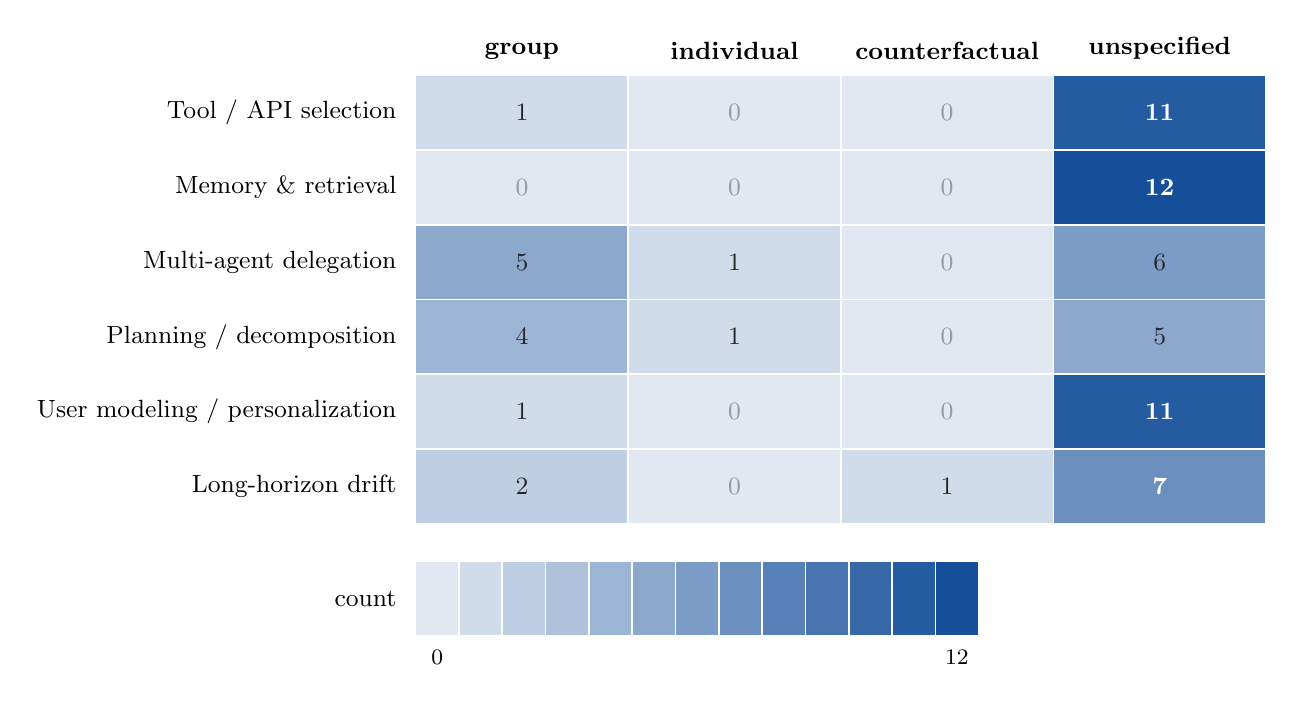
\begin{tikzpicture}[x=1cm,y=1cm]
  \def\cw{2.7}  % cell width
  \def\ch{0.95} % cell height
  % --- column headers (4 fairness dimensions) ---
  \foreach \cx/\lab in {0/group, 1/individual, 2/counterfactual, 3/unspecified}{%
    \node[font=\small\bfseries,anchor=south] at (\cx*\cw+0.5*\cw,6*\ch+0.08) {\lab};}
  % --- row labels (components), top row r=0 at top => grid y = 5-r ---
  \foreach \ry/\lab in {5/{Tool / API selection}, 4/{Memory \& retrieval},
        3/{Multi-agent delegation}, 2/{Planning / decomposition},
        1/{User modeling / personalization}, 0/{Long-horizon drift}}{%
    \node[font=\small,anchor=east] at (-0.12,\ry*\ch+0.5*\ch) {\lab};}
  % --- cells: \bcfcell{col}{gridy}{count}{maxcount}{w}{h}, max=12 ---
  % Tool/API (gridy 5)
  \bcfcell{0}{5}{1}{12}{\cw}{\ch}  \bcfcell{1}{5}{0}{12}{\cw}{\ch}  \bcfcell{2}{5}{0}{12}{\cw}{\ch}  \bcfcell{3}{5}{11}{12}{\cw}{\ch}
  % Memory & retrieval (gridy 4)
  \bcfcell{0}{4}{0}{12}{\cw}{\ch}  \bcfcell{1}{4}{0}{12}{\cw}{\ch}  \bcfcell{2}{4}{0}{12}{\cw}{\ch}  \bcfcell{3}{4}{12}{12}{\cw}{\ch}
  % Multi-agent delegation (gridy 3)
  \bcfcell{0}{3}{5}{12}{\cw}{\ch}  \bcfcell{1}{3}{1}{12}{\cw}{\ch}  \bcfcell{2}{3}{0}{12}{\cw}{\ch}  \bcfcell{3}{3}{6}{12}{\cw}{\ch}
  % Planning/decomposition (gridy 2)
  \bcfcell{0}{2}{4}{12}{\cw}{\ch}  \bcfcell{1}{2}{1}{12}{\cw}{\ch}  \bcfcell{2}{2}{0}{12}{\cw}{\ch}  \bcfcell{3}{2}{5}{12}{\cw}{\ch}
  % User modeling/personalization (gridy 1)
  \bcfcell{0}{1}{1}{12}{\cw}{\ch}  \bcfcell{1}{1}{0}{12}{\cw}{\ch}  \bcfcell{2}{1}{0}{12}{\cw}{\ch}  \bcfcell{3}{1}{11}{12}{\cw}{\ch}
  % Long-horizon drift (gridy 0)
  \bcfcell{0}{0}{2}{12}{\cw}{\ch}  \bcfcell{1}{0}{0}{12}{\cw}{\ch}  \bcfcell{2}{0}{1}{12}{\cw}{\ch}  \bcfcell{3}{0}{7}{12}{\cw}{\ch}
  % --- legend (sequential shade 0 .. 12) ---
  \begin{scope}[shift={(0,-1.5*\ch)}]
    \node[font=\small,anchor=east] at (-0.12,0.5*\ch) {count};
    \foreach \i in {0,1,...,12}{%
      \pgfmathsetmacro{\lop}{0.12+0.83*(\i/12)}%
      \fill[bcfblue,fill opacity=\lop] (\i*0.55,0) rectangle (\i*0.55+0.55,\ch);
      \draw[white,line width=0.6pt] (\i*0.55,0) rectangle (\i*0.55+0.55,\ch);}
    \node[font=\footnotesize,anchor=north] at (0.275,-0.05) {0};
    \node[font=\footnotesize,anchor=north] at (12*0.55+0.275,-0.05) {12};
  \end{scope}
\end{tikzpicture}%
}
\caption{Coverage matrix (agent component $\times$ fairness dimension), cells shaded by paper count (single-hue, colorblind-safe blue). The counterfactual column holds exactly one nonzero cell (long-horizon drift, \cite{she2025fairsense}); the unspecified column dominates with 52 of 68 component-branch entries.}
\label{fig:coverage}
\end{figure*}

\emph{Takeaway: the counterfactual column is near-empty, holding exactly one entry (she2025fairsense) across all six components, while 52 of the 68 component-branch entries fall in the unspecified column.}

This is a structural inversion of need. The counterfactual flip (re-running the same agent on a profile altered only in a protected attribute and asking whether the trajectory changed) is the natural operationalization of the agentic fairness question: "would the agent have \emph{acted} differently for another demographic?" Group-level metrics, computed over output distributions, cannot directly answer this. In BCF terms, the counterfactual swap is the procedure that produces D2's $\Delta_c$, which enters the conduction equation. The dimension BCF-based auditing most requires is precisely the dimension the field has least applied. The lone exemplar is not a genuine exception: \cite{she2025fairsense} is adjacent and non-agentic (marked [$\dagger$] in \S{}3.6, a generic ML-system drift simulator never applied to an instrumented LLM-agent trajectory), so the counterfactual column is empty of properly agentic counterfactual auditing.

The gap is one of application, not missing methods. The counterfactual tooling exists: CFR/MASD in \cite{mayilvaghanan2026counterfactual}; the CAFFE framework for systematic counterfactual evaluation \cite{parziale2025systematic}; the SCOPE stereotyped-prompt dataset \cite{parziale2026scope}; the equal-access counterfactual audit \cite{amirimargavi2026equal}; and intervention-consistency testing \cite{basu2026names}. All five sit in the evaluation-metrics-benchmarks branch; none has been wired through any of the six agent-pipeline components as a primary measurement instrument.

\emph{Takeaway (Figure~\ref{fig:coverage}): Across all six agent components, counterfactual fairness (the dimension BCF-based auditing requires for $\Delta_c$ estimation) appears in exactly one of the 68 component-branch entries; the GENERATE conduction signature remains empirically uncharted, while AMPLIFY is observed but seldom named as a fairness mechanism.}

\subsection{Group Fairness Clusters Only Where Decisions are Explicit}

Where a formal fairness dimension is invoked, it is overwhelmingly group fairness, and it clusters where the agent emits an explicit, attributable decision: \textbf{multi-agent delegation} (5 group-framed papers, 1 individual) and \textbf{planning/decomposition} (4 group, 1 individual). These are the components whose outputs most resemble the binary decisions that group-parity metrics were designed for: a role assignment, a debate verdict, a task allocation, a discrete approval or denial. Multi-agent work measures disparity across agent personas and emergent group outcomes \cite{madigan2025emergent,nguyen2025social,li2025from,mirza2025malibu}; planning work measures decision and allocation disparity \cite{li2025actions,hall2025guiding,parziale2026once}. \textbf{Formalization tracks decision explicitness, not harm severity}: components exposing a clean decision variable attract group metrics; components whose harm is diffuse (retrieval ranking, memory accumulation, user-model inference) do not, regardless of how consequential those harms may be.

\subsection{Tool, Memory, and Personalization Harms are Documented but Rarely Formalized}

Three components are dominated almost entirely by the unspecified column: \textbf{memory and retrieval} (0 formal, 12 unspecified), \textbf{tool/API selection} (1 group, 11 unspecified), and \textbf{user modeling/personalization} (1 group, 11 unspecified). Memory and retrieval is the starkest case: not a single paper names a formal fairness dimension, despite substantial evidence of real harm -- RAG degrading fairness even for vigilant users \cite{hu2024free}, multi-turn fairness erosion \cite{fan2024fairmt}, belief drift from accumulating context \cite{geng2025accumulating,simhi2026old}, and adversarial retrieval-store poisoning \cite{wang2025bias}. These papers demonstrate disparity convincingly but do not measure it against group, individual, or counterfactual criteria, instead reporting bespoke or qualitative gaps. The same pattern holds for tool selection \cite{blankenstein2025biasbusters,sneh2025tooltweak} and personalization \cite{kantharuban2024stereotype,pawar2025presumed,mire2025rejected,tonneau2026different}.

Harm outside the formal-fairness vocabulary cannot be benchmarked, tracked across model versions, or compared across systems. Documentation without formalization is the field's modal state for half the agent pipeline, and it directly drives the P5 Measurement-adequacy gap the BCF identifies.

\subsection{The Locus $\times$ BCF-Operator Grid}

Figure~\ref{fig:coverage} cross-tabulates component with fairness \emph{dimension}; Figure~\ref{fig:operator} cross-tabulates component-as-locus with BCF conduction \emph{operator} (ATTENUATE / PRESERVE / AMPLIFY / GENERATE). The two are complementary: Figure~\ref{fig:coverage} reveals what formal vocabulary is used; Figure~\ref{fig:operator} reveals what \emph{transformation} of disparity is being empirically studied versus merely assumed.

\textbf{Construction.} Each corpus paper with a component tag is assigned a conduction operator based on whether it documents disparity attenuation (a debiasing intervention reducing $\Delta_c$ at that component), preservation (disparity passes through unchanged), amplification (disparity increases), or generation (disparity arises at that component from nominally zero input, the agentic phenomenon with no single-model analogue). A paper can carry multiple operator tags.

\begin{figure*}[htbp]
\centering
\resizebox{\textwidth}{!}{%
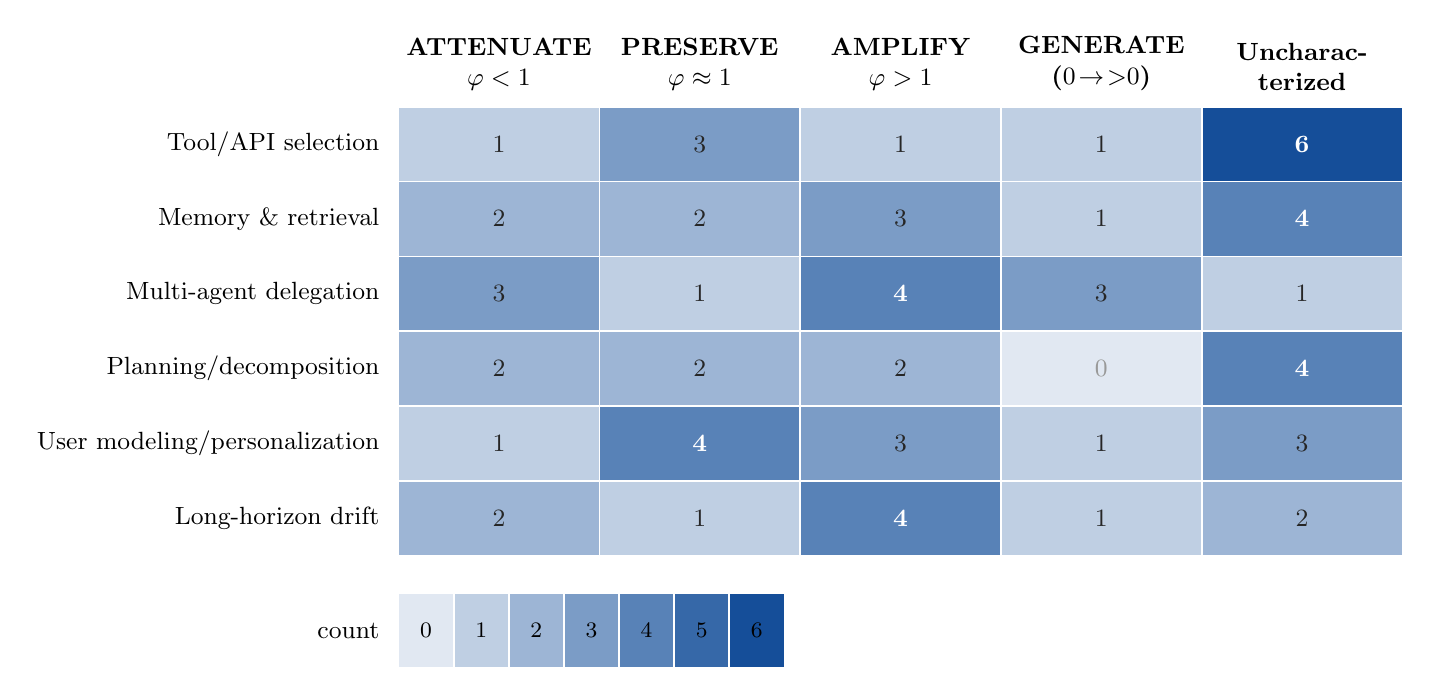
\begin{tikzpicture}[x=1cm,y=1cm]
  \def\cw{2.55} % cell width
  \def\ch{0.95} % cell height
  % --- column headers (5 conduction operators) ---
  \node[font=\small\bfseries,anchor=south,align=center] at (0*\cw+0.5*\cw,6*\ch+0.08) {ATTENUATE\\$\varphi<1$};
  \node[font=\small\bfseries,anchor=south,align=center] at (1*\cw+0.5*\cw,6*\ch+0.08) {PRESERVE\\$\varphi\approx1$};
  \node[font=\small\bfseries,anchor=south,align=center] at (2*\cw+0.5*\cw,6*\ch+0.08) {AMPLIFY\\$\varphi>1$};
  \node[font=\small\bfseries,anchor=south,align=center] at (3*\cw+0.5*\cw,6*\ch+0.08) {GENERATE\\($0\!\rightarrow\!{>}0$)};
  \node[font=\small\bfseries,anchor=south,align=center] at (4*\cw+0.5*\cw,6*\ch+0.08) {Uncharac-\\terized};
  % --- row labels (loci) ---
  \foreach \ry/\lab in {5/{Tool/API selection}, 4/{Memory \& retrieval},
        3/{Multi-agent delegation}, 2/{Planning/decomposition},
        1/{User modeling/personalization}, 0/{Long-horizon drift}}{%
    \node[font=\small,anchor=east] at (-0.12,\ry*\ch+0.5*\ch) {\lab};}
  % --- cells: \bcfcell{col}{gridy}{count}{max}{w}{h}, max=6 ---
  % Tool/API (gridy 5): 1 3 1 1 6
  \bcfcell{0}{5}{1}{6}{\cw}{\ch} \bcfcell{1}{5}{3}{6}{\cw}{\ch} \bcfcell{2}{5}{1}{6}{\cw}{\ch} \bcfcell{3}{5}{1}{6}{\cw}{\ch} \bcfcell{4}{5}{6}{6}{\cw}{\ch}
  % Memory & retrieval (gridy 4): 2 2 3 1 4
  \bcfcell{0}{4}{2}{6}{\cw}{\ch} \bcfcell{1}{4}{2}{6}{\cw}{\ch} \bcfcell{2}{4}{3}{6}{\cw}{\ch} \bcfcell{3}{4}{1}{6}{\cw}{\ch} \bcfcell{4}{4}{4}{6}{\cw}{\ch}
  % Multi-agent delegation (gridy 3): 3 1 4 3 1
  \bcfcell{0}{3}{3}{6}{\cw}{\ch} \bcfcell{1}{3}{1}{6}{\cw}{\ch} \bcfcell{2}{3}{4}{6}{\cw}{\ch} \bcfcell{3}{3}{3}{6}{\cw}{\ch} \bcfcell{4}{3}{1}{6}{\cw}{\ch}
  % Planning/decomposition (gridy 2): 2 2 2 0 4
  \bcfcell{0}{2}{2}{6}{\cw}{\ch} \bcfcell{1}{2}{2}{6}{\cw}{\ch} \bcfcell{2}{2}{2}{6}{\cw}{\ch} \bcfcell{3}{2}{0}{6}{\cw}{\ch} \bcfcell{4}{2}{4}{6}{\cw}{\ch}
  % User modeling/personalization (gridy 1): 1 4 3 1 3
  \bcfcell{0}{1}{1}{6}{\cw}{\ch} \bcfcell{1}{1}{4}{6}{\cw}{\ch} \bcfcell{2}{1}{3}{6}{\cw}{\ch} \bcfcell{3}{1}{1}{6}{\cw}{\ch} \bcfcell{4}{1}{3}{6}{\cw}{\ch}
  % Long-horizon drift (gridy 0): 2 1 4 1 2
  \bcfcell{0}{0}{2}{6}{\cw}{\ch} \bcfcell{1}{0}{1}{6}{\cw}{\ch} \bcfcell{2}{0}{4}{6}{\cw}{\ch} \bcfcell{3}{0}{1}{6}{\cw}{\ch} \bcfcell{4}{0}{2}{6}{\cw}{\ch}
  % --- legend (sequential shade 0 .. 6) ---
  \begin{scope}[shift={(0,-1.5*\ch)}]
    \node[font=\small,anchor=east] at (-0.12,0.5*\ch) {count};
    \foreach \i in {0,1,...,6}{%
      \pgfmathsetmacro{\lop}{0.12+0.83*(\i/6)}%
      \fill[bcfblue,fill opacity=\lop] (\i*0.7,0) rectangle (\i*0.7+0.7,\ch);
      \draw[white,line width=0.6pt] (\i*0.7,0) rectangle (\i*0.7+0.7,\ch);
      \node[font=\footnotesize] at (\i*0.7+0.35,0.5*\ch) {\i};}
  \end{scope}
\end{tikzpicture}%
}
\caption{Locus $\times$ BCF conduction-operator grid, cells shaded by paper count (single-hue, colorblind-safe blue; row sums total 68). The GENERATE column is the genuinely empty quadrant (column sum 7): planning/decomposition has no GENERATE entry and tool selection registers a single GENERATE paper, marking the highest-priority measurement gaps. AMPLIFY, by contrast, is mid-populated (column sum 17, comparable to PRESERVE and ATTENUATE), so its cells are studied but rarely formalized rather than uninstrumented.}
\label{fig:operator}
\end{figure*}

\emph{Takeaway (Figure~\ref{fig:operator}): GENERATE (column sum 7) is the genuinely under-instrumented operator: planning/decomposition has no GENERATE entry and tool selection registers only one, the highest-priority measurement gaps for BCF-guided empirical work. AMPLIFY (column sum 17) is mid-populated, comparable to PRESERVE and ATTENUATE, so the agentic amplification of disparity is empirically attested but seldom named in formal fairness terms.}

The most consequential observation is that the \textbf{GENERATE} operator (disparity arising at a pipeline edge from nominally unbiased inputs, the formal signature of the agentic multiplier in P3) appears in only a handful of papers. For multi-agent delegation, \cite{nguyen2025social} and \cite{madigan2025emergent} provide the clearest evidence of generation (bias emerging in interaction among individually measured-to-be-unbiased agents); for tool selection, \cite{blankenstein2025biasbusters} documents the selection-skew signature from tool-description surface features alone. Outside these, the GENERATE column is largely empty. The audit of \S{}6 is designed to probe this empirical frontier.

\subsection{Synthesis and Differentiation}

Four regularities emerge from the combined Figure~\ref{fig:coverage}/Figure~\ref{fig:operator} analysis.

First, \textbf{formalization tracks decision explicitness, not harm severity}: components that emit a clean decision variable attract formal metrics; diffuse-harm components do not.

Second, \textbf{the formal vocabulary thins toward the counterfactual and toward GENERATE/AMPLIFY} exactly as the evaluation question shifts from "what did the agent output?" toward the distinctively agentic questions: "would it have acted differently?" and "did the pipeline produce disparity it did not inherit?"

Third, \textbf{the modal corpus paper documents disparity without naming a fairness dimension or a conduction operator}: 52 of the 68 component-branch entries sit in the unspecified column of Figure~\ref{fig:coverage}, and most locus $\times$ operator cells in Figure~\ref{fig:operator} are under-populated. The field is evidence-rich and formalization-poor.

Fourth, the BCF coordinate system makes the gaps precise and actionable: the empty cells of Figure~\ref{fig:operator} are specific (component, operator) pairs that targeted experiments can populate using the counterfactual-perturbation machinery already available \cite{parziale2025systematic,mayilvaghanan2026counterfactual,basu2026names}.

This analysis also sharpens the differentiation from neighboring work (Table~\ref{tab:survey-comparison} in \S{}1.4). Where \cite{chu2024fairness} organizes single-turn LLM fairness by metric and \cite{gallegos2024bias} by datasets and mitigation, neither resolves \emph{where in an acting pipeline} a disparity originates. Where \cite{mohammadi2025evaluation} treats fairness as one sub-topic of agent evaluation and \cite{vatsal2026agentic} as a subdimension of a seven-dimensional clinical taxonomy, neither makes component coverage its unit of analysis. Where \cite{ranjan2025fairness} proposes a framework for fairness in multi-agent AI broadly, it does not operate at the LLM-agent component level or develop the conduction-operator analysis. By projecting the corpus onto the component $\times$ operator grid, this survey converts the measurement gap from an assertion into a structured coordinate (the empty counterfactual column and the under-populated GENERATE/AMPLIFY cells) and hands \S{}8 a concrete, BCF-keyed research target.

\section{Open Problems and Research Agenda}

The coverage analysis of \S{}7 converts the measurement gap into precise coordinates: (component, operator) cells in Figure~\ref{fig:operator} that remain empirically uncharacterized, P5 Measurement-adequacy cells no existing benchmark populates, and BCF propositions with weak empirical grounding. A governance thread runs through all six problems below. Agents operate in hiring, lending, healthcare, and public-benefits adjudication, where disparate treatment across race, gender, socioeconomic status, dialect, and their intersections carries direct legal weight. The EU AI Act (Regulation 2024/1689) classifies high-risk AI systems in employment, credit, and essential-service sectors as subject to bias-testing and transparency requirements \cite{parliament2024regulation}; the NIST AI Risk Management Framework specifies bias evaluation as a component of AI governance \cite{nist2023artificial}; New York City Local Law 144 requires automated employment decision tools to undergo annual bias audits; and EEOC guidance applies Title VII disparate-impact standards to algorithmic hiring tools. None of these frameworks specifies what a fairness audit of an \emph{acting agent} must cover, and the measurement infrastructure of \S{}4.4 cannot discharge those requirements. Each missing metric, dataset, or system design is also a missing regulatory instrument.

\subsection{Unpopulated P5 cells: benchmarks for acting agents}

P5 Measurement-adequacy requires that a metric detect non-zero $\Delta_c$ at a given component independently of all others. The benchmark inventory in \S{}4.4 shows no existing benchmark satisfies P5 for any of the six agent-pipeline components at the action level.

Dominant fairness benchmarks score answers, not actions. Clinical fairness sets define the ceiling of current practice: FairMedQA evaluates demographic bias in medical QA \cite{xiao2025fairmedqa}; mFARM assembles multi-faceted harm assessment for clinical decision support \cite{adappanavar2025mfarm}; MedEqualQA probes consistency through counterfactual demographic edits \cite{ghosh2025medequalqa}; and the health equity toolbox surfaces harms at the level of generated text \cite{pfohl2024toolbox}. Each stops at the QA boundary. None measures what a clinical acting agent does when selecting which guideline tool to invoke, which prior note to retrieve, whether to escalate, or how it sequences a multi-step workup. Studies scoring actions confirm the divergence: agent decisions reveal biases absent from token-level probes \cite{li2025actions}, and decomposing unfairness in a tool-using chest X-ray agent attributes $\Delta_c$ to specific pipeline stages invisible to answer-level scoring \cite{xu2026ducx}. Existing evaluation frameworks (AgentBench \cite{liu2024agentbench}, WebArena \cite{zhou2024webarena}, SWE-bench \cite{jimenez2024swe}, OSWorld \cite{xie2024osworld}, and $\tau$-bench \cite{yao2024taubench}) are not demographically instrumented. OSWorld and $\tau$-bench score trajectory-level action and tool-use policy compliance respectively, yet both evaluate capability rather than fairness across demographic counterfactuals and cannot be repurposed without the paired-world $\sigma$ instrumentation specified below.

A system can be near-parity on FairMedQA and still route, escalate, or order differently across demographic counterfactuals once it acts, because $\Delta_c$ enters through tool routing and retrieval rather than the final string. Certifying agents with QA benchmarks licenses deployment on evidence that does not bind the deployed behavior, precisely the accountability gap EU AI Act Article 10 and NIST AI RMF Measure 2.5 are meant to close.

\begin{sloppypar}\textbf{Concrete first step.} A minimal acting-agent fairness benchmark requires: (i) consequential-task environments (e.g., clinical triage, hiring screening, loan underwriting) in which an agent can take multiple discrete actions; (ii) counterfactual profile pairs differing only in a demographic signal, following the CAFFE/SCOPE design \cite{parziale2025systematic,parziale2026scope}; (iii) logging of all intermediate actions (tool invocations, retrieval queries, routing decisions) per counterfactual pair; and (iv) reporting of per-edge $\Delta_c$ alongside the final-verdict CFR/MASD. FairMedAgent, described in \S{}6.4, is one instantiation for the clinical domain; comparable instruments are needed for hiring and lending, where legal audit requirements are already in force.\end{sloppypar}

\subsection{Unmeasured $\varphi_{\mathrm{fb}}$ recurrence: long-horizon and compounding fairness}

The feedback-recurrence term $\Delta^{(t+1)}$ = $\varphi_{\mathrm{fb}}$ $\cdot$ $\Delta^{(t)}$ + $\Delta_{\mathrm{entry}}$ formalizes how per-step disparity compounds when an agent conditions on its own prior outputs. P3 Super-additivity applied longitudinally predicts that $\varphi_{\mathrm{fb}}$ > 1 produces exponential divergence of group outcomes across deployment cycles. No existing evaluation captures this.

Fairness is evaluated as a one-shot property, but agents persist. Implicit bias in long-term memory accumulates and propagates, reinforcing small initial skews across interactions \cite{ma2026implicit}. Sequential decision-making theory establishes the formal stakes: static per-step fairness constraints fail to deliver equitable long-term outcomes, and equal long-term benefit requires reasoning about how present decisions reshape future eligibility \cite{hu2022achieving,xu2024adapting}. Training on a model's own synthetic outputs amplifies bias across generations \cite{wyllie2024fairness}, and self-consuming performative loops compound the effect at deployment \cite{wang2026observations}. No study has evaluated an LLM agent against a formal long-term fairness criterion over a realistic multi-session deployment, so the theory and the LLM-drift empirics \cite{fan2024fairmt,ma2026implicit,liu2025truth} remain unjoined.

\textbf{Concrete first step.} Define a \textbf{longitudinal disparity index} (LDI) as the ratio of group-outcome divergence at turn $T$ to turn 1, estimated by simulation over a synthetic trajectory of $T$ interactions using the recurrence $\Delta^{(t+1)}$ = $\varphi_{\mathrm{fb}}$ $\cdot$ $\Delta^{(t)}$ + $\Delta_{\mathrm{entry}}$. Parameterize $\varphi_{\mathrm{fb}}$ empirically from an existing deployed agent using the FairSense simulation tooling \cite{she2025fairsense}. A single-domain pilot (e.g., the loan-triage replication arm of \S{}6) with $T$ = 20 turns and five demographic group pairs would constitute a first binding measurement.

\subsection{Unbounded GENERATE: multi-agent fairness dynamics}

The GENERATE operator ($\varphi$ applied to nominally zero-$\Delta_c$ input) is the signature failure mode of multi-agent systems: disparity arises in the interaction among agents that are individually measured as unbiased. Figure~\ref{fig:operator} shows GENERATE is thinly populated across every locus; multi-agent delegation is the only locus with more than one GENERATE entry, despite the strongest theoretical and empirical motivation.

Bias can \emph{emerge} from interaction even among agents whose individual outputs are measured as near-parity. \cite{madigan2025emergent} formalizes emergent bias in multi-agent decision systems as a property of the collective rather than any constituent; \cite{nguyen2025social} documents bias emerging, propagating, and amplifying through agent-to-agent communication. Disparity in these settings depends on communication topology, role-assignment structure, and message-passing dynamics, none of which a per-agent audit can observe. The MALIBU benchmark \cite{mirza2025malibu} surfaces implicit bias in multi-agent assignments but does not measure the GENERATE operator specifically.

\textbf{Concrete first step.} Design a \textbf{GENERATE-detection probe}: a multi-agent task in which each constituent agent is individually certified as CFR = 0 on a single-turn benchmark, then assembled into a two-agent delegation. Measure the CFR of the delegation. Any non-zero CFR at the delegation level is GENERATE evidence; the difference between delegation-level and max(constituent) CFR estimates the GENERATE amplitude for that topology. The probe requires only the counterfactual evaluation machinery of \cite{mayilvaghanan2026counterfactual} and any existing two-agent framework \cite{wu2023autogen}.

\subsection{Intersectional and sociotechnical harms in deployment}

BCF D2 defines $\Delta_c$ as a counterfactual disparity over a single protected attribute; real deployment harms are intersectional (jointly over multiple attributes) and sociotechnical (conditioned on deployment context and model parameters together). The current formalization is a first-order approximation.

Bias research frequently isolates one protected attribute on a clean benchmark, but real deployments harm people at intersections. \cite{crenshaw1989demarginalizing} showed that treating race and sex as separable axes erases the distinct harm borne at their intersection, and \cite{foulds2020intersectional} supplies the corresponding formal criterion (differential fairness over joint subgroups), which the $\Delta_c^{A \times B}$ extension below estimates. The largest-scale evidence is unambiguous: sociodemographic biases in LLM medical decision-making produce differential management recommendations at clinical scale, with race, gender, and socioeconomic status interacting \cite{omar2025sociodemographic}; a mortgage underwriting experiment documents racial disparities in lending \cite{bowen2024measuring}; and judicial fairness evaluation finds systematic differential treatment across defendant demographics \cite{hu2025llms}. Intersectional treatment is specifically flagged in algorithmic hiring regulation \cite{raghavan2020mitigating}.

\textbf{Concrete first step.} Extend D2 to an intersectional counterfactual disparity $\Delta_c^{A \times B}$ defined as the $\Delta_c$ estimated under joint swap of attributes A and B minus the sum of the marginal $\Delta_c$ values, capturing the interaction term; a non-zero interaction term operationalizes the differential-fairness violation \cite{foulds2020intersectional} that single-attribute auditing cannot see. Apply this to the \S{}6 audit's hiring task with a 2$\times$2 race-by-gender counterfactual design; this requires only doubling the profile set and is immediately feasible.

\subsection{Empty operator rows of the conduction grid: governance and standardized auditing}

The ATTENUATE rows of Figure~\ref{fig:operator} are partially populated, but the formal connection between a mitigation's claimed ATTENUATE effect and its BCF-level $\varphi$ value is never established: no paper reports how much $\varphi_e$ decreases at a specific pipeline edge following a given intervention. This is a P4 Mitigation-matching gap.

There is no shared standard for what constitutes a fairness audit of an LLM agent. The ingredients exist: the CAFFE counterfactual framework \cite{parziale2025systematic}, the SCOPE dataset \cite{parziale2026scope}, the LangFair evaluation toolkit \cite{bouchard2024bring}, the intervention-consistency test \cite{basu2026names}, and the dataset survey \cite{zhang2025datasets}. No governance instrument standardizes them into a repeatable, comparable audit of an \emph{acting} system. The regulatory field has outpaced the measurement infrastructure: the EU AI Act \cite{parliament2024regulation}, the NIST AI RMF \cite{nist2023artificial}, NYC Local Law 144, and EEOC disparate-impact analysis each impose bias-testing requirements, yet none specifies what those audits must cover for an acting agent rather than a static classifier.

\textbf{Concrete first step.} Draft a \textbf{minimum audit specification} for acting agents with four components: (i) a protocol for constructing counterfactual profile sets (building on \cite{parziale2025systematic}); (ii) a required metric set covering, at minimum, per-component CFR, tool-invocation disparity, and escalation-rate disparity, aligned with the BCF's D2 definition; (iii) a standardized reporting template with per-component $\Delta_c$ values and the conduction-operator classification (ATTENUATE/PRESERVE/AMPLIFY/GENERATE) for each active edge; and (iv) a recourse specification covering what information must be logged to enable post-hoc attribution and contestation. Per-component $\Delta_c$ attribution is a natural substrate for algorithmic recourse \cite{karimi2022recourse}: localizing a disparity to a specific pipeline edge tells an affected person what to contest and tells the operator which edge to change, which a single endpoint-level parity number cannot. This specification can be submitted as a technical standard proposal to the NIST AI 100-1 framework revision process.

\subsection{Mitigation at the agent level, not the token level}

P4 Mitigation-matching states that an intervention is matched if it operates at the same pipeline locus as the disparity it corrects. The mitigation map in \S{}5 shows the ATTENUATE column of Figure~\ref{fig:operator} is populated almost entirely by token-level interventions, which are mismatched to the six agent-pipeline loci where AMPLIFY and GENERATE operators are documented.

The mitigation literature overwhelmingly intervenes on model outputs: debiasing prompts \cite{furniturewala2024thinking,li2024prompting}, preference optimization \cite{allam2024biasdpo,bai2022constitutional}, inference-time activation steering \cite{li2025fairsteer}, and output guardrails \cite{dong2024building}. These operate on tokens. But \S{}3 locates agentic harm in actions and architecture: which tool is chosen, what is retrieved into context, how roles are assigned, how a plan is decomposed. Token-level debiasing leaves these channels untouched. The few process-aware interventions point the way: balanced-retrieval agents \cite{singh2025biasb}, bias-aware retrieval \cite{singh2025bias}, identity anonymization to neutralize role-induced debate bias \cite{choi2025identity}, and multi-agent debiasing frameworks \cite{owens2024multi,xu2024mitigating}. No unified framework simultaneously addresses tool-selection, memory-accumulation, and delegation loci.

\textbf{Concrete first step.} Implement a \textbf{component-keyed guardrail layer} as a proof of concept: a wrapper that intercepts the agent's action proposal at each of the three highest-priority AMPLIFY/GENERATE loci identified in Figure~\ref{fig:operator} (tool selection, multi-agent delegation, long-horizon accumulation) and applies a targeted $\Delta_c$ reduction intervention before action execution. The three interventions are, respectively: a demographic-blind re-ranking of tool candidates, a role-assignment audit against an assignment-disparity threshold, and a memory-hygiene filter. Evaluate the wrapper using the \S{}6 audit's C1 to C3 configurations, reporting per-edge $\varphi_e$ before and after to directly test P4 Mitigation-matching.

\subsection{Synthesis}

The autonomy that makes agents valuable (acting, persisting, delegating, self-conditioning) is exactly what QA-level measurement, single-shot certification, and token-level mitigation cannot observe. Closing the gap requires instruments, protocols, and interventions defined over trajectories and actions, governed at the system level, and reported in a format auditors and regulators can use. The BCF supplies the coordinate system; the six open problems above specify the cells to fill.


\section{Conclusion}

LLM-based agents select tools, accumulate memories across turns, delegate subtasks across role-assigned subagents, decompose goals into multi-step plans, adapt to inferred user identities, and persist behavior over long horizons \cite{wang2024survey,xi2023rise}. Each pipeline stage is a distinct locus at which demographic disparity can enter, propagate, and compound into consequential harm. The Bias Conduction Framework introduced in \S{}3.0 formalizes this structure: D1 defines the agent loop $\langle$$\pi$, T, M, R$\rangle$; D2 defines component counterfactual disparity $\Delta_c$ via trace-replay; D3 defines the conduction operators (ATTENUATE $\varphi < 1$, PRESERVE $\varphi \approx 1$, AMPLIFY $\varphi > 1$, GENERATE $\varphi$ on zero input); the conduction equation $\Delta_\tau$ $\approx$ $\Sigma_c$ $\Delta_c$ $\cdot$ $\Pi$ $\varphi_e$ with feedback recurrence $\Delta^{(t+1)}$ = $\varphi_{\mathrm{fb}}$ $\cdot$ $\Delta^{(t)}$ + $\Delta_{\mathrm{entry}}$ derives trajectory disparity from per-component contributions; and five propositions (P1 Locality, P2 Masking, P3 Super-additivity, P4 Mitigation-matching, P5 Measurement-adequacy) characterize when component-level auditing is necessary, sufficient, and policy-relevant.

This survey presents the first dedicated taxonomy of fairness in LLM-based agents organized by component: tool and API selection (\S{}3.1), memory and retrieval (\S{}3.2), multi-agent delegation and role assignment (\S{}3.3), planning and decomposition (\S{}3.4), user modeling and personalization (\S{}3.5), and long-horizon trajectory drift (\S{}3.6), with a cross-cutting account of how component-level harms compound into the agentic multiplier (\S{}3.7, P3). The evaluation survey (\S{}4) characterizes group, individual, and counterfactual metric families lifted to agent trajectories, generalizes the CFR and MASD statistics of \cite{mayilvaghanan2026counterfactual} across all pipeline components, and documents in Table~\ref{tab:benchmarks} that nearly every existing benchmark (clinical fairness sets \cite{xiao2025fairmedqa,adappanavar2025mfarm,ghosh2025medequalqa}, hiring and lending audits \cite{an2025measuring,azime2025accept}, compositional evaluation suites \cite{wang2024ceb}) scores model outputs rather than agent actions. The mitigation survey (\S{}5) applies the P4 Mitigation-matching principle across prompt-level interventions \cite{furniturewala2024thinking,li2024prompting}, alignment-stage approaches \cite{allam2024biasdpo,bai2022constitutional}, architectural guardrails \cite{dong2024building}, and the emerging class of process-level and multi-agent debiasing strategies \cite{owens2024multi,choi2025identity,ki2025multiple}. The coverage analysis (\S{}7) quantifies the gap: 52 of 68 component-branch entries sit in the unspecified column of Figure~\ref{fig:coverage}; the counterfactual column (required to compute D2's $\Delta_c$) contains exactly one entry across all six components; and the GENERATE/AMPLIFY cells of Figure~\ref{fig:operator} are the least populated despite being the loci of distinctively agentic harm. The controlled cross-framework audit (\S{}6) supports P2 (Masking), where score-level disparity (MASD of roughly 8 to 11 points) is several times the binary advance-rate disparity (0.08 to 0.17) in every configuration, but finds no monotone amplification with scaffolding complexity (H2 is not borne out at this scale), with a scaled benchmark remaining future work.

LLMs and LLM-based agents are deployed in hiring \cite{veldanda2023emily,wilson2024gender,nghiem2024you}, clinical decision support \cite{poulain2024bias,omar2025sociodemographic}, lending \cite{bowen2024measuring,feng2023empowering}, and education \cite{weissburg2024llms} (much of the cited evidence is audit or evaluation in these settings rather than confirmed operational deployment), subject to regulatory requirements (EU AI Act \cite{parliament2024regulation}, NIST AI RMF \cite{nist2023artificial}, NYC Local Law 144, EEOC disparate-impact guidance) that no current acting-agent fairness benchmark is equipped to satisfy. Feedback recurrence documented by \cite{wyllie2024fairness} and \cite{wang2026observations}, memory accumulation characterized by \cite{ma2026implicit}, and the sequential fairness theory of \cite{hu2022achieving,xu2024adapting} collectively predict that systems fair at any single step can drive divergent cumulative outcomes across groups over deployment cycles. The measurement gap documented here is therefore also a gap in accountability infrastructure. The immediate priority is benchmark construction for acting agents: evaluation infrastructure that scores trajectories and decisions rather than tokens and outputs, applies counterfactual demographic perturbations at the action level \cite{parziale2025systematic,amirimargavi2026equal,basu2026names}, and covers the per-component, per-edge $\Delta_c$ granularity the BCF specifies. That infrastructure is the precondition for every subsequent advance in mitigation (P4), governance (\S{}8.5), and longitudinal auditing (\S{}8.2). The conceptual vocabulary and the first components of the counterfactual tooling exist. The gap is instrumentation.


\subsection{Ethical considerations, societal impact, and limitations of this survey}

The taxonomy and evaluation framework this work advances can be used both to \emph{audit and constrain} unfair agent behavior and to \emph{reverse-engineer and evade} such constraints. We address this dual-use concern and the additional limitations that bear on how the survey's findings should be interpreted.

\subsubsection{Dual-use of the taxonomy and BCF framework}

The BCF's conduction-operator vocabulary identifies which pipeline edges are AMPLIFY or GENERATE loci and which mitigation interventions reduce $\varphi_e$ at each edge. The same information can be used adversarially: knowing that tool-description metadata is a GENERATE locus \cite{sneh2025tooltweak} could guide an actor who wishes to steer an agent's routing by manipulating tool descriptions, and the fact that memory-accumulation is an AMPLIFY locus could inform retrieval-store poisoning attacks \cite{wang2025bias} calibrated to exploit that amplification. The survey discloses these mechanisms because responsible auditing requires understanding them. Practitioners who use the BCF as an audit template should also treat it as an adversarial-risk checklist, evaluating deployed agents for susceptibility to targeted disparity injection at the loci this taxonomy identifies.

\subsubsection{Academic-vs-legal fairness gap}

The fairness criteria formalized in \S{}2.1 and operationalized throughout the survey (demographic parity, equalized odds, counterfactual fairness) are academic constructs whose relationship to the legal standards governing high-stakes AI deployment is partial and contested. Disparate-impact doctrine under Title VII (hiring), the Equal Credit Opportunity Act (lending), and the EU AI Act's non-discrimination provisions each impose distinct evidentiary standards, burden-of-proof structures, and remediation requirements that academic fairness metrics do not automatically satisfy. Specifically: (i) a system achieving statistical demographic parity may still constitute unlawful disparate treatment under intent-based theories; (ii) a system failing the counterfactual flip test may satisfy legal requirements if the disparity is justified by legitimate business necessity; and (iii) the granular per-component $\Delta_c$ measurements the BCF requires are not currently mandated by any regulatory framework, meaning deployers may satisfy legal compliance while exhibiting large action-level disparities invisible to regulators. We encourage legal scholars and regulators to engage with the BCF's measurement proposals as inputs to standard-setting processes now underway under the EU AI Act and NIST AI RMF frameworks.

\subsubsection{English- and US/EU-centric corpus positionality}

The 202-paper corpus was assembled from English-language academic venues (arXiv, ACL Anthology, ACM DL, NeurIPS\allowbreak/\allowbreak ICML\allowbreak/\allowbreak ICLR, FAccT, Nature), all of which have geographic and linguistic concentrations in the United States and Western Europe. Several structural biases follow:

\begin{itemize}
\item \textbf{Language bias}: nearly all benchmark datasets and evaluation prompts are in English; dialect bias findings (e.g., \cite{mire2025rejected} on African American Language; \cite{lin2024assessing} on non-standard dialects) are primarily US-context findings. Bias patterns in Arabic, Hindi, Swahili, and other high-speaker-count languages are substantially underrepresented.
\item \textbf{Protected-attribute scope}: the protected attributes most frequently studied (race (primarily Black/white US framing), binary gender, and US-relevant socioeconomic status) do not map cleanly onto the protected categories, group identities, and fairness norms of other legal and cultural contexts. India's caste system, Brazil's color classification, the EU's national-origin protections, and indigenous identity frameworks are effectively absent from the corpus.
\item \textbf{High-stakes-domain coverage}: the corpus's consequential-domain evidence clusters in US hiring (name-based resume audits), US lending (mortgage underwriting), and US clinical settings (medical QA). Non-US regulatory contexts, public-benefit adjudication systems, and welfare-state service delivery are not covered.
\end{itemize}

These constraints mean the survey's findings are most directly applicable to LLM-based agents deployed in English-language, US- or EU-regulated, employment/credit/healthcare contexts; extrapolation to other contexts warrants caution. Geographic and multilingual expansion of the corpus is the highest-priority scope extension for a follow-up survey.

\subsubsection{Limitations of the audit}

The cross-framework audit of \S{}6 is controlled but modest in scale (\S{}6.5): N = 12 synthetic profiles (6 strong, 6 borderline), a decoupled 2x2 race-by-gender name counterfactual, 144 decisions, and bootstrap 95\% confidence intervals over 3000 profile resamples. The borderline tier addresses the decision-level ceiling effect that bound the earlier strong-only pilot to CFR = 0.

\begin{itemize}
\item P2 (Masking) is supported: the score-level disparity (MASD of roughly 8 to 11 points) is several times the binary advance-rate disparity (0.08 to 0.17) in every configuration. P3 / H2 (amplification with scaffold complexity) is not supported at this scale: MASD is non-monotone across C0, C2, and C3 with overlapping confidence intervals, and the audit does not reproduce the earlier small pilot's apparent monotone MASD trend. Readers should treat P2 as supported by this controlled run together with the multi-paper evidence cited throughout \S{}\S{}3--4, and P3's cross-component amplification form as a well-motivated conjecture this audit does not confirm.
\item The audit remains modest in scale (one model, Haiku 4.5; one task; one name set per cell; names that encode race and gender jointly within each label), and is a controlled measurement rather than a definitive audit. The stance is non-confirmatory by design.
\item The conduction-operator tagging in Figure~\ref{fig:operator} reflects the survey authors' interpretation of whether each cited paper's finding instantiates ATTENUATE, PRESERVE, AMPLIFY, or GENERATE at the relevant locus, not a standardized classification applied by the original authors. Some cells may be reclassified as the audit methodology matures.
\item The audit instantiates only the answer-level metrics (CFR, MASD) and the decision-action disparity. The remaining action-level metrics (tool-invocation disparity, escalation disparity, plan-allocation disparity) are specified in \S{}6.2 but require a tool-using deployment and have not been computed; their distributional properties, sensitivity, and test-retest reliability are unknown until the scaled study.
\end{itemize}

The survey's contribution is the framework, the protocol, and a controlled first measurement. The harness and data are released as a replication target; the scaled benchmark is the immediate next step (\S{}8.1).

\subsubsection{Fast-moving field and recency constraints}

The corpus cutoff is mid-2026. The LLM-agent field's publication rate has accelerated sharply since 2023 \cite{wang2024survey}, and the fairness subfield is following the same trajectory. Several developments already visible at the corpus boundary may alter the picture drawn here:

\begin{itemize}
\item \textbf{Frontier model capability shifts}: improvements in instruction-following fidelity and tool-calling reliability may change the empirical profile of which pipeline edges are AMPLIFY versus PRESERVE loci, as models become more or less sensitive to demographic cues at each stage.
\item \textbf{Regulatory enactments}: the EU AI Act's implementing acts specifying audit requirements for high-risk AI systems are expected to issue in 2025 to 2026; these may operationalize bias-testing requirements in ways that alter the alignment between academic fairness metrics and legal compliance requirements.
\item \textbf{Benchmark releases}: AgentBench \cite{liu2024agentbench}, WebArena \cite{zhou2024webarena}, and $\tau$-bench are actively adding evaluation dimensions; demographically instrumented agentic fairness evaluation may be released within these frameworks within the survey's publication window, which would partially populate the empty cells of Figure~\ref{fig:coverage}.
\end{itemize}

The coverage matrix is a snapshot of the field as of mid-2026. The BCF framework and the open-problem agenda of \S{}8 are designed to remain relevant as the empirical field changes; the specific cell counts in Figure~\ref{fig:coverage} and Figure~\ref{fig:operator} should be updated as new work appears.

\bibliographystyle{ACM-Reference-Format}
\bibliography{references}



\end{document}